\documentclass[12pt,a4paper,oneside]{report}
\usepackage{graphicx}
%\usepackage{german,a4}
\usepackage{lmodern}
\usepackage{fancyhdr}
\usepackage[utf8]{inputenc}
%\usepackage{setspace}
\usepackage[T1]{fontenc}
\usepackage{hyperref}
\usepackage[sf]{titlesec}
\usepackage{textcomp}
\usepackage{makeidx}
\usepackage{amsmath}
\usepackage[english, american]{babel}
\usepackage{listings}
\usepackage{color}
\usepackage{colortbl}
\definecolor{lightgray}{rgb}{0.8,0.8,0.8}
\definecolor{darkgreen}{rgb}{0,0.6,0}
\usepackage{pdfpages}
\usepackage{graphicx}
\usepackage{cite}
\usepackage{listings}
\usepackage{array}
\usepackage{caption}
\usepackage{subcaption}
\usepackage[font=small,labelfont=bf]{caption}
\usepackage[utf8]{inputenc}
\usepackage[compat=1.0.0]{tikz-feynman}
\usepackage{mathtools}
\usepackage{ mathrsfs }
% =====================================================
% Seite einrichten
% =====================================================
\setlength{\textwidth}{160mm} \setlength{\textheight}{235mm}
\setlength{\evensidemargin}{5mm} \setlength{\oddsidemargin}{5mm}
\setlength{\topmargin}{0mm} \setlength{\voffset}{-15mm}
\setlength{\headsep}{12mm} \setlength{\footskip}{15mm}
\setlength{\headheight}{15.1pt}

% =====================================================
% sonstige Einstellungen
% =====================================================
%\flushbottom % Textfluss schoen unten ausrichten
\footnotesep12pt % Abstand Text / Fussnote
%\setlength{\parindent}{0pt} \setlength{\abovecaptionskip}{-6pt}
%\setlength{\belowcaptionskip}{0pt} \setlength{\intextsep}{18pt}
%\renewcommand{\baselinestretch}{1.2} % Zeilenabstand
\setcounter{secnumdepth}{4}
\newcommand{\p}[1]{\texttt{#1}}
\nonfrenchspacing

% =====================================================
% Kopf- und Fusszeile formatieren
% =====================================================
\pagestyle{fancy}
\lhead[LE,RO]{\sf{\leftmark}}
\rhead[RE,LO]{\sf{\thepage}}
\lfoot{\setlength{\unitlength}{1mm}
\begin{picture}(0,0)
\put(0,-2){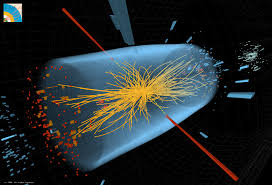
\includegraphics[height=0.6cm,width=0.8cm]{images/ppp.jpg}}
\end{picture}\put(10,2){\scriptsize\sf{Institut for theoretical physics}}\put(10,-2){\scriptsize\sf{Karlsruher institut for Technology (KIT)}}}
\cfoot{}
\rfoot{\footnotesize\sf{Thesis by Tigran Saidnia}}
\renewcommand{\headrulewidth}{0.4pt}
\renewcommand{\footrulewidth}{1.0pt}
\newcommand{\offline}{$ \overline{\textrm{\textbf{Off}}}\underline{\textrm{\textbf{line}}}\ $}


% ====================================================
% Kopf- und Fusszeile fuer "plain"-Format ueberschreiben
% ====================================================
\fancypagestyle{plain}{%
\fancyhf{}
\fancyfoot[L,C,R]{\setlength{\unitlength}{1mm}
\begin{picture}(0,0)
\put(0,-2){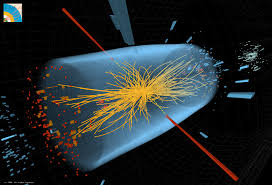
\includegraphics[height=0.6cm,width=0.8cm]{images/ppp.jpg}}
\end{picture}\put(10,2){\scriptsize\sf{Institut for theoretical physics}}\put(10,-2){\scriptsize\sf{Karlsruhe Institut of Technology (KIT)}}}
\cfoot{}
\rfoot{\footnotesize\sf{Thesis by Tigran Saidnia}}
\renewcommand{\headrulewidth}{0pt}
\renewcommand{\footrulewidth}{1.0pt}}

\begin{document}

%\doublespacing
    \parindent=0pt
    %\sloppypar
    \linespread{1.2}
    \thispagestyle{plain}
    %\frontmatter
    %\maketitle

\begin{titlepage}

\begin{center}


% Oberer Teil der Titelseite:

\includegraphics[width=0.3\textwidth]{images/Intro/kitlogo_de_rgb}\\[1cm]    

\textsc{\LARGE Master Thesis}\\[0.5cm]
\textsc{\Large by}\\[0.5cm]
\textsc{\Large Tigran Saidnia}\\[1.0cm]


% Title
\newcommand{\HRule}{\rule{\linewidth}{0.5mm}}
\HRule \\[0.8mm]
{\textbf{\Large \bfseries Emission kernels of parton showers in LO}}\\[0.8mm]

%\HRule \\[0.001mm]
%\newcommand{\HRule}{\rule{\linewidth}{0.5mm}}
%\HRule \\[0.8mm]
%{\textbf{\bfseries Emission kernels of parton showers in LO}}\\[0.8mm]

\HRule \\[1cm]
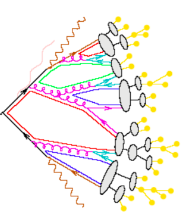
\includegraphics[scale=0.7]{images/Intro/footPicture.PNG}\\[0.8cm]   

\Large Karlsruhe institute of Technology (KIT)\\[1.5mm]
\Large Institute for theoretical physics\\[1.0cm]

{\Large Reviewer: PD Dr. Stefan Gieseke \\
\Large Second reviewer: Prof. Dr. Dieter Zeppenfeld\\
\Large External advisor: Dr. Simon Plätzer\\
\Large Advisor: Emma Simpson Dore}\\[0.8cm]   

Duration: July 1, 2018  –  July 1, 2019

\vfill

% Unterer Teil der Seite
 %\today

\end{center}

\end{titlepage}
\chapter*{}
\begin{flushleft}
\vspace{11cm}
\textbf{Statement of Originality}\\[1cm]
I hereby confirm that I have written the accompanying thesis by myself, without contributions from any sources other than those cited in the text and acknowledgements. This applies also to all graphics, drawings, maps and images included in the thesis.\\[1cm]

Karlsruhe, \today \\[1cm]
\end{flushleft}

\begin{center}
---------------------------------\\
Tigran Saidnia
\end{center}

\pagebreak

\tableofcontents
\thispagestyle{empty}
\addcontentsline{toc}{chapter}{Table of contents}
\thispagestyle{empty}
\quad
\newpage
\pagenumbering{arabic} 




\input{abstract/abtract.tex}
\newpage
\section*{Historical Background}
Knowledge is a human need. For thousands of years we have been trying to understand the secrets of the universe. Such riddles fascinated even Johann Wolfgang von Goethe, as he wrote in his book Faust \cite{goethe1921faust}; eine Tragedie, "What holds the world together in its innermost." 
Almost 400 years before Christ, an ancient Greek philosopher, Democritus, and his teacher Leukipp claimed matter can not be divided at will. Rather, there must be an Atomos (Greek: indivisible) that could no longer be subdivided.
Democritus was of the opinion that there were infinitely many atoms with different geometric forms that were in contact in a certain way. He pointed out that a thing has a color, taste or even soul, based on the apparent effect of the composition of these small grains.
\cite{capelle1968vorsokratiker}

This statement of Democritus was first laughed at by the renowned philosopher Aristotiles. It took about 2000 years for a chemist named John Dalton to deal with the subject. Based on various test series, he summarized his conclusion in his book A New System of Chemical Philosophy, that all substances consist of spherical indivisible atoms. The atoms of different elements have different masses and volumes. This was exactly the most striking difference to Democritus's atomic world.\cite{dalton2010new}

The discovery of the periodic system by D. Mendeleev and P. Meyer enabled us to arrange the atoms according to their mass in such a way that their properties occur in a certain order.\cite{haken2013atom}

In 1897 Joseph Thompson was able to obtain a stream of particles by heating metals and deflecting them by a magnetic field. This electron beam was 200 times lighter than the lightest atom, hydrogen.
His conclusion was that atoms cannot be indivisible. He suggested that each atom consists of an electrically positively charged sphere in which electrically negatively charged electrons are stored - like raisins in a cake.

Furthermore, renowned scientists as well as Marie and Pierre Curie have contributed much to the development of atomic theory by discovering radioactivity, Boltzmann by kinetic gas theory and Plank, the founder of quantum physics.
However, one of the most important steps in the atomic model was taken by the British physicist Rutherford. He bombarded a thin aluminium foil with a radioactive sample. If Thompson's cake model were correct, only a few alpha particles would be detected behind the aluminium foil. Surprisingly, many particles were visible, which could only be explained by the assumption that the majority of atoms consisted of empty spaces. Another miracle was that some particles could be seen above or below the target sample. Since it is known, the alpha particles are positively charged, it could be assumed the electric repulsive force of two positive charges. From the ideas of Planck and Rutherford, the Danish physicist Bohr (1885-1962) developed a planetary atomic model. The electrons then move around the nucleus in certain orbits, like planets orbit the sun. The orbits are also called shells. The special thing about it was that the distances of the electron orbits follow strict mathematical laws.\\  
At first, however, it remained unclear what this core should consist of. \cite{haken2013atom, demtroder2005experimentalphysik}   
In 1912, the Austrian physicist Victor Hess discovered during his balloon flights that the ionization rate of the Earth's atmosphere increases with altitude. This result was not expected because until then the Earth's radioactivity was known as the only source of air ionization. Therefore, he postulated this new type of radiation as cosmic radiation, which must originate outside the Earth's atmosphere ~\cite{Ender}.\\
Further investigations two years later confirmed the thesis of a cosmic background of such radiation. After this new discovery, it was discovered that the radiation consists of charged particles. In 1932, the American physicist Carl David Anderson was able to prove the postulated particle of Dirac, the positron, as a component of an air shower through his cloud chamber. For a long time, cosmic rays were the only way to analyse such exotic particles.\cite{Bluemer:2009zf}
This changed when particle accelerators were able to generate particles in collisions. But even today, cosmic rays are the only way to study particles of the highest energies, since these energies cannot be reached by today's particle accelerators, such as the LHC. The LHC, the world's largest accelerator at CERN, produces particles with centre-of-mass energy equivalent to a cosmic particle of nearly $10^{17} eV $, with the energy spectrum of cosmic particles reaching up to $10^{20} eV $.
However, we can only analyse such exotic particles in detail by increasing the luminosity and precision of the particle accelerators at the nucleus. 
The discovery of the neutron by Chadwick (1932) showed that atomic nuclei are made up of protons and neutrons. It was also clear that, in addition to gravitation and the electromagnetic force, there should exist two short-range forces in nature; a strong force which binds the nucleons together and a weak force which is responsible for radiation.
In the meantime it was agreed that a new theory was needed for the classification and grouping of this particle zoo. This is how the current standard model came into being.\\
The SLAC experiments indicate that the electrons can be scattered as quasi-free point-like constituents within the proton structure, which actually meant that the protons or neutrons are not point-like and must consist of other constituents. Through the bubble chamber a huge number of previously invisible particles (Gell-Mann's eightfold path) could suddenly be made visible, which represented contradictions to the previous physics. To explain this, the physicist Gell-Mann found basic building blocks from which all previously known atomic particles should be built. The components are later identified with quarks.\\
\newpage
\section*{Motivation}
For the results of particle physics experiments in connection with the strong interaction perturbation theory is used. In order to make useful and more accurate predictions, the calculations must be carried out to a higher order.\\ Simulation programs are employed for this purpose to compare experimental data with theoretical predictions. One of the most powerful tools for generating realistic collider events is the general purpose Monte Carlo (\textbf{GPMC}) event generator \cite{Buckley:2011ms}. These generators consist of different components to describe the physics in the different energy scales; hard Scattering (TeV scales) and hadronisation (GeV scales). The connection between these hard and soft ranges is established by the parton shower algorithms. To achieve higher simulation accuracy, \textbf{GPMCs} must be able to compare NNLO and higher order calculations with parton showers. Unfortunately, parton showers can not reproduce exactly the known structure of singularities present in a NNLO calculation \cite{Dasgupta:2018nvj}.
An important step for increasing the accuracy of the shower models is the incorporation of higher-order splitting functions. \\
All shower models contain kinematic to certain generate emissions in a sequence. The three major Monte Carlo programs \textbf{Pythia} \cite{Sjostrand:2006za} \cite{Sjostrand:2014zea}, \textbf{Sherpa} \cite{Gleisberg:2008ta} and \textbf{Herwig} \cite{Platzer:2009jq} \cite{Bellm:2015jjp} classify showers based on their specific choice of ordering variable.  The most common approach is to order emissions in transverse momentum.\\
 This work presents a new kinematic for the calculation of LO splitting functions. The goal is to verify the LO splitting function first and study the higher-order splitting functions in future master or even doctoral theses to a higher accuracy. The thesis begins with the Feynmann rules and colour algebra in Chapter \ref{Prerequisites} which are later used for the evaluation of the matrix elements.
Chapter \ref{Parton showers} provides a brief overview of of the general method, describing the subtraction procedure and presenting the dipole formulae. Thereafter, the kinematics in the case of massless  partons with the useful prescriptions for the matrix elements evaluation are discussed. The factorisation properties of QCD matrix elements in the soft and collinear limits for four possible parton showers due to parametrisations are outlined in Chapter \ref{LO}. The known result from the $ e^{+}e^{-} \rightarrow q \bar{q} g $ process is compared with the result of gluon radiation from a parent quark in chapters \ref{LO} and \ref{Example Applications}. \\
Chapter \ref{Summary} represents  a  summary  of  the  previous final results  that  were  obtained. Mathematical tools \ref{Math} gives more details, and some examples, of the necessary mathematical formulae for the handling of parametrisations. All detailed steps of the calculations can be found in the Appendix \ref{Appendix}.

 
\section{Old parametrisation}

	
\begin{equation}
	\left.\begin{aligned}
	&{q_i}^{\mu} = z{p_i}^{\mu} + y(1-z){p_j}^{\mu} + \sqrt{zy(1-z)}{m}_{\bot} \\
	&{q}^{\mu}   = (1-z){p_i}^{\mu} + yz {p_j}^{\mu} - \sqrt{zy(1-z)}{m}_{\bot} \\
	&{q_j}^{\mu} = (1-y) {p_j}^{\mu} \\
		&y       = \frac{q_i q}{p_i p_j} \\
&q_i +q      = p_i + yp_j \\
&q_j +q      = (1-z){p_i}^{\mu} + (1+yz-y) {p_j}^{\mu} - \sqrt{zy(1-z)}{m}_{\bot}\\
&q_i \cdot q = y(1-2z+2z^2)(p_i \cdot p_j)\\
&q_i \cdot q_j = z(1-y) (p_i \cdot p_j)\\
&q_j \cdot q = (1-z)(1-y) (p_i \cdot p_j)
		\end{aligned}
	\right\}
	\quad \text{parametrisation}
\end{equation}


\section{new kinematic}
For the general m emission case it must be defined a new mapping. The parametrisation of the splitting momenta is formalized as:
\begin{equation}
	\begin{split}
	&{k_l}^{\mu} = \alpha_l \alpha {\Lambda^{\mu}}_{\nu}{p_i}^{\nu} + y\beta{n}^{\mu} + \sqrt{y\alpha_l\beta_l}{n^{\mu}}_{\bot,l} \:\:\:\:\:\:\:\:\:\:\:\:\:\:\:{l=1,...,m} \\
	&{q_i}^{\mu}   = (1-\displaystyle\sum\limits_{l=1}^m \alpha_l) \alpha {\Lambda^{\mu}}_{\nu}{p_i}^{\nu} + y(1-\displaystyle\sum\limits_{l=1}^m \beta_l){n}^{\mu} - \sqrt{y\alpha_l\beta_l}{n^{\mu}}_{\bot,l} \\
	&{q_k}^{\mu} = \alpha {\Lambda^{\mu}}_{\nu}{p_k}^{\nu} \:\:\:\:\:\:\:\:\:\:\:\:\: {k=1,...,n}\:\:\:\:\:\:\:\:\:\:k\neq i\\
    \end{split}
\end{equation}
$ k = 1,...,n $ labels the emission momenta and is taken to be massless $ {k_l}^2 = 0 $. Where the label $ l $ denotes the count of emissions. In this work we just want to considerate the one-emission kernels. The other important issue here is that all hard momenta are on-shell, $ {p_k}^2={q_k}^2=0 $.\\
to absorb the recoil we define $ n^{\mu} $ as:

\begin{equation}
\begin{split}
{n^{\mu}} &= Q^{\mu}-\frac{Q^2}{2p_i \cdot Q} {p_i}^{\mu}
\end{split}	
\end{equation}

Whereby Q is the total momentum with:

\begin{equation}
\begin{split}	
{Q}^{\mu} &= {q_i}^{\mu}+\displaystyle\sum\limits_{l=1}^m k_l^{\mu}+\displaystyle\sum\limits_{k=1}^m q_k^{\mu}={p_i}^{\mu}+\displaystyle\sum\limits_{k=1}^m p_k^{\mu}
\end{split}	
\end{equation}
To fulfil the condition that the emission momenta are massless, we need the following condition:

\begin{equation}
\begin{split}
	{n^{\mu}}_{\bot,l}{\Lambda^{\mu}}_{\nu}{p_i}^{\nu} &= {n_{\bot,l}} \cdot n = {n_{\bot,l}} \cdot Q =0\\
	{n^{\mu}}_{\bot,l}\cdot p_k &\neq0\\
\end{split}	
\end{equation}

$ {n}^2_{\bot,l} = -2\alpha{\Lambda^{\mu}}_{\nu}{p_i}^{\nu} n_{\mu} $ is not on-shell and in terms of single emission case we get $ {n}^2_{\bot,1} = -2p_i\cdot Q $.
The parameter y is related to the virtuality of the splitting parton:

\begin{equation}
\begin{split}
{q_i}^{\mu} +\displaystyle\sum\limits_{l=1}^m k_l^{\mu}   &= \alpha{\Lambda^{\mu}}_{\nu}{p_i}^{\nu} +y{n}^{\mu}\\
    \end{split}
\end{equation}
With $ \alpha = \sqrt{1-y} $.
\subsubsection*{Lorenz trafo}
In order to be able to work with the parametrisation, we have to do the Lorenz transformation of the Emitters, Spectator and total momentum first.

\begin{equation}
\begin{split}	
&\alpha{\Lambda^{\mu}}_{\nu} = {p_i}^{\mu} p_{i\nu} \frac{-y^2 Q^2}{4(p_i\cdot Q)^2(1+\sqrt{1-y}-\frac{y}{2})}
+{p_i}^{\mu} Q_{\nu} \frac{y(1+\sqrt{1-y})}{2(p_i\cdot Q)(1+\sqrt{1-y}-\frac{y}{2})}\\
&+{Q}^{\mu} p_{i\nu} \frac{(y^2 -y-y\sqrt{1-y})}{2(p_i\cdot Q)(1+\sqrt{1-y}-\frac{y}{2})}+\sqrt{1-y} {\eta^{\mu}}_{\nu}\\
\end{split}
\end{equation}

In the collinear limit of $ y \rightarrow 0, \alpha \rightarrow 1 $
this transformation reduces to trivial $ {\eta^{\mu}}_{\nu} $.


\begin{equation}
\begin{split}
&{\hat{{p_i}}}^{\mu}=\alpha{\Lambda^{\mu}}_{\nu} {p_i}^{\nu}= {p_i}^{\mu} p_{i\nu}{p_i}^{\nu} \frac{-y^2 Q^2}{4(p_i\cdot Q)^2(1+\sqrt{1-y}-\frac{y}{2})}
	+{p_i}^{\mu} Q_{\nu}{p_i}^{\nu} \frac{y(1+\sqrt{1-y})}{2(p_i\cdot Q)(1+\sqrt{1-y}-\frac{y}{2})}\\
&+{Q}^{\mu} p_{i\nu}{p_i}^{\nu} \frac{(y^2 -y-y\sqrt{1-y})}{2(p_i\cdot Q)(1+\sqrt{1-y}-\frac{y}{2})}+\sqrt{1-y} {\eta^{\mu}}_{\nu}{p_i}^{\nu}\\
\end{split}
\end{equation}

\begin{equation}
\begin{split}
&{\hat{{p_i}}}^{\mu}={p_i}^{\mu} (Q\cdot p_i) \frac{y(1+\sqrt{1-y})}{2(p_i\cdot Q)(1+\sqrt{1-y}-\frac{y}{2})}+\sqrt{1-y} {p_i}^{\mu}\\
&={p_i}^{\mu} [ \frac{y(1+\sqrt{1-y})}{(2+2\sqrt{1-y}-y)}+\sqrt{1-y}]={p_i}^{\mu}
    \end{split}
\end{equation}

\begin{equation}
	\begin{aligned}
		\fbox{$  {\hat{{p_i}}}^{\mu}=\alpha{\Lambda^{\mu}}_{\nu} {p_i}^{\nu}= {p_i}^{\mu}$}
    \end{aligned}
\end{equation}

\begin{equation}
	\begin{aligned}
	{\hat{{p_k}}}^{\mu}=\alpha{\Lambda^{\mu}}_{\nu} {p_k}^{\nu}= {p_i}^{\mu} p_{i\nu}{p_k}^{\nu} \frac{-y^2 Q^2}{4(p_i\cdot Q)^2(1+\sqrt{1-y}-\frac{y}{2})}
	+{p_i}^{\mu} Q_{\nu}{p_k}^{\nu} \frac{y(1+\sqrt{1-y})}{2(p_i\cdot Q)(1+\sqrt{1-y}-\frac{y}{2})}\\
	+{Q}^{\mu} p_{i\nu}{p_k}^{\nu} \frac{(y^2 -y-y\sqrt{1-y})}{2(p_i\cdot Q)(1+\sqrt{1-y}-\frac{y}{2})}+\sqrt{1-y} {\eta^{\mu}}_{\nu}{p_k}^{\nu}\\
    \end{aligned}
\end{equation}

\begin{equation}
	\begin{aligned}
	{\hat{{p_k}}}^{\mu}=\alpha{\Lambda^{\mu}}_{\nu} {p_k}^{\nu}= {p_i}^{\mu}[  \frac{-y^2 Q^2 (p_{i}\cdot {p_k})}{4(p_i\cdot Q)^2(1+\sqrt{1-y}-\frac{y}{2})}+ \frac{y(1+\sqrt{1-y})(Q \cdot {p_k})}{2(p_i\cdot Q)(1+\sqrt{1-y}-\frac{y}{2})}]\\
	+{Q}^{\mu} [ \frac{(y^2 -y-y\sqrt{1-y}) (p_{i}\cdot {p_k})}{2(p_i\cdot Q)(1+\sqrt{1-y}-\frac{y}{2})}]
	+\sqrt{1-y} {p_k}^{\mu}\\
    \end{aligned}
\end{equation}


\begin{equation}
	\begin{aligned}
	{\hat{{p_k}}}^{\mu}&=\alpha{\Lambda^{\mu}}_{\nu} {p_k}^{\nu}= {p_i}^{\mu}[  \frac{-y^2 Q^2 (p_{i}\cdot {p_k})}{4(p_i\cdot Q)^2(1+\sqrt{1-y}-\frac{y}{2})}+ \frac{y(1+\sqrt{1-y})(Q \cdot {p_k})}{2(p_i\cdot Q)(1+\sqrt{1-y}-\frac{y}{2})}]\\
	&+{Q}^{\mu} [ \frac{(y^2 -y-y\sqrt{1-y}) (p_{i}\cdot {p_k})}{2(p_i\cdot Q)(1+\sqrt{1-y}-\frac{y}{2})}]+\sqrt{1-y} {p_k}^{\mu}\\	
\text{with}\\
	A_1 &\equiv  \frac{-y^2 Q^2 (p_{i}\cdot {p_k})}{4(p_i\cdot Q)^2(1+\sqrt{1-y}-\frac{y}{2})}+ \frac{y(1+\sqrt{1-y})(Q \cdot {p_k})}{2(p_i\cdot Q)(1+\sqrt{1-y}-\frac{y}{2})}\\
		A_2 &\equiv   \frac{(y^2 -y-y\sqrt{1-y}) (p_{i}\cdot {p_k})}{2(p_i\cdot Q)(1+\sqrt{1-y}-\frac{y}{2})}\:\:\:\:\:\:\:\:\:\:\:\:\:\:\:\:\:\:\:\:\:\:\:\:\:\:\:\:\:\:\:\:\:\:\:\:\:\:\:\:\:\:\:\:\:\:\:\:\:\:\:\:\:\:\\\
    \end{aligned}    
\end{equation}
\begin{equation}
	\begin{aligned}
		\fbox{$  {\hat{{p_k}}}^{\mu}= A_1 \:{p_i}^{\mu}+A_2\:{Q}^{\mu}+\sqrt{1-y} {p_k}^{\mu} $}
    \end{aligned}
\end{equation}


\begin{equation}
	\begin{aligned}
	{\hat{{Q}}}^{\mu}&=\alpha{\Lambda^{\mu}}_{\nu} {Q}^{\nu}= {p_i}^{\mu}[  \frac{-y^2 Q^2 (p_{i}\cdot {Q})}{4(p_i\cdot Q)^2(1+\sqrt{1-y}-\frac{y}{2})}+ \frac{y(1+\sqrt{1-y})Q^2}{2(p_i\cdot Q)(1+\sqrt{1-y}-\frac{y}{2})}]\\
	&+{Q}^{\mu} [ \frac{(y^2 -y-y\sqrt{1-y}) (p_{i}\cdot {Q})}{2(p_i\cdot Q)(1+\sqrt{1-y}-\frac{y}{2})}]
	+\sqrt{1-y} {Q}^{\mu}\\
\text{with}\\
	S_1 &\equiv  \frac{Q^2}{2p_i \cdot Q}[\frac{-y^2}{2(1+\sqrt{1-y}-\frac{y}{2})}+ \frac{y(1+\sqrt{1-y})}{(1+\sqrt{1-y}-\frac{y}{2})}]=\frac{Q^2}{2p_i \cdot Q}y\\
		S_2 &\equiv   \frac{(y^2 -y-y\sqrt{1-y})}{2(1+\sqrt{1-y}-\frac{y}{2})}+\sqrt{1-y}=1-y\:\:\:\:\:\:\:\:\:\:\:\:\:\:\:\:\:\:\:\:\:\:\:\:\:\:\:\:\:\:\:\:\:\:\:\:\:\:\:\:\:\:\:\:\:\:\:\:\:\:\:\:\:\:\\\	
    \end{aligned}    
\end{equation}
\begin{equation}
	\begin{aligned}
		\fbox{$  {\hat{{Q}}}^{\mu}= \frac{Q^2}{2p_i \cdot Q}y \:{p_i}^{\mu}+(1-y)\:{Q}^{\mu} $}
    \end{aligned}
\end{equation}

\section{Single emission part}
\begin{equation}
	\begin{aligned}
	{k_1}^{\mu} &= (\alpha_1 -y\beta_1(\frac{Q^2}{2p_i \cdot Q})) {p_i}^{\mu} + y\beta_1{Q}^{\mu} + \sqrt{y\alpha_1\beta_1}{n^{\mu}}_{\bot,1}  \\
	{q_i}^{\mu}   &= (\beta_1 -\alpha_1 y(\frac{Q^2}{2p_i \cdot Q})){p_i}^{\mu} + y\alpha_1{Q}^{\mu} - \sqrt{y\alpha_1\beta_1}{n^{\mu}}_{\bot,l} \\
	{q_k}^{\mu} &= \alpha {\Lambda^{\mu}}_{\nu}{p_k}^{\nu} \:\:\:\:\:\:\:\:\:\:\:\:\: {k=1,...,n}\:\:\:\:\:\:\:\:\:\:k\neq i\\
	\\
	\\
		{k_1}^{\mu} &= \zeta_1 {p_i}^{\mu} + \lambda_1{Q}^{\mu} + \sqrt{y\alpha_1\beta_1}{n^{\mu}}_{\bot,1}  \\
	{q_i}^{\mu}   &= \zeta_q{p_i}^{\mu} + \lambda_q{Q}^{\mu} - \sqrt{y\alpha_1\beta_1}{n^{\mu}}_{\bot,l} \\
	{q_k}^{\mu} &= A_1{p_i}^{\mu} + A_2{Q}^{\mu} + \sqrt{1-y}{p_k^{\mu}}\\
    \end{aligned}
\end{equation}

\begin{equation}
	\begin{aligned}
	\zeta_1\zeta_1=({\alpha_1}^2 -2y\alpha_1 \beta_1(\frac{Q^2}{2p_i \cdot Q})+y^2{\beta_1}^2(\frac{Q^2}{2p_i \cdot Q})^2)\\
	\zeta_1\lambda_1=(y\alpha_1\beta_1 -{y^2\beta_1}^2(\frac{Q^2}{2p_i \cdot Q}))\\
	\zeta_1\zeta_q=(\alpha_1\beta_1-y({\alpha_1}^2+{\beta_1}^2) (\frac{Q^2}{2p_i \cdot Q})+y^2{\alpha_1}{\beta_1}(\frac{Q^2}{2p_i \cdot Q})^2)\\
	\zeta_1\lambda_q=(y{\alpha_1}^2 -y^2\beta_1\alpha_1(\frac{Q^2}{2p_i \cdot Q}))\\
	\zeta_q\zeta_q=	({\beta_1}^2 -2y\alpha_1\beta_1 (\frac{Q^2}{2p_i \cdot Q})+ y^2{\alpha_1}^2 (\frac{Q^2}{2p_i \cdot Q})^2) \\
	\zeta_q\lambda_1=(y{\beta_1}^2 -y^2\alpha_1 \beta_1(\frac{Q^2}{2p_i \cdot Q}))\\
	\zeta_q\zeta_1=(\beta_1\alpha_1-y({\beta_1}^2+{\alpha_1}^2)(\frac{Q^2}{2p_i \cdot Q})+y^2\alpha_1\beta_1 (\frac{Q^2}{2p_i \cdot Q})^2)\\
	\zeta_q\lambda_q=(y\beta_1\alpha_1 -y^2{\alpha_1}^2(\frac{Q^2}{2p_i \cdot Q}))\\
	\lambda_1\lambda_1=y^2{\beta_1}^2\\
	\lambda_1\zeta_q=(y{\beta_1}^2 -y^2\alpha_1 \beta_1(\frac{Q^2}{2p_i \cdot Q}))\\
	\lambda_1\lambda_q=y^2\beta_1\alpha_1\\
	\lambda_1\zeta_1=(y\beta_1\alpha_1 -y^2{\beta_1}^2(\frac{Q^2}{2p_i \cdot Q}))\\
	\lambda_q\lambda_q=y^2{\alpha_1}^2\\
	\lambda_q\lambda_1=y^2\alpha_1\beta_1\\
	\lambda_q\zeta_q=(y\alpha_1\beta_1 -y^2{\alpha_1}^2 (\frac{Q^2}{2p_i \cdot Q}))\\
	\lambda_q\zeta_1=(y{\alpha_1}^2 -y^2\alpha_1\beta_1(\frac{Q^2}{2p_i \cdot Q}))
    \end{aligned}
\end{equation}
\section{Common scalar products}
\begin{equation}
	\begin{aligned}	
k_1 \cdot q_i &= (\zeta_1 \lambda_q + \lambda_1 \zeta_q)p_i \cdot Q+\lambda_1 \lambda_q Q^2 -y\alpha_1\beta_1 {n^{2}}_{\bot,1}\\
	&=[(\alpha_1 -y\beta_1(\frac{Q^2}{2p_i \cdot Q}))y\alpha_1+y\beta_1(\beta_1 -\alpha_1 y(\frac{Q^2}{2p_i \cdot Q}))]\:p_i \cdot Q\\
	&\:\:\:\:\:\:\:y^2\beta_1\alpha_1\: Q^2+2y\alpha_1\beta_1\:p_iQ\\
\Rightarrow	k_1 \cdot q_i &=[y{\alpha_1}^2 -y^2\alpha_1\beta_1(\frac{Q^2}{2p_i \cdot Q})+y {\beta_1}^2-y^2\alpha_1\beta_1(\frac{Q^2}{2p_i \cdot Q})]\:p_i\cdot Q\\
	&y^2\beta_1\alpha_1\: Q^2+2y\alpha_1\beta_1\:p_iQ\\	
    \end{aligned}
\end{equation}

\begin{equation}
	\begin{aligned}
		\fbox{$  k_1 \cdot q_i=y({\alpha_1}+\beta_1)^2\:p_i\cdot Q = y\:p_i\cdot Q $}
    \end{aligned}
\end{equation}

\begin{equation}
	\begin{aligned}	
	k_1 \cdot q_k &= (\zeta_1 A_2 + \lambda_1 A_1)p_i \cdot Q+\zeta_1 \sqrt{1-y}\:p_i\cdot p_k + \lambda_1 A_2\:Q^2+ \lambda_1\sqrt{1-y}\:Q\cdot p_k\\
	&+\sqrt{\alpha_1\beta_1y(1-y)} p_k \cdot {n_{\bot,1}}\\	
	&=\lbrace[(\alpha_1 -y\beta_1(\frac{Q^2}{2p_i \cdot Q}))\frac{(y^2 -y-y\sqrt{1-y}) (p_{i}\cdot {p_k})}{2(p_i\cdot Q)(1+\sqrt{1-y}-\frac{y}{2})}]\\&
	+y\beta_1[\frac{-y^2 Q^2 (p_{i}\cdot {p_k})}{4(p_i\cdot Q)^2(1+\sqrt{1-y}-\frac{y}{2})}+ \frac{y(1+\sqrt{1-y})(Q \cdot {p_k})}{2(p_i\cdot Q)(1+\sqrt{1-y}-\frac{y}{2})}]\rbrace\:p_i \cdot Q\\
	&+(\alpha_1 -y\beta_1(\frac{Q^2}{2p_i \cdot Q}))\sqrt{1-y}\:p_i \cdot p_k+y\beta_1\frac{(y^2 -y-y\sqrt{1-y}) (p_{i}\cdot {p_k})}{2(p_i\cdot Q)(1+\sqrt{1-y}-\frac{y}{2})}Q^2\\
	&+y\beta_1\sqrt{1-y} Q\cdot p_k+\sqrt{\alpha_1\beta_1y(1-y)} p_k \cdot {n_{\bot,1}} 
    \end{aligned}
\end{equation}

\begin{equation}
	\begin{aligned}
	k_1 \cdot q_k &= \alpha_1 \frac{(y^2 -y-y\sqrt{1-y}) }{2(1+\sqrt{1-y}-\frac{y}{2})}(p_{i}\cdot {p_k})
	-y\beta_1(\frac{Q^2}{2p_i \cdot Q})\frac{(y^2 -y-y\sqrt{1-y})}{2(1+\sqrt{1-y}-\frac{y}{2})}(p_{i}\cdot {p_k})\\
&+y\beta_1\frac{-y^2 Q^2 }{4(p_i\cdot Q)(1+\sqrt{1-y}-\frac{y}{2})}(p_{i}\cdot {p_k})+ y\beta_1\frac{y(1+\sqrt{1-y})}{2(1+\sqrt{1-y}-\frac{y}{2})}\:Q \cdot p_k\\
	&+\alpha_1 \sqrt{1-y}\:p_i \cdot p_k-y\beta_1(\frac{Q^2}{2p_i \cdot Q})\sqrt{1-y}\:p_i \cdot p_k\\
	&+y\beta_1(\frac{Q^2}{2p_i \cdot Q})\frac{(y^2 -y-y\sqrt{1-y})}{2(1+\sqrt{1-y}-\frac{y}{2})}(p_{i}\cdot {p_k})+y\beta_1\sqrt{1-y}(Q\cdot p_k)\\
	&+\sqrt{\alpha_1\beta_1y(1-y)} p_k \cdot {n_{\bot,1}} 
    \end{aligned}
\end{equation}

\begin{equation}
	\begin{aligned}
	k_1 \cdot q_k &= [\alpha_1 \frac{(y^2 -y-y\sqrt{1-y}) }{2(1+\sqrt{1-y}-\frac{y}{2})}+y\beta_1\frac{-y^2 Q^2 }{4(p_i\cdot Q)(1+\sqrt{1-y}-\frac{y}{2})}+\alpha_1 \sqrt{1-y}\\&-y\beta_1(\frac{Q^2}{2p_i \cdot Q})\sqrt{1-y}]\:p_i \cdot p_k+[y\beta_1\frac{y(1+\sqrt{1-y})}{2(1+\sqrt{1-y}-\frac{y}{2})}+y\beta_1\sqrt{1-y}](Q\cdot p_k)\\
	&+\sqrt{\alpha_1\beta_1y(1-y)} p_k \cdot {n_{\bot,1}} 
    \end{aligned}
\end{equation}

\begin{equation}
	\begin{aligned}
	k_1 \cdot q_k &= \lbrace\alpha_1 [\frac{(y^2 -y-y\sqrt{1-y}) }{2(1+\sqrt{1-y}-\frac{y}{2})}+ \sqrt{1-y}]\\
	&+y\beta_1(\frac{Q^2}{p_i \cdot Q})[\frac{-y^2 }{4(1+\sqrt{1-y}-\frac{y}{2})}-\sqrt{1-y}]\rbrace\:p_i \cdot p_k\\
	&+y\beta_1[\frac{y(1+\sqrt{1-y})}{2(1+\sqrt{1-y}-\frac{y}{2})}+\sqrt{1-y}](Q\cdot p_k)\\
	&+\sqrt{\alpha_1\beta_1y(1-y)} p_k \cdot {n_{\bot,1}} 
    \end{aligned}
\end{equation}

\begin{equation}
	\begin{aligned}
		\fbox{$  k_1 \cdot q_k = [\alpha_1 (1-y)+y\beta_1(\frac{Q^2}{2p_i \cdot Q})]\:p_i \cdot p_k+y\beta_1\:Q\cdot p_k+\sqrt{\alpha_1\beta_1y(1-y)} p_k \cdot {n_{\bot,1}} $}
    \end{aligned}
\end{equation}

\begin{equation}
	\begin{aligned}	
	q_i \cdot q_k &= (\zeta_q A_2 + \lambda_q A_1)p_i \cdot Q+\zeta_q \sqrt{1-y}\:p_i\cdot p_k + \lambda_q A_2\:Q^2+ \lambda_q\sqrt{1-y}\:Q\cdot p_k\\
	&-\sqrt{\alpha_1\beta_1y(1-y)} p_k \cdot {n_{\bot,1}}\\	
	&=\lbrace[(\beta_1 -y\alpha_1(\frac{Q^2}{2p_i \cdot Q}))\frac{(y^2 -y-y\sqrt{1-y}) (p_{i}\cdot {p_k})}{2(p_i\cdot Q)(1+\sqrt{1-y}-\frac{y}{2})}]\\&
	+y\alpha_1[\frac{-y^2 Q^2 (p_{i}\cdot {p_k})}{4(p_i\cdot Q)^2(1+\sqrt{1-y}-\frac{y}{2})}+ \frac{y(1+\sqrt{1-y})(Q \cdot {p_k})}{2(p_i\cdot Q)(1+\sqrt{1-y}-\frac{y}{2})}]\rbrace\:p_i \cdot Q\\
	&+(\beta_1 -y\alpha_1(\frac{Q^2}{2p_i \cdot Q}))\sqrt{1-y}\:p_i \cdot p_k+y\alpha_1\frac{(y^2 -y-y\sqrt{1-y}) (p_{i}\cdot {p_k})}{2(p_i\cdot Q)(1+\sqrt{1-y}-\frac{y}{2})}Q^2\\
	&+y\alpha_1\sqrt{1-y} Q\cdot p_k-\sqrt{\alpha_1\beta_1y(1-y)} p_k \cdot {n_{\bot,1}} 
    \end{aligned}
\end{equation}


\begin{equation}
	\begin{aligned}
	q_i \cdot q_k &= \beta_1 \frac{(y^2 -y-y\sqrt{1-y}) }{2(1+\sqrt{1-y}-\frac{y}{2})}(p_{i}\cdot {p_k})
	-y\alpha_1(\frac{Q^2}{2p_i \cdot Q})\frac{(y^2 -y-y\sqrt{1-y})}{2(1+\sqrt{1-y}-\frac{y}{2})}(p_{i}\cdot {p_k})\\
&+y\alpha_1\frac{-y^2 Q^2 }{4(p_i\cdot Q)(1+\sqrt{1-y}-\frac{y}{2})}(p_{i}\cdot {p_k})+ y\alpha_1\frac{y(1+\sqrt{1-y})}{2(1+\sqrt{1-y}-\frac{y}{2})}\:Q \cdot p_k\\
	&+\beta_1 \sqrt{1-y}\:p_i \cdot p_k-y\alpha_1(\frac{Q^2}{2p_i \cdot Q})\sqrt{1-y}\:p_i \cdot p_k\\
	&+y\alpha_1(\frac{Q^2}{2p_i \cdot Q})\frac{(y^2 -y-y\sqrt{1-y})}{2(1+\sqrt{1-y}-\frac{y}{2})}(p_{i}\cdot {p_k})+y\alpha_1\sqrt{1-y}(Q\cdot p_k)\\
	&-\sqrt{\alpha_1\beta_1y(1-y)} p_k \cdot {n_{\bot,1}} 
    \end{aligned}
\end{equation}

\begin{equation}
	\begin{aligned}
	q_i \cdot q_k &= [\beta_1 \frac{(y^2 -y-y\sqrt{1-y}) }{2(1+\sqrt{1-y}-\frac{y}{2})}+y\alpha_1\frac{-y^2 Q^2 }{4(p_i\cdot Q)(1+\sqrt{1-y}-\frac{y}{2})}+\beta_1 \sqrt{1-y}\\&-y\alpha_1(\frac{Q^2}{2p_i \cdot Q})\sqrt{1-y}]\:p_i \cdot p_k+[y\alpha_1\frac{y(1+\sqrt{1-y})}{2(1+\sqrt{1-y}-\frac{y}{2})}+y\alpha_1\sqrt{1-y}](Q\cdot p_k)\\
	&-\sqrt{\alpha_1\beta_1y(1-y)} p_k \cdot {n_{\bot,1}} 
    \end{aligned}
\end{equation}

\begin{equation}
	\begin{aligned}
	k_1 \cdot q_k &= \lbrace\beta_1 [\frac{(y^2 -y-y\sqrt{1-y}) }{2(1+\sqrt{1-y}-\frac{y}{2})}+ \sqrt{1-y}]\\
	&+y\alpha_1(\frac{Q^2}{p_i \cdot Q})[\frac{-y^2 }{4(1+\sqrt{1-y}-\frac{y}{2})}-\sqrt{1-y}]\rbrace\:p_i \cdot p_k\\
	&+y\alpha_1[\frac{y(1+\sqrt{1-y})}{2(1+\sqrt{1-y}-\frac{y}{2})}+\sqrt{1-y}](Q\cdot p_k)\\
	&-\sqrt{\alpha_1\beta_1y(1-y)} p_k \cdot {n_{\bot,1}} 
    \end{aligned}
\end{equation}

\begin{equation}
	\begin{aligned}
		\fbox{$  q_i \cdot q_k = [\beta_1 (1-y)+y\alpha_1(\frac{Q^2}{2p_i \cdot Q})]\:p_i \cdot p_k+y\alpha_1\:Q\cdot p_k-\sqrt{\alpha_1\beta_1y(1-y)} p_k \cdot {n_{\bot,1}} $}
    \end{aligned}
\end{equation}

\section{Parametrization in terms of $ (k_1 \cdot q_i )(k_1 \cdot q_k) $}
\begin{equation}
	\begin{aligned}
		\fbox{$  (k_1 \cdot q_i )(k_1 \cdot q_k) {\color[RGB]{255,0,0} \: \approx\:} y(1-\beta_1) (1-y)\:(p_i \cdot p_k)(p_i \cdot Q) $}
    \end{aligned}
\end{equation}

\begin{equation}
\begin{split}
{k_1}^{{\eta}}{k_1}^{{\eta}^{\prime}}&=[(1-\beta_1)^2-y^2 {\beta_1}^2 (\frac{Q^2}{2p_i \cdot Q})^2] {p_i}^{{\eta}}{p_i}^{{\eta}^{\prime}}-y^2 {\beta_1}^2 (\frac{Q^2}{2p_i \cdot Q}){p_i}^{{\eta}}{Q}^{{\eta}^{\prime}}-y^2 {\beta_1}^2 (\frac{Q^2}{2p_i \cdot Q}){Q}^{{\eta}}{p_i}^{{\eta}^{\prime}}\\
{k_1}^{{\eta}}{q_i}^{{\eta}^{\prime}}&=[\beta_1(1-\beta_1)-y {\beta_1}^2 (\frac{Q^2}{2p_i \cdot Q})] {p_i}^{{\eta}}{p_i}^{{\eta}^{\prime}}+y {\beta_1}^2 {Q}^{{\eta}}{p_i}^{{\eta}^{\prime}}\\
{q_i}^{{\eta}}{k_1}^{{\eta}^{\prime}}&=[\beta_1(1-\beta_1)-y {\beta_1}^2 (\frac{Q^2}{2p_i \cdot Q})] {p_i}^{{\eta}}{p_i}^{{\eta}^{\prime}}+y {\beta_1}^2 {p_i}^{{\eta}}{Q}^{{\eta}^{\prime}}\\
{q_i}^{{\eta}}{q_i}^{{\eta}^{\prime}}&={\beta_1}^2 {p_i}^{{\eta}}{p_i}^{{\eta}^{\prime}}\\
{k_1}^{{\eta}}{q_k}^{{\eta}^{\prime}}&= [(1-\beta_1)-y\beta_1 (\frac{Q^2}{2p_i \cdot Q})] \sqrt{1-y}{p_i}^{{\eta}}{{p_k}^{{\eta}^{\prime}}}-y {\beta_1} (\frac{Q^2}{2p_i \cdot Q}) A_1 \:{p_i}^{{\eta}}{p_i}^{{\eta}^{\prime}}
-y {\beta_1} (\frac{Q^2}{2p_i \cdot Q}) A_2\: {p_i}^{{\eta}}{Q}^{{\eta}^{\prime}}\\
&+y {\beta_1} A_1 \:{Q}^{{\eta}}{p_i}^{{\eta}^{\prime}}+y {\beta_1} A_2 \:{Q}^{{\eta}}{Q}^{{\eta}^{\prime}}+y {\beta_1}\sqrt{1-y}{Q}^{{\eta}}{{p_k}^{{\eta}^{\prime}}}\\
{q_i}^{{\eta}}{q_k}^{{\eta}^{\prime}}&=A_1\beta_1 {p_i}^{{\eta}}{{p_i}^{{\eta}^{\prime}}}+A_2\beta_1 {p_i}^{{\eta}}{{Q}^{{\eta}^{\prime}}}+\beta_1 \sqrt{1-y}{p_i}^{{\eta}}{{p_k}^{{\eta}^{\prime}}}\\
{q_k}^{\eta}{k_1}^{{{\eta}}^{\prime}}&=[(1-\beta_1)-y\beta_1 (\frac{Q^2}{2p_i \cdot Q})] \sqrt{1-y}{p_k}^{{\eta}}{{p_i}^{{\eta}^{\prime}}}-y {\beta_1} (\frac{Q^2}{2p_i \cdot Q}) A_1 \:{p_i}^{{\eta}}{p_i}^{{\eta}^{\prime}}
-y {\beta_1} (\frac{Q^2}{2p_i \cdot Q}) A_2\: {Q}^{{\eta}}{p_i}^{{\eta}^{\prime}}\\
&+y {\beta_1} A_1 \:{p_i}^{{\eta}}{Q}^{{\eta}^{\prime}}+y {\beta_1} A_2 \:{Q}^{{\eta}}{Q}^{{\eta}^{\prime}}+y {\beta_1}\sqrt{1-y}{p_k}^{{\eta}}{{Q}^{{\eta}^{\prime}}}\\
{q_k}^{\eta}{q_i}^{{{\eta}}^{\prime}}&=A_1\beta_1 {p_i}^{{\eta}}{{p_i}^{{\eta}^{\prime}}}+A_2\beta_1 {Q}^{{\eta}}{{p_i}^{{\eta}^{\prime}}}+\beta_1 \sqrt{1-y}{p_k}^{{\eta}}{{p_i}^{{\eta}^{\prime}}}\\
\end{split}
\end{equation}

\section{Parametrization in terms of $ (k_1 \cdot q_i )(k_1 \cdot q_i) $}
\begin{equation}
	\begin{aligned}
		\fbox{$  (k_1 \cdot q_i )(k_1 \cdot q_i)  = y^2(p_i \cdot Q)(p_i \cdot Q) $}
    \end{aligned}
\end{equation}

\begin{equation}
\begin{split}
{k_1}^{{\eta}}{k_1}^{{\eta}^{\prime}}&=[(1-\beta_1)^2-2y {\beta_1} (\frac{Q^2}{2p_i \cdot Q})] {p_i}^{{\eta}}{p_i}^{{\eta}^{\prime}}+y {\beta_1}(1-\beta_1) (\frac{Q^2}{2p_i \cdot Q}){p_i}^{{\eta}}{Q}^{{\eta}^{\prime}}+y {\beta_1}(1-\beta_1) (\frac{Q^2}{2p_i \cdot Q}){Q}^{{\eta}}{p_i}^{{\eta}^{\prime}}\\
{k_1}^{{\eta}}{q_i}^{{\eta}^{\prime}}&=[\beta_1(1-\beta_1)-y (1-{\beta_1})^2 (\frac{Q^2}{2p_i \cdot Q})-y {\beta_1}^2 (\frac{Q^2}{2p_i \cdot Q})] {p_i}^{{\eta}}{p_i}^{{\eta}^{\prime}}+y (1-\beta_1)^2 {Q}^{{\eta}}{p_i}^{{\eta}^{\prime}}\\
{q_i}^{{\eta}}{k_1}^{{\eta}^{\prime}}&=[\beta_1(1-\beta_1)-y (1-{\beta_1})^2 (\frac{Q^2}{2p_i \cdot Q})-y {\beta_1}^2 (\frac{Q^2}{2p_i \cdot Q})] {p_i}^{{\eta}}{p_i}^{{\eta}^{\prime}}+y (1-\beta_1)^2 {p_i}^{{\eta}}{Q}^{{\eta}^{\prime}}\\
{q_i}^{{\eta}}{q_i}^{{\eta}^{\prime}}&=[{\beta_1}^2 -2y \beta_1 (1-{\beta_1}) (\frac{Q^2}{2p_i \cdot Q})]{p_i}^{{\eta}}{p_i}^{{\eta}^{\prime}}+y {\beta_1}(1-\beta_1) (\frac{Q^2}{2p_i \cdot Q}){p_i}^{{\eta}}{Q}^{{\eta}^{\prime}}+y {\beta_1}(1-\beta_1) (\frac{Q^2}{2p_i \cdot Q}){Q}^{{\eta}}{p_i}^{{\eta}^{\prime}}\\
{k_1}^{{\eta}}{q_k}^{{\eta}^{\prime}}&= (1-\beta_1)A_1{p_i}^{{\eta}}{{p_i}^{{\eta}^{\prime}}}+(1-\beta_1)A_2{p_i}^{{\eta}}{{Q}^{{\eta}^{\prime}}}+(1-\beta_1)\sqrt{1-y}{p_i}^{{\eta}}{{p_k}^{{\eta}^{\prime}}}\\
{q_i}^{{\eta}}{q_k}^{{\eta}^{\prime}}&=A_1\beta_1 {p_i}^{{\eta}}{{p_i}^{{\eta}^{\prime}}}+A_2\beta_1 {p_i}^{{\eta}}{{Q}^{{\eta}^{\prime}}}+\beta_1 \sqrt{1-y}{p_i}^{{\eta}}{{p_k}^{{\eta}^{\prime}}}\\
{q_k}^{\eta}{k_1}^{{{\eta}}^{\prime}}&=(1-\beta_1)A_1{p_i}^{{\eta}}{{p_i}^{{\eta}^{\prime}}}+(1-\beta_1)A_2{Q}^{{\eta}}{{p_i}^{{\eta}^{\prime}}}+(1-\beta_1)\sqrt{1-y}{p_k}^{{\eta}}{{p_i}^{{\eta}^{\prime}}}\\
{q_k}^{\eta}{q_i}^{{{\eta}}^{\prime}}&=A_1\beta_1 {p_i}^{{\eta}}{{p_i}^{{\eta}^{\prime}}}+A_2\beta_1 {Q}^{{\eta}}{{p_i}^{{\eta}^{\prime}}}+\beta_1 \sqrt{1-y}{p_k}^{{\eta}}{{p_i}^{{\eta}^{\prime}}}\\
\end{split}
\end{equation}
\newpage
\section{Altarelli-Parisi splitting functions}

	
\begin{equation}
	\left.\begin{aligned}
\langle\:\hat{P_{qq}}\rangle &= C_F[\frac{1+z^2}{1-z}-\varepsilon(1-z)]\\
\langle\:\hat{P_{gq}}\rangle &= T_R[1-\frac{2z(1-z)}{1-\varepsilon}]\\
\langle\:\hat{P_{qg}}\rangle &= C_F[\frac{1+(1-z)^2}{z}-\varepsilon z]\\
\langle\:\hat{P_{gg}}\rangle &= 2C_A[\frac{z}{1-z}+\frac{1-z}{z}+z(1-z)]
\end{aligned}
	\right\}
	\quad \text{splitting functions}
\end{equation}

\newpage
\section{Colour factor calculation}
fundamental representation in $ SU(2) $ and $ SU(3) $
\begin{equation}
\begin{split}
T^a = \tau^a \equiv \frac{\sigma ^2}{2}\:\:\:\:\:\:\: \mathit{with\: Pauli\: matrices\: \sigma ^a}\\
T^a = \vartheta^a \equiv \frac{\lambda ^2}{2} \:\:\:\:\:\:\: \mathit{with\: Gell-Mann\: matrices\: \lambda ^a}
\end{split}
\end{equation}

\begin{equation}
\begin{split}
\lambda ^1 =\begin{pmatrix} 0& 1 &\\ 1& 0 &\\ & & 0 \end{pmatrix},\:\:\: \lambda ^2 =\begin{pmatrix} 0& -i &\\ i& 0 &\\ & & 0 \end{pmatrix}, 
\:\:\: \lambda ^3 =\begin{pmatrix} 1&  &\\ & -1 &\\ & & 0 \end{pmatrix}, \:\:\: \lambda ^4 =\begin{pmatrix} &  &1\\ & 0&\\1 & &  \end{pmatrix}\\\
\lambda ^5 =\begin{pmatrix} &  &-i\\ & 0 &\\ i& &  \end{pmatrix},\:\:\: \lambda ^6 =\begin{pmatrix} 0&  &\\ & 0 &1\\ & 1& 0 \end{pmatrix}, 
\:\:\: \lambda ^7 =\begin{pmatrix} 0&  &\\ & 0 &-i\\ & i& 0 \end{pmatrix}, \:\:\: \lambda ^8 =\frac{1}{\sqrt3}\begin{pmatrix} 1&  &\\ & 1&\\ & &-2  \end{pmatrix}
\end{split}
\end{equation}
As we can see, $ {\lambda}^3 $ and $  {\lambda}^8 $ are diagonal.
These generators satisfy:
\begin{equation}
[T^a, T^b] = i \epsilon^{abc} T^c
\end{equation}

The most common convention for the normalization of the generators in physics is:
\begin{equation}
\displaystyle\sum\limits_{c,d} f^{acd} f^{bcd} = N \delta^{ab}
\end{equation}
The main relation we will use later for SU(N):
\begin{equation}
tr(T^a T^b)= {T_{ij}}^a {T_{ji}}^b = T_F \delta^{ab}
\end{equation}
\begin{equation}
\displaystyle\sum\limits_{a} (T^a T^a) = C_F \delta^{ij}
\end{equation}
\begin{equation}
f^{acd} f^{bcd} = C_A \delta^{ab}
\end{equation}
With $  T_F = \frac{1}{2} $ , $ C_A = N $ and $ C_F = \frac{N^2 -1}{2N} $.

\begin{equation}
f^{abc} = -2i tr(T^a[T^b, T^c])
\end{equation}
\begin{equation}
d^{abc} = 2 tr(T^a{T^b, T^c})
\end{equation}
\begin{equation}
T^a T^b = \frac{1}{2} (\frac{1}{N} \delta_{ab}+(d^{abc} + if^{abc})T^c)
\end{equation}
\begin{equation}
tr(T^a T^b T^c)= \frac{1}{4} (d^{abc}+if^{abc})
\end{equation}
\begin{equation}
tr(T^a T^b T^a T^c)= \frac{-1}{4N} \delta_{bc}
\end{equation}
\begin{equation}
f^{acd} f^{bcd}= N \delta^{ab}
\end{equation}
\begin{equation}
f^{acd} d^{bcd}= 0
\end{equation}
\begin{equation}
f^{ade} f^{bef} f^{cfd}= \frac{N}{2} f^{abc}
\end{equation}
Fierz identity:
\begin{equation}
\displaystyle\sum\limits_{a} {T_{ij}}^a {T_{kl}}^a = \frac{1}{2}(\delta_{il}\delta_{kj}-\frac{1}{N}\delta_{ij}\delta_{kl})
\end{equation}

%Casimir operators:
%\begin{equation}
%\begin{split}
%(T^a T^b)_{ij} = {T_{ik}}^a {T_{kj}}^a = \frac{1}{2}(\delta_{ij}\delta_{kk}-\frac{1}{N}\delta_{ik}\delta_{kj})\\
%\frac{1}{2}(\delta_{ij}N-\frac{1}{N}\delta_{ij})=\delta_{ij}\frac{N^2-1}{2N}=C_F \:\delta_{ij}\\ 
%\overset{in \:SU(3)}{=} \quad\begin{pmatrix} 4/3\:|r\bar{r}>& &\\ &4/3\:|g\bar{g}> & \\ & & 4/3\:|b\bar{b}>}\end{pmatrix}
%\end{split}
%\end{equation}

\chapter{Quark antiquark gluon emission kernel}
\begin{figure}[ht!]
\centering
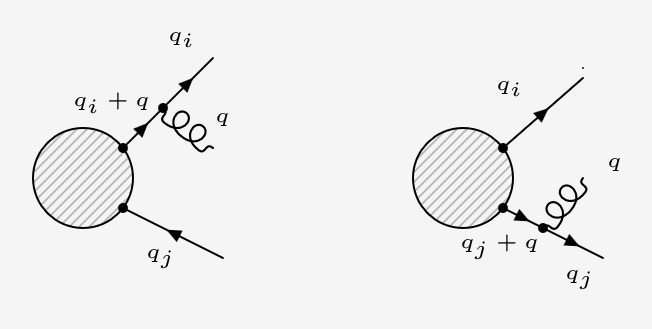
\includegraphics[width=0.85\textwidth]{images/QQ/qqg-diagrams.png}
\end{figure}
First we are going to consider a daughter quark from the splitting of a parent quark into a
quark and a gluon with an arbitrary spectator like an anti-quark, see the left picture above. where $ q_j+q $ is the momentum of the quark before splitting, $q$ the momentum of the gluon and $q_j$ of daughter quark respectively. The momentum of the spectator is $ q_j $. The distinction between daughter and parent vanishes, when the gluon becomes soft,  and a
singularity develops. The other possibility to get a singularity is surely if the gluon will be collinear to quark. The splitting functions are flavour independent since the strong interaction is flavour independent. Furthermore,
leading order splitting cannot change the flavour of a quark, thus we can write for the splitting functions In leading order QCD:
\begin{equation}
P_{{\bar{q_i}}{\bar{q_j}}}=P_{{q_i}{q_j}}=P_{{q}{q}} \delta_{ij}
\end{equation}
For this aim we have to take any diagram to the account which can have the same splitting. Since there is no distinction between quark and anti-quark, one can imagine exact the same splitting variation for anti-quark with a quark as a spectator, see the right picture above.


\pagebreak
\section{Matrix element of a quark with a gluon radiation $ |M_1|^2 $}

\begin{figure}[h!]
\centering
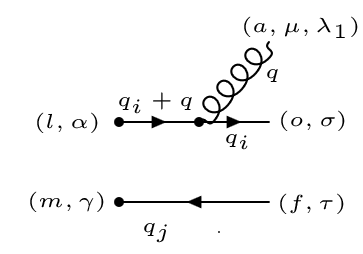
\includegraphics[scale=0.7]{images/QQ/qgqbarM.png}
\end{figure}
If one simply calculates the amplitude of this diagram, one gets:
\begin{equation}
M_1 = [{\bar{u}}_{\sigma}(q_i) (-ig_s \gamma^{\mu}\times {[T^a]_o}^l)  \frac{i(\not{q_i} + \not{q})}{(q_i + q)^2} {\varepsilon^{\lambda_1}}_{\mu} (q)]\: [{v}_{\tau}(q_j)]
\end{equation}
For the quadratic matrix element we need the dagger of $ M_1 $ as well.
\begin{figure}[h!]
\centering
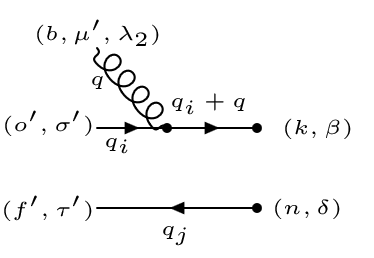
\includegraphics[scale=0.7]{images/QQ/qgqbarMDega.png}
\end{figure}

\begin{equation}
{M_1}^{\dagger} = [\frac{-i(\not{q_i} + \not{q})}{(q_i + q)^2} \:  (ig_s \gamma^{{\mu}^{\prime}}\times {[T^b]_{o\:^{\prime}}}^k) \: u_{{\sigma}^{\prime}}(q_i) \: {\varepsilon^{\lambda_2}}_{{\mu}^{\prime}} (q)][{\bar{v}}_{{\tau}^{\prime}}(q_j)]
\end{equation}
\pagebreak
\begin{figure}[h!]
\centering
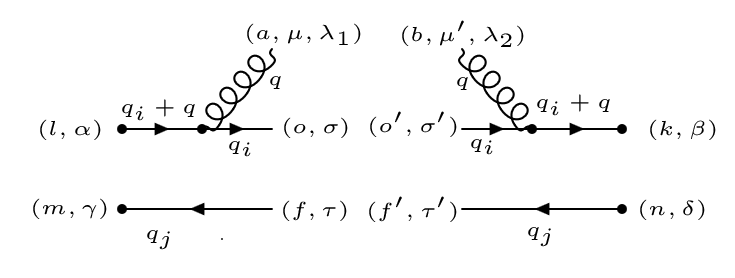
\includegraphics[width=0.85\textwidth]{images/QQ/qgqbarMSquer.png}
\end{figure}
After multiplying $ {M_1}^{\dagger} $ and $ {M_1} $ we get the desired result.
\begin{equation}
\begin{split}
|M_1|^2=M_1\:{\color[RGB]{255,0,0} {M_1}^{\dagger}} = [{\bar{u}}_{\sigma}(q_i)\: (-ig_s \gamma^{\mu}\times {[T^a]_o}^l) \: \frac{i(\not{q_i} + \not{q})}{(q_i + q)^2}\:\: {\varepsilon^{\lambda_1}}_{\mu} (q)] [{v}_{\tau}(q_j)]\: \\
\quad\quad\quad\quad\quad\quad\quad\quad\:\:{\color[RGB]{255,0,0}[\frac{-i(\not{q_i} + \not{q})}{(q_i + q)^2} \:  (ig_s \gamma^{{\mu}^{\prime}}\times {[T^b]_{o\:^{\prime}}}^k) \: u_{{\sigma}^{\prime}}(q_i) \: {{\varepsilon^{\lambda_2}}_{{\mu}^{\prime}}}^* (q)][{\bar{v}}_{{\tau}^{\prime}}(q_j)]}
\end{split}
\end{equation}
Now it's time to connect those terms which are related to each other.

\begin{equation}
\begin{split}
|M_1|^2=[\frac{-i(\not{q_i} + \not{q})}{(q_i + q)^2} \:
 \:  (ig_s \gamma^{{\mu}^{\prime}}\times {[T^b]_{o\:^{\prime}}}^k) \: {\bar{u}}_{\sigma}(q_i)\:u_{{\sigma}^{\prime}}(q_i) \: {{\varepsilon^{\lambda_2}}_{{\mu}^{\prime}}^* (q) {\varepsilon^{\lambda_1}}_{\mu} (q)} \\
\times (-ig_s \gamma^{\mu}\times {[T^a]_o}^l) \: \frac{i(\not{q_i} + \not{q})}{(q_i + q)^2} ]
[{\bar{v}}_{{\tau}^{\prime}}(q_j) {v}_{\tau}(q_j)]
\end{split}
\end{equation}

Sum over the lorenz index $({\sigma},{\sigma}^{\prime})$ and $({\tau},{\tau}^{\prime})$ and spin addition relation leads to:
 
\begin{equation}
\begin{split}
\displaystyle\sum\limits_{{\sigma},{\sigma}^{\prime}} {\bar{u}}_{\sigma}(q_i)\:u_{{\sigma}^{\prime}}(q_i) = \not{q_i} \delta^{{o}{o}^{\prime}},\\
\displaystyle\sum\limits_{{\tau},{\tau}^{\prime}} {\bar{v}}_{\tau}(q_j)\:v_{{\tau}^{\prime}}(q_j) = \not{q_j} \delta^{{f}{f}^{\prime}}
\end{split}
\end{equation}
Sum over polarization index $({\lambda_{1}},{\lambda}_{2})$ :
\begin{equation}
\begin{split}
 \displaystyle\sum\limits_{{\mu},{\mu}^{\prime}} {{\varepsilon^{\lambda_2}}_{{\mu}^{\prime}}^* (q) {\varepsilon^{\lambda_1}}_{\mu} (q)} = -g_{{\mu}{\mu}^{\prime}} \delta^{{a}{b}}
\end{split}
\end{equation}
The matrix element will be simplified with: 
\begin{equation}
\begin{split}
|M_1|^2=\frac{-g_s^2  {[T^a]_{o}}^k \: {[T^a]_o}^l }{(q_i + q)^2 (q_i + q)^2}
[(\not{q_i} + \not{q}) \:
 \:  \gamma^{{\mu}^{\prime}} \: \not{q_i} \: g_{{{\mu}^{\prime}}{\mu}} 
\gamma^{\mu} \: (\not{q_i} + q)]
[\not{q_j}]
\end{split}
\end{equation}

When we contract all related indices we will be actually able to make a statements about the last result.
\begin{equation}
\begin{split}
|M_1|^2=\frac{-g_s^2  {[T^a]_{o}}^k \: {[T^a]_o}^l }{(q_i + q)^2 (q_i + q)^2}
[(\not{q_i} + \not{q}) \:
 \:  \gamma^{{\mu}^{\prime}} \: \not{q_i} \: 
\gamma_{{\mu}^{\prime}} \: (\not{q_i} + q)]
[\not{q_j}]
\end{split}
\end{equation}

In other words we expect the tree level diagram from LO and a number:\\
\begin{figure}[h!]
\centering
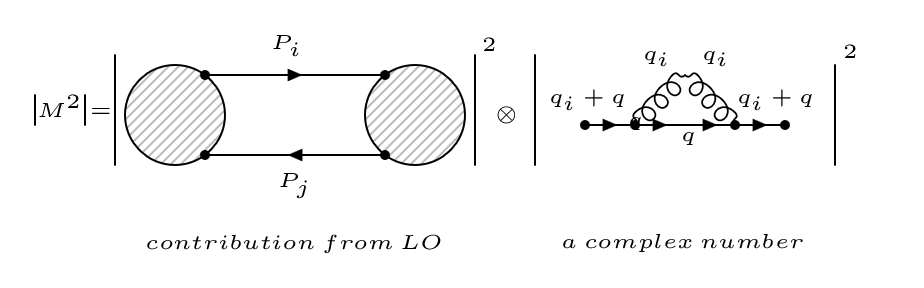
\includegraphics[width=0.85\textwidth]{images/QQ/expectationqg-qbar.png}
\end{figure}
Which graphically means:\\
\begin{equation}
\begin{split}
|M_1|^2=\frac{-g_s^2  {[T^a]_{o}}^k \: {[T^a]_o}^l }{(q_i + q)^2 (q_i + q)^2}
[\not{P_i}]
[\not{P_j}]\:\otimes \: {\color[RGB]{255,0,0} (a\: complex\: number)}
\end{split}
\end{equation}  
Let's calculate the contribution and compare the final result with this expectation:
\begin{equation}
\begin{split}
N=&: \gamma^{{\mu}^{\prime}} \not{q_i} \: \gamma_{{\mu}^{\prime}} = {q_{i\sigma}} \: \gamma^{{\mu}^{\prime}} \gamma^{\sigma} \:\: \gamma_{{\mu}^{\prime}}\\
=& \: {q_{i\sigma}} \: (\lbrace{\gamma^{{\mu}^{\prime}}}, {\gamma^{\sigma}}\rbrace \: - {\gamma^{\sigma}}{\gamma^{{\mu}^{\prime}}})\gamma_{{\mu}^{\prime}}\\
=& \:{q_{i\sigma}} \: 2g^{{{\mu}^{\prime}}{\sigma}} \: \gamma_{{\mu}^{\prime}} \: - \:d\:{\gamma^{\sigma}}\\
=& \:(2-d) \not{q_i}
\end{split}
\end{equation}
Simplification of the bracket:
\begin{equation}
\begin{split}
|M_1|^2=-(2-d)\:\frac{g_s^2  {[T^a]_{o}}^k \: {[T^a]_o}^l }{(q_i + q)^2 (q_i + q)^2}
[(\not{q_i} + \not{q}) \:
 \:\not{q_i} \: 
 \: (\not{q_i} + q)]
[\not{q_j}]
\end{split}
\end{equation}

\begin{equation}
\begin{split}
|M_1|^2=-(2-d)\:\frac{g_s^2  {[T^a]_{o}}^k \: {[T^a]_o}^l }{(q_i + q)^2 (q_i + q)^2}
[\not{q_i} \not{q_i} \not{q_i} \: + \: \not{q_i} \not{q_i} \not{q} \: + \: \not{q} \not{q_i} \not{q_i} \:+\: \not{q} \not{q_i} \not{q}]
[\not{q_j}]
\end{split}
\end{equation}

Momenta are on-shell, so:
\begin{equation}
\begin{split}
\not{q_i}\: \not{q_i} &= {q_i}^2= {m_i}^2\\
\not{q} \: \not{q} &= {q}^2= {m}^2\\
\not{q_j}\not{q_j} &= {q_j}^2= {m_j}^2
\end{split}
\end{equation}

we can first neglect the mass of patrons:

\begin{equation}
\begin{split}
|M_1|^2=-(2-d)\:\frac{g_s^2  {[T^a]_{o}}^k \: {[T^a]_o}^l }{(2q_i q)(2q_i q)}
[\not{q} \not{q_i} \not{q}]
[\not{q_j}]
\end{split}
\end{equation}
Here we need to make the terms in the brackets simpler and:
\begin{equation}
\begin{split}
L=& \not{q} \not{q_i} \not{q} =\not{q}[{q_{i\sigma}} q_{\mu} \: (\lbrace{\gamma^{\mu}}, {\gamma^{\sigma}}\rbrace - {\gamma^{\sigma}}{\gamma^{\mu}})]\\ 
=& \not{q}[2{q_{i}}^{\mu} q_{\mu} - {q_{i\sigma}}q_{\mu}{\gamma^{\mu}}{\gamma^{\sigma}}\\
=& \not{q} (2q_i q)-q_{\mu}{q_{i\sigma}}q_{\mu}[{\gamma^{\mu}}{\gamma^{\mu}}{\gamma^{\sigma}}]\\
=& \not{q} (2q_i q)-q_{\mu}{q_{i\sigma}}q_{\mu}[\frac{{\gamma^{\mu}}{\gamma^{\mu}}}{2} +\frac{{\gamma^{\mu}}{\gamma^{\mu}}}{2}]{\gamma^{\sigma}}\\
=& \not{q} (2q_i q)-q_{\mu}{q_{i\sigma}}q_{\mu}[g^{{\mu}{\mu}}]{\gamma^{\sigma}}\\
=& \not{q} (2q_i q)-q_{\mu}{q_{i\sigma}}q^{\mu}{\gamma^{\sigma}}
=\not{q} (2q_i q)-q^2 \not{q_i}\\
=& \not{q} (2q_i q)
\end{split}
\end{equation}
After inserting the last result of $ L $ and simplify the term $ (2q_i q) $ from the denominator and nominator, we get:
\begin{equation}
\begin{split}
|M_1|^2=-(2-d)\:\frac{g_s^2  {[T^a]_{o}}^k \: {[T^a]_o}^l }{2y(1-2z+2z^2)(p_i \cdot p_j)}
[\not{q}]
[\not{q_j}]
\end{split}
\end{equation}
Now we are going to use the parametrisation from equation (1) to reduce the 3-member matrix element to 2-member and take out the singularity term from the amplitude.
\begin{equation}
\begin{split}
|M_1|^2=(d-2)\:\frac{g_s^2  {[T^a]_{o}}^k \: {[T^a]_o}^l }{2y(1-2z+2z^2)(p_i \cdot p_j)}
[(1-z) \not{p_i}+zy \not{p_j} - \sqrt{zy(1-z)} \not{{m}_{\bot}}]
[(1-y) \not{p_j}]
\end{split}
\end{equation}
Multiplying the both sides 
\begin{equation}
\begin{split}
|M_1|^2=(d-2)\:\frac{g_s^2  {[T^a]_{o}}^k \: {[T^a]_o}^l }{2y(1-2z+2z^2)(p_i \cdot p_j)}
[(1-z)(1-y) \not{p_i}\not{p_j} \\
+zy(1-y) \not{p_j}\not{p_j} + (1-y)\sqrt{zy(1-z)} \not{{m}_{\bot}}\not{p_j}]
\end{split}
\end{equation}
Under consideration of the fact that $ p_i $ and $ p_j $ are the on-shell momenta of the emitter and spectator partons, we can ignore the terms with $ \not{p_i} \not{p_i} $ and $ \not{p_j} \not{p_j} $.
The $ {p_i} \cdot  {m}_{\bot} $ and $ {p_j} \cdot  {m}_{\bot} $ are always $ 0 $ because the $ p_i $ and $ p_j $ are lightlike, i.e. zero transverse component. So those terms can be neglected.


\begin{equation}
\begin{split}
|M_1|^2=\frac{g_s^2  {[T^a]_{o}}^k \: {[T^a]_o}^l }{(p_i \cdot p_j)}
[\not{p_i}][\not{p_j}]\otimes\frac{(d-2)(1-z)(1-y)}{2y(1-2z+2z^2)}
\end{split}
\end{equation}

As discussed, we get a contribution from the LO a complex number. As you can see, the number is just for $ y \rightarrow 0 $ singular and not for $ z \rightarrow 1 $.

\newpage

\section{Matrix element of an anti-quark with a gluon radiation $ |M_2|^2 $}

%\begin{figure}[h!]
%\centering
%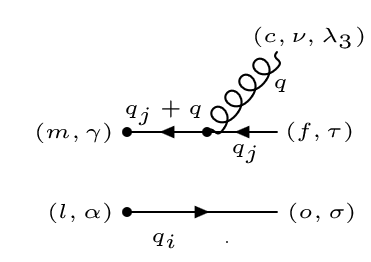
\includegraphics[scale=0.7]{images/QQ/qbargqM.png}
%\end{figure}
%
%\begin{equation}
%M_2 = [\frac{i(\not{q_j} + \not{q})}{(q_j + q)^2} (-ig_s \gamma^{\nu}\times {[T^c]_f}^m) \:{v}_{\tau}(q_j)\: {\varepsilon^{\lambda_3}}_{\nu} (q)]\: [{u}_{\sigma}(q_i)]
%\end{equation}
%\begin{figure}[h!]
%\centering
%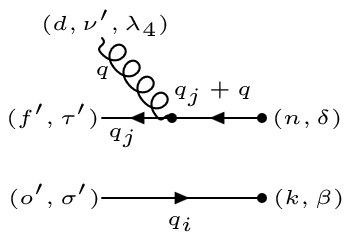
\includegraphics[scale=0.7]{images/QQ/qbargqMDega.png}
%\end{figure}
%\begin{equation}
%M_2^{\dagger} = [\bar{v}_{{\tau}^{\prime}}(q_j) \: (ig_s \gamma^{{\nu}^{\prime}}\times {[T^d]_{f^{\prime}}}^n) \: \frac{-i(\not{q_j} + \not{q})}{(q_j + q)^2} \: {\varepsilon^{\lambda_4}}_{{\nu}^{\prime}} (q)]\: [\bar{u}_{{\sigma}^{\prime}}(q_i)]
%\end{equation}
the same procedure is used to obtain the matrix element for an anti-quark with a single gluon emission.
\begin{figure}[h!]
\centering
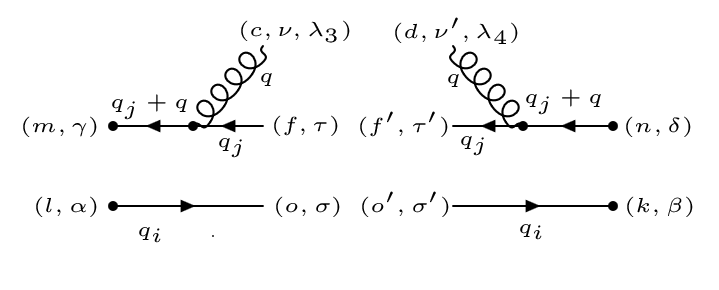
\includegraphics[width=0.85\textwidth]{images/QQ/qbargqMSquer.png}
\end{figure}

\begin{equation}
\begin{split}
|M_2|^2=M_2\:{\color[RGB]{255,0,0} {M_2}^{\dagger}} = [\frac{i(\not{q_j} + \not{q})}{(q_j + q)^2} (-ig_s \gamma^{\nu}\times {[T^c]_f}^m) \:{v}_{\tau}(q_j)\: {\varepsilon^{\lambda_3}}_{\nu} (q)]\: [{u}_{\sigma}(q_i)]\: \\
\quad\quad\quad\quad\quad\quad\quad\quad\:\:{\color[RGB]{255,0,0}[\bar{v}_{{\tau}^{\prime}}(q_j) \: (ig_s \gamma^{{\nu}^{\prime}}\times {[T^d]_{f^{\prime}}}^n) \: \frac{-i(\not{q_j} + \not{q})}{(q_j + q)^2} \: {\varepsilon^{\lambda_4}}_{{\nu}^{\prime}} (q)]\: [\bar{u}_{{\sigma}^{\prime}}(q_i)]}
\end{split}
\end{equation}


\begin{equation}
\begin{split}
|M_2|^2 =\frac{g_s^2 \: {[T^c]_f}^m \: {[T^d]_{f^{\prime}}}^n }{(q_j + q)^2 (q_j + q)^2} [(\not{q_j} + \not{q}) \gamma^{\nu}  \:{v}_{\tau}(q_j)\bar{v}_{{\tau}^{\prime}}(q_j)\: {\varepsilon^{\lambda_3}}_{\nu} (q){\varepsilon^{\lambda_4}}_{{\nu}^{\prime}}  (q) \gamma^{{\nu}^{\prime}}(\not{q_j} + \not{q})]\: \\
[{u}_{\sigma}(q_i) ]
\: [\bar{u}_{{\sigma}^{\prime}}(q_i)]
\end{split}
\end{equation}

and after sum over the lorenz and polarization indexes like $({\sigma},{\sigma}^{\prime})$, $({\tau},{\tau}^{\prime})$ and $({\lambda_{3}},{\lambda}_{4})$ as well and using the spin addition relation:
 
%\begin{equation}
%\begin{split}
%\displaystyle\sum\limits_{{\sigma},{\sigma}^{\prime}} {\bar{u}}_{\sigma}(q_i)\:u_{{\sigma}^{\prime}}(q_i) = \not{q_i} \delta^{{o}{o}^{\prime}},\\
%\displaystyle\sum\limits_{{\tau},{\tau}^{\prime}} {\bar{v}}_{\tau}(q_j)\:v_{{\tau}^{\prime}}(q_j) = \not{q_j} \delta^{{f}{f}^{\prime}}
%\end{split}
%\end{equation}
%
%\begin{equation}
%\begin{split}
% \displaystyle\sum\limits_{{\nu},{\nu}^{\prime}} {{\varepsilon^{\lambda_4}}_{{\nu}^{\prime}}^* (q) {\varepsilon^{\lambda_3}}_{\nu} (q)} = -g_{{\nu}{\nu}^{\prime}} \delta^{{c}{d}}
%\end{split}
%\end{equation}

\begin{equation}
\begin{split}
|M_2|^2 =\frac{g_s^2 \: {[T^c]_f}^m \: {[T^c]_{f}}^n }{(q_j + q)^2 (q_j + q)^2} [(\not{q_j} + \not{q}) \gamma^{\nu}  \:\not{q_j}\: (-g_{{\nu}{{\nu}^{\prime}}}) \gamma^{{\nu}^{\prime}}(\not{q_j} + \not{q})]\: 
[\not{q_i} ]
\end{split}
\end{equation}

Analogous to the last calculation from the previous section:

\begin{equation}
\begin{split}
|M_2|^2 =(d-2) \frac{g_s^2 \: {[T^c]_f}^m \: {[T^c]_{f}}^n }{(2qq_j)} [\not{q}]\: 
[\not{q_i} ]
\end{split}
\end{equation}
finally, we achieve:
\begin{equation}
\begin{split}
|M_2|^2=\frac{g_s^2 \: {[T^c]_f}^m \: {[T^c]_{f}}^n }{(p_i \cdot p_j)}
[\not{p_i}][\not{p_j}]\otimes \frac{-(d-2)yz^2}{2(1-z)(1-y)}
\end{split}
\end{equation}
Interestingly, here is a term with $y$ concerning the gluon radiation from an anti-quark. This means that this result cannot contribute to the collinear limit for soft gluon $ y \rightarrow 0 $.
\newpage

\section{Interference contribution}
So far most of the work is done and we just have to put the results of $M_1$ and ${M_2}^{\dagger}$ next to each other, as we can see in the diagram. So we still get the interference contribution. 
\begin{figure}[h!]
\centering
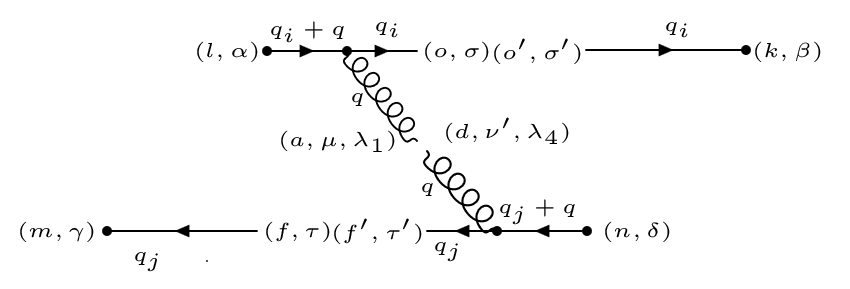
\includegraphics[width=0.85\textwidth]{images/QQ/M1M2Degaqqg.png}
\end{figure}
Using the results from the previous section and we received:
\begin{equation}
\begin{split}
M_1\:{\color[RGB]{255,0,0} {M_2}^{\dagger}} = [{\bar{u}}_{\sigma}(q_i)\: (-ig_s \gamma^{\mu}\times {[T^a]_o}^l) \: \frac{i(\not{q_i} + \not{q})}{(q_i + q)^2}\:\: {\varepsilon^{\lambda_1}}_{\mu} (q)] [{v}_{\tau}(q_j)]\: \\
\quad\quad\quad\quad\quad\quad\quad\quad\:\:{\color[RGB]{255,0,0}[\bar{v}_{{\tau}^{\prime}}(q_j) \: (ig_s \gamma^{{\nu}^{\prime}}\times {[T^d]_{f^{\prime}}}^n) \: \frac{-i(\not{q_j} + \not{q})}{(q_j + q)^2} \: {\varepsilon^{\lambda_4}}_{{\nu}^{\prime}} (q)]\: [{u}_{{\sigma}^{\prime}}(q_i)]}
\end{split}
\end{equation}

%Kommentar

\begin{equation}
\begin{split}
M_1\: {M_2}^{\dagger} = \frac{g_s^2 {[T^a]_o}^l \:{[T^d]_{f^{\prime}}}^n }{(2q_i q)(2q_j q)} [\not{q_i}\: \gamma^{\mu} \: (\not{q_i} + \not{q})\: ]{\varepsilon^{\lambda_1}}_{\mu} (q) \: {\varepsilon^{\lambda_4}}_{{\nu}^{\prime}} (q) \\
\:[\not{q_j} \:\gamma^{{\nu}^{\prime}} \: (\not{q_j} + \not{q})]\:
\end{split}
\end{equation}

\begin{equation}
\begin{split}
M_1\: {M_2}^{\dagger} = \frac{g_s^2 {[T^a]_o}^l \:{[T^a]_{f^{\prime}}}^n }{(2q_i q)(2q_j q)} [\not{q_i}\: \gamma^{\mu} \: (\not{q_i} + \not{q})\: ] -g_{{\mu}{{\nu}^{\prime}}} \\
\:[\not{q_j} \:\gamma^{{\nu}^{\prime}} \: (\not{q_j} + \not{q})]\:
\end{split}
\end{equation}



\begin{equation}
\begin{split}
M_1\: {M_2}^{\dagger} = \frac{-g_s^2 {[T^a]_o}^l \:{[T^a]_{f^{\prime}}}^n }{(2q_i q)(2q_j q)} [\not{q_i}\: \gamma^{\mu} \: (\not{q_i} + \not{q})\: ]
\:[\not{q_j} \:\gamma_{\mu} \: (\not{q_j} + \not{q})]\:
\end{split}
\end{equation}

%Kommentar 

Expectation:
\begin{figure}[h!]
\centering
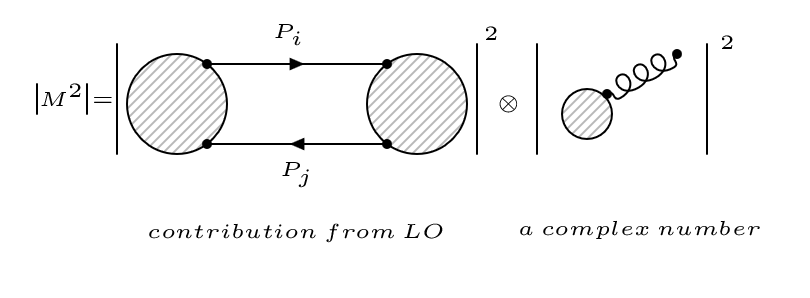
\includegraphics[width=0.85\textwidth]{images/QQ/expectationM1M2dagger.png}
\end{figure}

%Kommentar

\begin{equation}
\begin{split}
M_1\: {M_2}^{\dagger} = \frac{-g_s^2 {[T^a]_o}^l \:{[T^a]_{f^{\prime}}}^n }{(2q_i q)(2q_j q)} [(\not{q_i} + \not{q})\: \gamma^{\mu} \:  \not{q_i}\:]
\:[(\not{q_j} + \not{q}) \:\gamma_{\mu} \:\not{q_j} ]\:
\end{split}
\end{equation}

%Kommentra

\begin{align}
\begin{split}
&M_1\: {M_2}^{\dagger} = \frac{-g_s^2 {[T^a]_o}^l \:{[T^a]_{f^{\prime}}}^n }{(2q_i q)(2q_j q)} [-(\not{q_i} + \not{q})\:\not{q_i}\: \gamma^{\mu} \:+2(\not{q_i} + \not{q})\:{q_{i}}^{\mu}]\:\:\:\:\:\:\:\:\:\:\:\:\:\:\:\:\:\:\:\:\:\:\:\:\:\:\:\:\:\:\:\:\:\:\:\:\:\:\:\:\:\:\\
&\:[-(\not{q_j} + \not{q}) \not{q_j} \:\gamma_{\mu} \: + 2(\not{q_j} + \not{q}) {q_{j{\mu}}}]\: \\
\Rightarrow
&M_1\: {M_2}^{\dagger} = \frac{-g_s^2 {[T^a]_o}^l \:{[T^a]_{f^{\prime}}}^n }{(2q_i q)(2q_j q)} 
[(\not{q_i} + \not{q})\:\not{q_i}\: \gamma^{\mu}] \:[(\not{q_j} + \not{q}) \not{q_j} \gamma_{\mu}] \\
&-2[(\not{q_i} + \not{q})\:\not{q_i}\: \gamma^{\mu}]\:[ (\not{q_j} + \not{q}) {q_{j{\mu}}}]
\:-2[(\not{q_i} + \not{q})\:{q_{i}}^{\mu}][(\not{q_j} + \not{q}) \not{q_j} \:\gamma_{\mu}]\\
&+4[(\not{q_i} + \not{q})\:{q_{i}}^{\mu}][(\not{q_j} + \not{q}) {q_{j{\mu}}}]
\end{split}
\end{align}
The middle terms disappear due to the influence of the gamma matrices if the sequence of the matrices is reversed, so that the two terms become the same, because $ AB = -BA $:

%Kommentar

\begin{equation}
\begin{split}
&M_1\: {M_2}^{\dagger} = \frac{-g_s^2 {[T^a]_o}^l \:{[T^a]_{f^{\prime}}}^n }{(2q_i q)(2q_j q)} 
[(\not{q_i} + \not{q})\:\not{q_i}\: \gamma^{\mu}] \:[(\not{q_j} + \not{q}) \not{q_j} \gamma_{\mu}] \\
&-2[(\not{q_i} + \not{q})\:\not{q_i}\:\not{q_{j}} ]\:[ \not{q_j} + \not{q} ]
\:-2[\not{q_i} + \not{q}\:][(\not{q_j} + \not{q}) \not{q_j} \:\not{q_i}]\\
&+4[(\not{q_i} + \not{q})\:{q_{i}}^{\mu}][(\not{q_j} + \not{q}) {q_{j{\mu}}}]
\end{split}
\end{equation}

%Kommentar

\begin{align}
\begin{split}
&M_1\: {M_2}^{\dagger} = \frac{-g_s^2 {[T^a]_o}^l \:{[T^a]_{f^{\prime}}}^n }{(2q_i q)(2q_j q)} 
[(\not{q_i} + \not{q})\:\not{q_i}\: \gamma^{\mu}] \:[(\not{q_j} + \not{q}) \not{q_j} \gamma_{\mu}]\:\:\:\:\:\:\:\:\:\:\:\:\:\:\:\:\:\:\:\:\:\: \\
&+4[(\not{q_i} + \not{q})\:{q_{i}}^{\mu}][(\not{q_j} + \not{q}) {q_{j{\mu}}}]
\end{split}
\end{align}
Now we use the old parametrization to collect the singularities.
%\begin{equation}
%\begin{split}
%&M_1\: {M_2}^{\dagger} = \frac{-g_s^2 \:\:{[T^a]_o}^l \:{[T^a]_{f^{\prime}}}^n }{4(1-z)(1-y)y(1-2z+2z^2)(p_i \cdot p_j)(p_i \cdot p_j)} \\
%&[y(1-2z+2z^2)\not{p_i}\:\not{p_j}\: \gamma^{\mu}] \:[(1-z)(1-y)\not{p_i} \not{p_j} \gamma_{\mu}] \\
%&+4({q_{i}}^{\mu} \cdot {q_{j{\mu}}})[(\not{q_i} + \not{q})][(\not{q_j} + \not{q})]
%\end{split}
%\end{equation}

\begin{align}
\begin{split}
&M_1\: {M_2}^{\dagger} = \frac{-g_s^2 \:\:{[T^a]_o}^l \:{[T^a]_{f^{\prime}}}^n }{4(1-z)(1-y)y(1-2z+2z^2)(p_i \cdot p_j)(p_i \cdot p_j)} \\
&[y(1-2z+2z^2)\not{p_i}\:\not{p_j}\: \gamma^{\mu}] \:[(1-z)(1-y)\not{p_i} \not{p_j} \gamma_{\mu}] \\
&+4(p_i \cdot p_j)[(\not{p_i} + y\not{p_j})][(1-z)\not{p_i} + (1+yz-y) \not{p_j} - \sqrt{zy(1-z)}\not{m}]
\end{split}
\end{align}
Here we can use the singular term in the denominator $ y(1-z) $ to drop the term with the same pre-factor and thus obtain:

\begin{align}
\begin{split}
&M_1\: {M_2}^{\dagger} = \frac{-g_s^2 \:\:{[T^a]_o}^l \:{[T^a]_{f^{\prime}}}^n }{y(1-2z+2z^2)(p_i \cdot p_j)} 
[\not{p_i}][\not{p_j}]\otimes\frac{z}{1-z}\:\:\:\:\:\:\:\:\:\:\:\:\:
\end{split}
\end{align}

\pagebreak

\section{Final result}
One could assume that for a complete result the contribution $ {M_1}^{\dagger} M_2 $ is still missing.
\begin{equation}
\lvert\:M\lvert^2\: = \lvert\:M_1\lvert^2\:+\lvert\:M_2\lvert^2\:+ M_1\: {M_2}^{\dagger} +{M_1}^{\dagger} M_2
\end{equation}
\begin{figure}[h!]
\centering
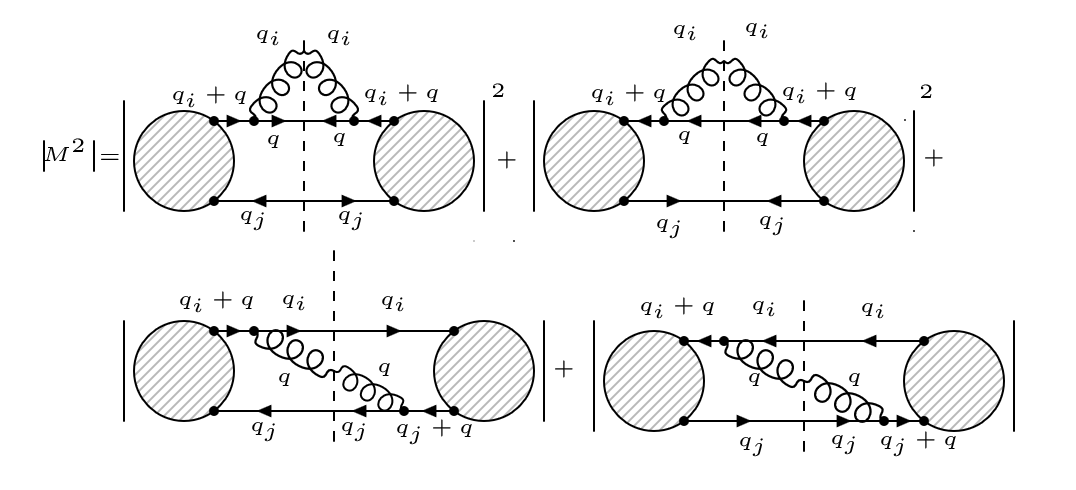
\includegraphics[width=0.85\textwidth]{images/QQ/qqgMSquer.png}
\end{figure}
It should be noted that it is completely sufficient to calculate $M_1\: {M_2}^{\dagger}$, because we know it from the quadratic amount of the complex numbers, we can calculate double of real part of $2RE(M_1\: {M_2}^{\dagger})$ instead of $ M_1\: {M_2}^{\dagger} +{M_1}^{\dagger} M_2 $ and that is exactly what is preferred here.
\begin{equation}
\lvert\:M\lvert^2\: = \lvert\:M_1\lvert^2\:+\lvert\:M_2\lvert^2\:+ {\color[RGB]{255,0,0} 2RE(M_1\: {M_2}^{\dagger})}
\end{equation}
\begin{figure}[h!]
\centering
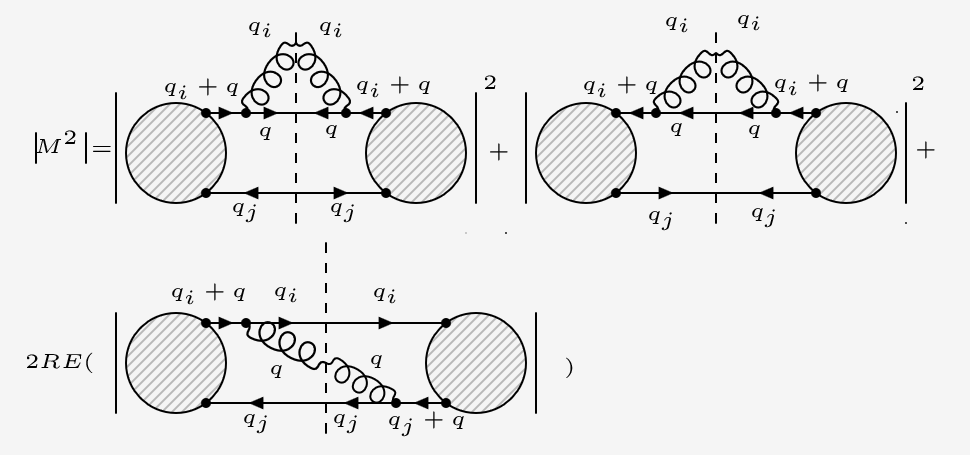
\includegraphics[width=0.85\textwidth]{images/QQ/REqqgMSquer.png}
\end{figure}
Let's just add up the results from the previous sections and get:
\begin{equation}
\begin{split}
&\lvert\:M\lvert^2\: = (d-2)(1-z)(1-y)\:\frac{g_s^2  {[T^a]_{o}}^k \: {[T^a]_o}^l }{2y(1-2z+2z^2)(p_i \cdot p_j)}
[\not{p_i}][\not{p_j}]\\
&-(d-2)yz^2\:\frac{g_s^2 \: {[T^c]_f}^m \: {[T^c]_{f}}^n }{2(1-z)(1-y)(p_i \cdot p_j)}
[\not{p_i}][\not{p_j}]\\
&+2RE((\frac{-2z}{z-1}) \frac{g_s^2 \:\:{[T^a]_o}^l \:{[T^a]_{f}}^n }{2y(1-2z+2z^2)(p_i \cdot p_j)} 
[\not{p_i}][\not{p_j}])
\end{split}
\end{equation}
Now we use the knowledge from the introduction about the calculation of the Colour factor. With Fritz equation:
\begin{equation}
{T^a}_{o\:k} \: {T^a}_{l\:o} = \frac{1}{2}(\delta_{oo}\delta_{lk}-\frac{1}{N}\delta_{ok}\delta_{lo})= \frac{1}{2}(N\delta_{lk}-\frac{1}{N}\delta_{lk})=C_F \delta_{lk}
\end{equation}
After summation over the final colour states and averaging over initial colour states we get:

\begin{equation}
{T^a}_{o\:k} \: {T^a}_{l\:o}=C_F \delta_{lk}=\frac{1}{N} \displaystyle\sum\limits_{l=1}^ N \delta_{lk}C_F=C_F
\end{equation}
The same calculation for $ {T^c}_{m\:f} \: {T^c}_{f\:n} $ and $ {T^a}_{o\:l} \: {T^a}_{f\:n} $ turns $ C_F $ out as the colour factor.
Now we are going to compute the splitting function in the case of the colinearity, wich means, if:
\begin{equation}
y \longrightarrow 0
\end{equation}

%\begin{equation}
%\begin{split}
%&\lvert\:M\lvert^2\: = (d-2)(1-z)(1-y)\:\frac{g_s^2 C_F}{2y(1-2z+2z^2)(p_i \cdot p_j)}
%[\not{p_i}][\not{p_j}]\\
%&-(d-2)yz^2\:\frac{g_s^2 \: C_F }{2(1-z)(1-y)(p_i \cdot p_j)}
%[\not{p_i}][\not{p_j}]\\
%&+2RE((\frac{-2z}{z-1}) \frac{g_s^2 C_F}{2y(1-2z+2z^2)(p_i \cdot p_j)} 
%[\not{p_i}][\not{p_j}]
%\end{split}
%\end{equation}

\begin{equation}
\lvert\:M\lvert^2\: = \frac{g_s^2 C_F}{2y(1-2z+2z^2)(p_i \cdot p_j)}[\not{p_i}][\not{p_j}] \otimes((d-2)(1-z)-\frac{4z}{z-1})\:
\end{equation}
\\
for $ d=4-2\epsilon $

%\begin{equation}
%\begin{split}
%\lvert\:M\lvert^2\: = C_F((4-2\epsilon-2)(1-z)+\frac{4z}{1-z})\:\frac{g_s^2}{2y(1-2z+2z^2)(p_i \cdot p_j)}[\not{p_i}][\not{p_j}]\\
%=C_F(\frac{2(1-\epsilon)(1-z)^2+4z}{1-z})\:\frac{g_s^2}{2y(1-2z+2z^2)(p_i \cdot p_j)}[\not{p_i}][\not{p_j}]\\
%C_F(\frac{2-4z+2z^2-\epsilon(1-z)^2+4z}{1-z})\:\frac{g_s^2}{2y(1-2z+2z^2)(p_i \cdot p_j)}[\not{p_i}][\not{p_j}]\\
%=C_F(\frac{(1+z^2)}{1-z}-\epsilon(1-z))\:\frac{g_s^2}{y(1-2z+2z^2)(p_i \cdot p_j)}[\not{p_i}][\not{p_j}]\\
%=\langle\:\hat{P_{qq}}\rangle\:\frac{g_s^2}{q_i \cdot q}[\not{p_i}][\not{p_j}]\\
%\end{split}
%\end{equation}

\begin{equation}
\begin{split}
\lvert\:M\lvert^2\: &=\frac{g_s^2}{y(1-2z+2z^2)(p_i \cdot p_j)}[\not{p_i}][\not{p_j}]\otimes C_F(\frac{(1+z^2)}{1-z}-\epsilon(1-z))\\
&=\frac{g_s^2}{q_i \cdot q}[\not{p_i}][\not{p_j}]\otimes \langle\:\hat{P_{qq}}\rangle\:\\
\end{split}
\end{equation}

With Alterali-Parisi splitting function $ \langle\:\hat{P_{qq}}\rangle\: $ in the collinear limes, which was mentioned in the previous chapter. This is exactly the confirmation of our calculation that our calculation was actually performed correctly, otherwise we would not have received the same splitting function for soft gluons.
\newpage

\section{Double-check the results with the new kinematic}
One could do exactly the same calculation for the new kinematics to see if you get the same result in the collinear limit. From the next chapter we will explicitly work with the new parametrisation, because we found that the old kinematics only work in NLO and one-single emission. 
\subsection*{$ |M_1|^2 $}

\begin{equation}
\begin{split}
|M_1|^2=(d-2)\:\frac{g_s^2  C_F }{(2k_1\cdot q_i)}
[\not{k_1} ][\not{q_k}]
\end{split}
\end{equation}

\begin{equation}
\begin{split}
&|M_1|^2=(d-2)\:\frac{g_s^2 \: C_F }{2y\: p_i \cdot Q}
[(\alpha_1 -y\beta_1(\frac{Q^2}{2p_i \cdot Q})) \not{p_i} + y\beta_1\not{Q} + \sqrt{y\alpha_1\beta_1}\not{n}_{\bot,1} ]\\
&[A_1\not{p_i} + A_2\not{Q} + \sqrt{1-y}\not{p_k}]
\end{split}
\end{equation}

\begin{equation}
\begin{split}
&|M_1|^2=(d-2)\:\frac{g_s^2 \: C_F }{2y\: p_i \cdot Q}
[(A_2(\alpha_1 -y\beta_1(\frac{Q^2}{2p_i \cdot Q}))+ A_1y\beta_1) {p_i}\cdot Q\\
&+(\alpha_1 -y\beta_1(\frac{Q^2}{2p_i \cdot Q}))\sqrt{1-y}p_i\cdot p_k+A_2 y\beta_1 Q^2+ \sqrt{1-y}\sqrt{y\alpha_1\beta_1}{n}_{\bot,1}\cdot p_k ]\\
\end{split}
\end{equation}

For the collinearity $ y \rightarrow 0 $ we'll get:

\begin{equation}
\begin{split}
&|M_1|^2=(d-2)\:\frac{g_s^2 \: C_F }{2y\: p_i \cdot Q}
[(A_2(\alpha_1 -y\beta_1(\frac{Q^2}{2p_i \cdot Q}))+ A_1y\beta_1) \not{p_i} \not{Q}\\
&+(\alpha_1 -y\beta_1(\frac{Q^2}{2p_i \cdot Q}))\sqrt{1-y}\not{p_i} \not{p_k}+A_2 y\beta_1 Q^2+ \sqrt{1-y}\sqrt{y\alpha_1\beta_1}\not{n}_{\bot,1} \not{p_k} ]\\
\end{split}
\end{equation}

\begin{equation}
\begin{split}
&|M_1|^2=(d-2)(1-\beta_1)\sqrt{1-y}\:\frac{g_s^2 \: C_F }{2y\: p_i \cdot Q}
[\not{p_i} \not{p_k} ]\\
\end{split}
\end{equation}

\subsection*{$ |M_2|^2 $}

\begin{equation}
\begin{split}
|M_2|^2 =(d-2) \frac{g_s^2 \: C_F }{2k_1 \cdot q_k} [\not{k_1}]\: 
[\not{q_i} ]
\end{split}
\end{equation}

\begin{equation}
\begin{split}
&|M_2|^2 =(d-2) \frac{g_s^2 \: C_F}{2k_1 \cdot q_k} [(\alpha_1 -y\beta_1(\frac{Q^2}{2p_i \cdot Q})) \not{p_i} + y\beta_1\not{Q} + \sqrt{y\alpha_1\beta_1}\not{n}_{\bot,1}]\: \\
&[(\beta_1 -\alpha_1 y(\frac{Q^2}{2p_i \cdot Q}))\not{p_i} + y\alpha_1\not{Q} - \sqrt{y\alpha_1\beta_1}\not{n}_{\bot,l} ]
\end{split}
\end{equation}

Which means:
\begin{equation}
\begin{split}
&|M_2|^2 \sim(d-2) \frac{g_s^2 \: C_F}{2k_1 \cdot q_k} y[...]\\
&\:\:\:\:\:\:\:\:|M_2|^2\rightarrow 0 \:\:\:\:\:\:\:\text{for}\:\:\:\:\: y\rightarrow 0
\end{split}
\end{equation}

\subsection*{$ M_1\: {M_2}^{\dagger} $}


\begin{equation}
\begin{split}
&M_1\: {M_2}^{\dagger} = \frac{-g_s^2\: C_F }{4y(1-\beta_1) (1-y)\:(p_i \cdot p_k)(p_i \cdot Q)} \\
&4(\beta_1 \sqrt{1-y}{p_i}\cdot {{p_k}})[\beta_1 \sqrt{1-y}\not{p_i} \not{p_k}+ (1-\beta_1) \sqrt{1-y}\not{p_i}\not{p_k}]
\end{split}
\end{equation}

\begin{equation}
\begin{split}
&M_1\: {M_2}^{\dagger} = \frac{-g_s^2\: C_F }{y(1-\beta_1) \:(p_i \cdot p_k)(p_i \cdot Q)} \beta_1( {p_i}\cdot {{p_k}})[\beta_1 \not{p_i} \not{p_k}+ (1-\beta_1) \not{p_i}\not{p_k}]
\end{split}
\end{equation}

\begin{equation}
\begin{split}
&M_1\: {M_2}^{\dagger} = \frac{\beta_1}{(1-\beta_1)}\: \frac{-g_s^2\: C_F }{y \:(p_i \cdot Q)} [\not{p_i} \not{p_k}]
\end{split}
\end{equation}
\newpage
\newpage
\chapter{Gluon gluon gluon emission kernel}

\begin{figure}[ht!]
\centering
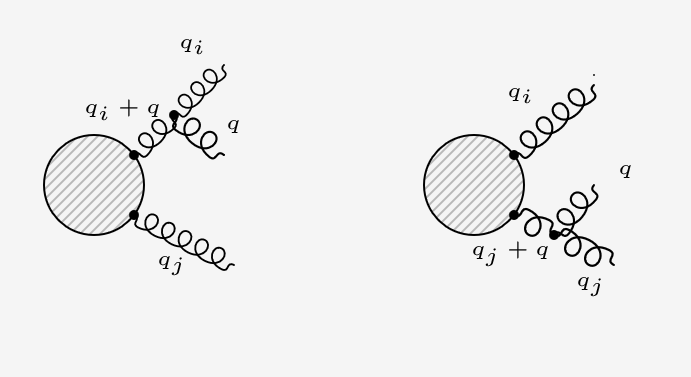
\includegraphics[width=0.85\textwidth]{images/GG/GGDiagrams.png}
\end{figure}
\pagebreak
\section{Gluon-Emitter Bubble}
\begin{figure}[ht!]
\centering
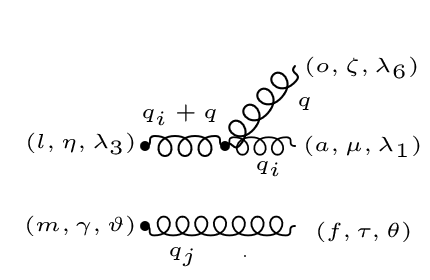
\includegraphics[scale=0.7]{images/GG/M1gg.png}
\end{figure}
\begin{equation}
\begin{split}
M_1=[\frac{-i}{(q +q_i)^2}(-g_s f^{\:a\:o\:l}(g^{{\mu}{\zeta}}(q -q_i)^{\eta}+g^{{\zeta}{\eta}}(-q-(q +q_i))^{\mu}+g^{{\eta}{\mu}}(q_i +q_i+q)^{\zeta})\\
{\varepsilon^{\lambda_1}}_{\mu} (q) {\varepsilon^{\lambda_6}}_{\zeta} (q)][{{\varepsilon^{\theta}}_{{\tau}^{\prime}}} (q_j)]
\end{split}
\end{equation}

\begin{equation}
\begin{split}
M_1=[\frac{-i}{(q_i +q)^2}(-g_s f^{\:a\:o\:l}(g^{{\mu}{\zeta}}(q-q_i)^{\eta}-g^{{\zeta}{\eta}}(2q +q_i)^{\mu}+g^{{\eta}{\mu}}(2q_i +q)^{\zeta})\\
{\varepsilon^{\lambda_1}}_{\mu} (q_i) {\varepsilon^{\lambda_6}}_{\zeta} (q)][{{\varepsilon^{\theta}}_{{\tau}^{\prime}}} (q_j)]
\end{split}
\end{equation}
\begin{figure}[ht!]
\centering
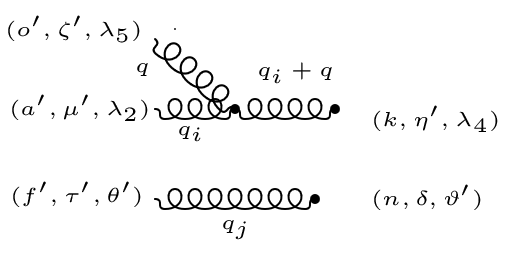
\includegraphics[scale=0.7]{images/GG/M1Daggergg.png}
\end{figure}
\begin{equation}
\begin{split}
{M_1}^{\dagger}=[\frac{i}{(q_i +q)^2}(-g_s f^{\:a^{\prime}\:k\: o^{\prime}}(-g^{{{\mu}^{\prime}}{{\eta}^{\prime}}}(2q_i+q)^{{\zeta}^{\prime}}+g^{{{\eta}^{\prime}}{{\zeta}^{\prime}}}(2q +q_i)^{{\mu}^{\prime}}+g^{{{\zeta}^{\prime}}{{\mu}^{\prime}}}(q_i-q)^{{\eta}^{\prime}})\\
{{\varepsilon^{\lambda_2}}_{{\mu}^{\prime}}}^* (q_i) {{\varepsilon^{\lambda_5}}_{{\zeta}^{\prime}}}^* (q)][{{\varepsilon^{{\theta}^{\prime}}}_{{\tau}^{\prime}}}^* (q_j)]
\end{split}
\end{equation}
\begin{figure}[ht!]
\centering
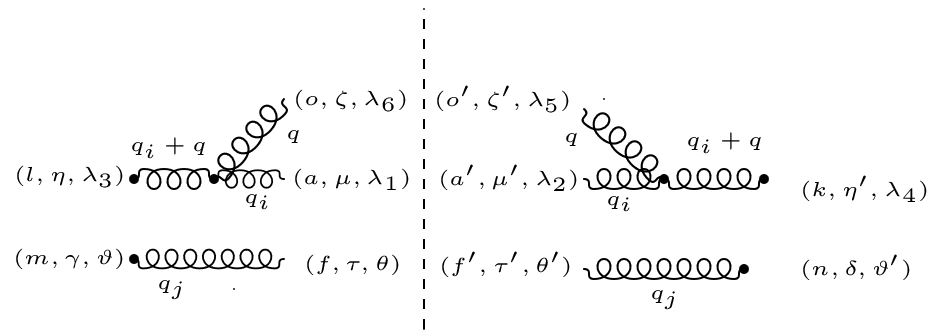
\includegraphics[width=0.95\textwidth]{images/GG/M1Squer.png}
\end{figure}
\begin{equation}
\begin{split}
|M_1|^2=[\frac{-i}{(q_i +q)^2}(-g_s f^{\:a\:o\:l}(g^{{\mu}{\zeta}}(q-q_i)^{\eta}-g^{{\zeta}{\eta}}(2q +q_i)^{\mu}+g^{{\eta}{\mu}}(2q_i +q)^{\zeta})\\
{\varepsilon^{\lambda_1}}_{\mu} (q_i)\:{{\varepsilon^{\lambda_2}}_{{\mu}^{\prime}}}^* (q_i) {\varepsilon^{\lambda_6}}_{\zeta} (q)\:{{\varepsilon^{\lambda_5}}_{{\zeta}^{\prime}}}^* (q)\\
(-g_s f^{\:a^{\prime}\:k\:o^{\prime}}(-g^{{{\mu}^{\prime}}{{\eta}^{\prime}}}(2q_i+q)^{{\zeta}^{\prime}}+g^{{{\eta}^{\prime}}{{\zeta}^{\prime}}}(2q +q_i)^{{\mu}^{\prime}}+g^{{{\zeta}^{\prime}}{{\mu}^{\prime}}}(q_i-q)^{{\eta}^{\prime}})\frac{i}{(q_i +q)^2}][g^{{\gamma}{\delta}}]
\end{split}
\end{equation}

\begin{equation}
\begin{split}
N\equiv g_{{\mu}{{\mu}^{\prime}}} g_{{\zeta}{{\zeta}^{\prime}}}[-g^{{\mu}{\zeta}}g^{{{\mu}^{\prime}}{{\eta}^{\prime}}}(q-q_i)^{{\eta}}(2q_i+q)^{{\zeta}^{\prime}}+g^{{\mu}{\zeta}}g^{{{\eta}^{\prime}}{{\zeta}^{\prime}}}(q-q_i)^{\eta}(2q +q_i)^{{\mu}^{\prime}}\\+g^{{\mu}{\zeta}}g^{{{\zeta}^{\prime}}{{\mu}^{\prime}}}(q-q_i)^{\eta}(q_i -q)^{{\eta}^{\prime}}+g^{{\zeta}{\eta}}g^{{{\mu}^{\prime}}{{\zeta}^{\prime}}}(2q +q_i)^{\mu}(2q_i+q)^{{\zeta}^{\prime}}\\
-g^{{\zeta}{\eta}}g^{{{\eta}^{\prime}}{{\zeta}^{\prime}}}(2q +q_i)^{\mu}(2q +q_i)^{{\mu}^{\prime}}-g^{{\zeta}{\eta}}g^{{{\zeta}^{\prime}}{{\mu}^{\prime}}}(2q +q_i)^{\mu}(q_i -q)^{{\eta}^{\prime}}\\
-g^{{\eta}{\mu}}g^{{{\mu}^{\prime}}{{\eta}^{\prime}}}(2q_i +q)^{\zeta}(2q_i+q)^{{\zeta}^{\prime}}+g^{{\eta}{\mu}}g^{{{\eta}^{\prime}}{{\zeta}^{\prime}}}(2q_i +q)^{\zeta}(2q +q_i)^{{\mu}^{\prime}}\\
+g^{{\eta}{\mu}}g^{{{\zeta}^{\prime}}{{\mu}^{\prime}}}(2q_i +q)^{\zeta}(q_i -q)^{{\eta}^{\prime}}][g^{{\gamma}{\delta}}]
\end{split}
\end{equation}


\begin{equation}
\begin{split}
N\equiv [-(q-q_i)^{{\eta}}(2q_i+q)^{{\eta}^{\prime}}+(q-q_i)^{\eta}(2q +q_i)^{{\eta}^{\prime}}+d(q-q_i)^{\eta}(q_i -q)^{{\eta}^{\prime}}\\+(2q +q_i)^{{\eta}^{\prime}}(2q_i+q)^{{\eta}}
-g^{{\eta}{{\eta}^{\prime}}}(2q +q_i)^{\mu}(2q +q_i)_{{\mu}}-(2q +q_i)^{\eta}(q_i -q)^{{\eta}^{\prime}}\\
-g^{{\eta}{{\eta}^{\prime}}}(2q_i +q)^{\zeta}(2q_i+q)_{{\zeta}}+(2q_i +q)^{{\eta}^{\prime}}(2q +q_i)^{{\eta}}
+(2q_i +q)^{\eta}(q_i -q)^{{\eta}^{\prime}}][g^{{\gamma}{\delta}}]
\end{split}
\end{equation}

\begin{equation}
\begin{split}
N\equiv [-({q}^{{\eta}}{q}^{{\eta}^{\prime}}+2{q}^{{\eta}}{q_i}^{{\eta}^{\prime}}-{q_i}^{{\eta}}{q}^{{\eta}^{\prime}}-2{q_i}^{{\eta}}{q_i}^{{\eta}^{\prime}})
+(2{q}^{{\eta}}{q}^{{\eta}^{\prime}}+{q}^{{\eta}}{q_i}^{{\eta}^{\prime}}-2{q_i}^{{\eta}}{q}^{{\eta}^{\prime}}-{q_i}^{{\eta}}{q_i}^{{\eta}^{\prime}})\\+(d{q}^{{\eta}}{q_i}^{{\eta}^{\prime}}-d{q}^{{\eta}}{q}^{{\eta}^{\prime}}-d{q_i}^{{\eta}}{q_i}^{{\eta}^{\prime}}+d{q_i}^{{\eta}}{q}^{{\eta}^{\prime}})+(4{q}^{{\eta}^{\prime}}{q_i}^{{\eta}}+2{q}^{{\eta}^{\prime}}{q}^{{\eta}}+2{q_i}^{{\eta}^{\prime}}{q_i}^{{\eta}}+{q_i}^{{\eta}^{\prime}}{q}^{{\eta}})\\
-(-2{q}^{{\eta}}{q}^{{\eta}^{\prime}}+2{q}^{{\eta}}{q_i}^{{\eta}^{\prime}}-{q_i}^{{\eta}}{q}^{{\eta}^{\prime}}+{q_i}^{{\eta}}{q_i}^{{\eta}^{\prime}})+(2{q}^{{\eta}^{\prime}}{q}^{{\eta}}+{q}^{{\eta}^{\prime}}{q_i}^{{\eta}}+4{q_i}^{{\eta}^{\prime}}{q}^{{\eta}}+2{q_i}^{{\eta}^{\prime}}{q_i}^{{\eta}})\\+(-{q}^{{\eta}}{q}^{{\eta}^{\prime}}+{q}^{{\eta}}{q_i}^{{\eta}^{\prime}}-2{q_i}^{{\eta}}{q}^{{\eta}^{\prime}}+2{q_i}^{{\eta}}{q_i}^{{\eta}^{\prime}})
-g^{{\eta}{{\eta}^{\prime}}}(5{q}^2+5{q_i}^2+8qq_i)][g^{{\gamma}{\delta}}]
\end{split}
\end{equation}

\begin{equation}
\begin{split}
N\equiv [(6-d){q}^{{\eta}}{q}^{{\eta}^{\prime}}+(d+3){q}^{{\eta}}{q_i}^{{\eta}^{\prime}}+(d+3){q_i}^{{\eta}}{q}^{{\eta}^{\prime}}+(6-d){q_i}^{{\eta}}{q_i}^{{\eta}^{\prime}}\\
-g^{{\eta}{{\eta}^{\prime}}}(5{q}^2+5{q_i}^2+8qq_i)][g^{{\gamma}{\delta}}]
\end{split}
\end{equation}

\begin{equation}
\begin{split}
|M_1|^2=\frac{g_s^2 \:f^{\:a\:o\:l}\: f^{\:a\:k\:o}}{(q_i +q)^2 (q_i +q)^2} [(6-d){q}^{{\eta}}{q}^{{\eta}^{\prime}}+(d+3){q}^{{\eta}}{q_i}^{{\eta}^{\prime}}+(d+3){q_i}^{{\eta}}{q}^{{\eta}^{\prime}}+(6-d){q_i}^{{\eta}}{q_i}^{{\eta}^{\prime}}\\
-g^{{\eta}{{\eta}^{\prime}}}(5{q}^2+5{q_i}^2+8qq_i)][g^{{\gamma}{\delta}}]
\end{split}
\end{equation}


\pagebreak
\subsection{One-loop corrections to the gluon self-energy diagram(Gluon-Emitter Bubble)}
\begin{figure}[h!]
\centering
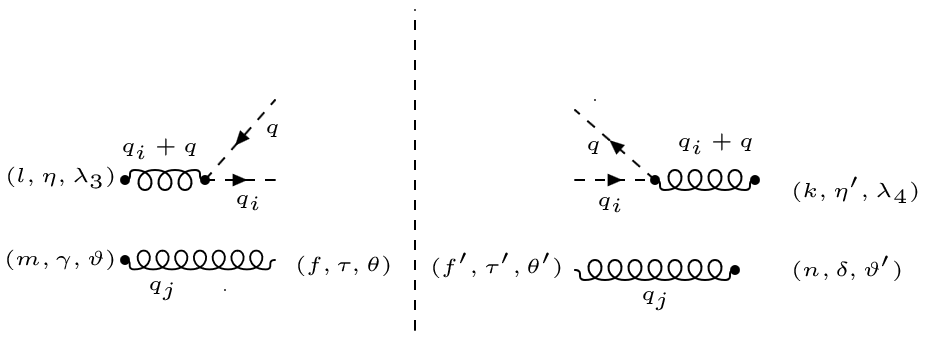
\includegraphics[width=0.95\textwidth]{images/GG/Ghost.png}
\end{figure}

\begin{equation}
\begin{split}
{{|M_1|}^2_{Ghost \:loop}}=\frac{g_s^2 \:f^{\:a\:o\:l}\: f^{\:a\:k\:o}}{(q_i +q)^2 (q_i +q)^2} [-{q_i}^{{\eta}}{q}^{{\eta}^{\prime}}-{q}^{{\eta}}{q_i}^{{\eta}^{\prime}}][g^{{\gamma}{\delta}}]
\end{split}
\end{equation}

\begin{equation}
\begin{split}
{|{M}^{\prime}_1|}^2 = {|M_1|}^2+{{|M_1|}^2_{Ghost \:loop}}\\=\frac{g_s^2 \:f^{\:a\:o\:l}\: f^{\:a\:k\:o}}{(q_i +q)^2 (q_i +q)^2}  [(6-d){q}^{{\eta}}{q}^{{\eta}^{\prime}}+(d+3){q}^{{\eta}}{q_i}^{{\eta}^{\prime}}\\+(d+3){q_i}^{{\eta}}{q}^{{\eta}^{\prime}}+(6-d){q_i}^{{\eta}}{q_i}^{{\eta}^{\prime}}-g^{{\eta}{{\eta}^{\prime}}}(5{q}^2+5{q_i}^2+8qq_i)-{q_i}^{{\eta}}{q}^{{\eta}^{\prime}}-{q}^{{\eta}}{q_i}^{{\eta}^{\prime}}][g^{{\gamma}{\delta}}]
\end{split}
\end{equation}

\begin{equation}
\begin{split}
{|{M}^{\prime}_1|}^2 =\frac{g_s^2 \:f^{\:a\:o\:l}\: f^{\:a\:k\:o}}{(q_i +q)^2 (q_i +q)^2}  [(6-d){q}^{{\eta}}{q}^{{\eta}^{\prime}}+(d+2){q}^{{\eta}}{q_i}^{{\eta}^{\prime}}\\+(d+2){q_i}^{{\eta}}{q}^{{\eta}^{\prime}}+(6-d){q_i}^{{\eta}}{q_i}^{{\eta}^{\prime}}-g^{{\eta}{{\eta}^{\prime}}}(8qq_i)][g^{{\gamma}{\delta}}]
\end{split}
\end{equation}

\begin{equation}
\begin{split}
{|{M}^{\prime}_1|}^2 =\frac{g_s^2 \:f^{\:a\:o\:l}\: f^{\:a\:k\:o}}{4y^2({\alpha_1}+\beta_1)^2\:(p_i\cdot Q) \:(p_i\cdot Q)} \\
[(6-d)(\zeta_1 {p_i}^{\eta} + \lambda_1{Q}^{\eta} + \sqrt{y\alpha_1\beta_1}{n^{\eta}}_{\bot,1})(\zeta_1 {p_i}^{{\eta}^{\prime}} + \lambda_1{Q}^{{\eta}^{\prime}} + \sqrt{y\alpha_1\beta_1}{n^{{\eta}^{\prime}}}_{\bot,1})\\
+(d+2)(\zeta_1 {p_i}^{\eta} + \lambda_1{Q}^{\eta} + \sqrt{y\alpha_1\beta_1}{n^{\eta}}_{\bot,1})(\zeta_q {p_i}^{{\eta}^{\prime}} + \lambda_q{Q}^{{\eta}^{\prime}} - \sqrt{y\alpha_1\beta_1}{n^{{\eta}^{\prime}}}_{\bot,1})\\
+(d+2)(\zeta_q {p_i}^{\eta} + \lambda_q{Q}^{\eta} - \sqrt{y\alpha_1\beta_1}{n^{\eta}}_{\bot,1})(\zeta_1 {p_i}^{{\eta}^{\prime}} + \lambda_1{Q}^{{\eta}^{\prime}} + \sqrt{y\alpha_1\beta_1}{n^{{\eta}^{\prime}}}_{\bot,1})\\
+(6-d)(\zeta_q {p_i}^{\eta} + \lambda_q{Q}^{\eta} - \sqrt{y\alpha_1\beta_1}{n^{\eta}}_{\bot,1})(\zeta_q {p_i}^{{\eta}^{\prime}} + \lambda_q{Q}^{{\eta}^{\prime}} - \sqrt{y\alpha_1\beta_1}{n^{{\eta}^{\prime}}}_{\bot,1})\\
-8g^{{\eta}{{\eta}^{\prime}}}[({\alpha_1}^2+{\beta_1}^2) p_i \cdot Q - ({\beta_1}(1-\beta_1)){n}_{\bot,1}\cdot{n}_{\bot,1}]][g^{{\gamma}{{\delta}}}]
\end{split}
\end{equation}

\begin{equation}
\begin{split}
{|{M}^{\prime}_1|}^2 =\frac{g_s^2 \:f^{\:a\:o\:l}\: f^{\:a\:k\:o}}{y^2\:(p_i\cdot Q) \:(p_i\cdot Q)} \\
[(6-d)[\zeta_1 \zeta_1 {p_i}^{\eta}{p_i}^{{\eta}^{\prime}}+\zeta_1 \lambda_1{p_i}^{\eta}{Q}^{{\eta}^{\prime}}+\zeta_1\sqrt{y\alpha_1\beta_1}{p_i}^{\eta}{n^{{\eta}^{\prime}}}_{\bot,1}\\
+\lambda_1\zeta_1 {Q}^{\eta}{p_i}^{{\eta}^{\prime}}+\lambda_1\lambda_1{Q}^{\eta}{Q}^{{\eta}^{\prime}}+\lambda_1\sqrt{y\alpha_1\beta_1}{Q}^{\eta}{n^{{\eta}^{\prime}}}_{\bot,1}\\
+\zeta_1\sqrt{y\alpha_1\beta_1} {n^{{\eta}}}_{\bot,1}{p_i}^{{\eta}^{\prime}}+\lambda_1\sqrt{y\alpha_1\beta_1}{n^{{\eta}}}_{\bot,1}{Q}^{{\eta}^{\prime}}+\sqrt{y\alpha_1\beta_1}\sqrt{y\alpha_1\beta_1}{n^{{\eta}}}_{\bot,1}{n^{{\eta}^{\prime}}}_{\bot,1}]\\
[(d+2)[\zeta_1 \zeta_q {p_i}^{\eta}{p_i}^{{\eta}^{\prime}}+\zeta_1 \lambda_q{p_i}^{\eta}{Q}^{{\eta}^{\prime}}-\zeta_1\sqrt{y\alpha_1\beta_1}{p_i}^{\eta}{n^{{\eta}^{\prime}}}_{\bot,1}\\
+\lambda_1\zeta_q {Q}^{\eta}{p_i}^{{\eta}^{\prime}}+\lambda_1\lambda_q{Q}^{\eta}{Q}^{{\eta}^{\prime}}-\lambda_1\sqrt{y\alpha_1\beta_1}{Q}^{\eta}{n^{{\eta}^{\prime}}}_{\bot,1}\\
+\zeta_q\sqrt{y\alpha_1\beta_1} {n^{{\eta}}}_{\bot,1}{p_i}^{{\eta}^{\prime}}+\lambda_q\sqrt{y\alpha_1\beta_1}{n^{{\eta}}}_{\bot,1}{Q}^{{\eta}^{\prime}}-\sqrt{y\alpha_1\beta_1}\sqrt{y\alpha_1\beta_1}{n^{{\eta}}}_{\bot,1}{n^{{\eta}^{\prime}}}_{\bot,1}]\\
[(d+2)[\zeta_q \zeta_1 {p_i}^{\eta}{p_i}^{{\eta}^{\prime}}+\zeta_q \lambda_1{p_i}^{\eta}{Q}^{{\eta}^{\prime}}+\zeta_q\sqrt{y\alpha_1\beta_1}{p_i}^{\eta}{n^{{\eta}^{\prime}}}_{\bot,1}\\
+\lambda_q\zeta_1 {Q}^{\eta}{p_i}^{{\eta}^{\prime}}+\lambda_q\lambda_1{Q}^{\eta}{Q}^{{\eta}^{\prime}}+\lambda_q\sqrt{y\alpha_1\beta_1}{Q}^{\eta}{n^{{\eta}^{\prime}}}_{\bot,1}\\
-\zeta_1\sqrt{y\alpha_1\beta_1} {n^{{\eta}}}_{\bot,1}{p_i}^{{\eta}^{\prime}}-\lambda_1\sqrt{y\alpha_1\beta_1}{n^{{\eta}}}_{\bot,1}{Q}^{{\eta}^{\prime}}-\sqrt{y\alpha_1\beta_1}\sqrt{y\alpha_1\beta_1}{n^{{\eta}}}_{\bot,1}{n^{{\eta}^{\prime}}}_{\bot,1}]\\
[(6-d)[\zeta_q \zeta_q {p_i}^{\eta}{p_i}^{{\eta}^{\prime}}+\zeta_q \lambda_q{p_i}^{\eta}{Q}^{{\eta}^{\prime}}-\zeta_q\sqrt{y\alpha_1\beta_1}{p_i}^{\eta}{n^{{\eta}^{\prime}}}_{\bot,1}\\
+\lambda_q\zeta_q {Q}^{\eta}{p_i}^{{\eta}^{\prime}}+\lambda_q\lambda_q{Q}^{\eta}{Q}^{{\eta}^{\prime}}-\lambda_q\sqrt{y\alpha_1\beta_1}{Q}^{\eta}{n^{{\eta}^{\prime}}}_{\bot,1}\\
-\zeta_q\sqrt{y\alpha_1\beta_1} {n^{{\eta}}}_{\bot,1}{p_i}^{{\eta}^{\prime}}-\lambda_q\sqrt{y\alpha_1\beta_1}{n^{{\eta}}}_{\bot,1}{Q}^{{\eta}^{\prime}}+\sqrt{y\alpha_1\beta_1}\sqrt{y\alpha_1\beta_1}{n^{{\eta}}}_{\bot,1}{n^{{\eta}^{\prime}}}_{\bot,1}\\
-8g^{{\eta}{{\eta}^{\prime}}}[({\alpha_1}^2+{\beta_1}^2) p_i \cdot Q - ({\beta_1}(1-\beta_1)){n}_{\bot,1}\cdot{n}_{\bot,1}]][g^{{\gamma}{{\delta}}}]
\end{split}
\end{equation}



\begin{equation}
\begin{split}
{|{M}^{\prime}_1|}^2 =\frac{g_s^2 \:f^{\:a\:o\:l}\: f^{\:a\:k\:o}}{4y^2\:(p_i\cdot Q) \:(p_i\cdot Q)} \\
[(6-d)[({\alpha_1}^2 -2y\alpha_1 \beta_1(\frac{Q^2}{2p_i \cdot Q})+y^2{\beta_1}^2(\frac{Q^2}{2p_i \cdot Q})^2) {p_i}^{\eta}{p_i}^{{\eta}^{\prime}}\\+(y\alpha_1\beta_1 -{y^2\beta_1}^2(\frac{Q^2}{2p_i \cdot Q})){p_i}^{\eta}{Q}^{{\eta}^{\prime}}+\zeta_1\sqrt{y\alpha_1\beta_1}{p_i}^{\eta}{n^{{\eta}^{\prime}}}_{\bot,1}\\
+(y\beta_1\alpha_1 -y^2{\beta_1}^2(\frac{Q^2}{2p_i \cdot Q})) {Q}^{\eta}{p_i}^{{\eta}^{\prime}}+y^2{\beta_1}^2{Q}^{\eta}{Q}^{{\eta}^{\prime}}+\lambda_1\sqrt{y\alpha_1\beta_1}{Q}^{\eta}{n^{{\eta}^{\prime}}}_{\bot,1}\\
+\zeta_1\sqrt{y\alpha_1\beta_1} {n^{{\eta}}}_{\bot,1}{p_i}^{{\eta}^{\prime}}+\lambda_1\sqrt{y\alpha_1\beta_1}{n^{{\eta}}}_{\bot,1}{Q}^{{\eta}^{\prime}}+\sqrt{y\alpha_1\beta_1}\sqrt{y\alpha_1\beta_1}{n^{{\eta}}}_{\bot,1}{n^{{\eta}^{\prime}}}_{\bot,1}]\\
[(d+2)[(\alpha_1\beta_1-y({\alpha_1}^2+{\beta_1}^2) (\frac{Q^2}{2p_i \cdot Q})+y^2{\alpha_1}{\beta_1}(\frac{Q^2}{2p_i \cdot Q})^2) {p_i}^{\eta}{p_i}^{{\eta}^{\prime}}\\+(y{\alpha_1}^2 -y^2\beta_1\alpha_1(\frac{Q^2}{2p_i \cdot Q})){p_i}^{\eta}{Q}^{{\eta}^{\prime}}-\zeta_1\sqrt{y\alpha_1\beta_1}{p_i}^{\eta}{n^{{\eta}^{\prime}}}_{\bot,1}\\
+(y{\beta_1}^2 -y^2\alpha_1 \beta_1(\frac{Q^2}{2p_i \cdot Q})) {Q}^{\eta}{p_i}^{{\eta}^{\prime}}+y^2\beta_1\alpha_1{Q}^{\eta}{Q}^{{\eta}^{\prime}}\\-\lambda_1\sqrt{y\alpha_1\beta_1}{Q}^{\eta}{n^{{\eta}^{\prime}}}_{\bot,1}
+\zeta_q\sqrt{y\alpha_1\beta_1} {n^{{\eta}}}_{\bot,1}{p_i}^{{\eta}^{\prime}}\\+\lambda_q\sqrt{y\alpha_1\beta_1}{n^{{\eta}}}_{\bot,1}{Q}^{{\eta}^{\prime}}-\sqrt{y\alpha_1\beta_1}\sqrt{y\alpha_1\beta_1}{n^{{\eta}}}_{\bot,1}{n^{{\eta}^{\prime}}}_{\bot,1}]\\
[(d+2)[(\beta_1\alpha_1-y({\beta_1}^2+{\alpha_1}^2)(\frac{Q^2}{2p_i \cdot Q})+y^2\alpha_1\beta_1 (\frac{Q^2}{2p_i \cdot Q})^2) {p_i}^{\eta}{p_i}^{{\eta}^{\prime}}\\+(y{\beta_1}^2 -y^2\alpha_1 \beta_1(\frac{Q^2}{2p_i \cdot Q})){p_i}^{\eta}{Q}^{{\eta}^{\prime}}+\zeta_q\sqrt{y\alpha_1\beta_1}{p_i}^{\eta}{n^{{\eta}^{\prime}}}_{\bot,1}\\
+(y{\alpha_1}^2 -y^2\alpha_1\beta_1(\frac{Q^2}{2p_i \cdot Q})) {Q}^{\eta}{p_i}^{{\eta}^{\prime}}+y^2\alpha_1\beta_1{Q}^{\eta}{Q}^{{\eta}^{\prime}}\\+\lambda_q\sqrt{y\alpha_1\beta_1}{Q}^{\eta}{n^{{\eta}^{\prime}}}_{\bot,1}\\
-\zeta_1\sqrt{y\alpha_1\beta_1} {n^{{\eta}}}_{\bot,1}{p_i}^{{\eta}^{\prime}}-\lambda_1\sqrt{y\alpha_1\beta_1}{n^{{\eta}}}_{\bot,1}{Q}^{{\eta}^{\prime}}-\sqrt{y\alpha_1\beta_1}\sqrt{y\alpha_1\beta_1}{n^{{\eta}}}_{\bot,1}{n^{{\eta}^{\prime}}}_{\bot,1}]\\
[(6-d)[({\beta_1}^2 -2y\alpha_1\beta_1 (\frac{Q^2}{2p_i \cdot Q})+ y^2{\alpha_1}^2 (\frac{Q^2}{2p_i \cdot Q})^2) {p_i}^{\eta}{p_i}^{{\eta}^{\prime}}\\+(y\beta_1\alpha_1 -y^2{\alpha_1}^2(\frac{Q^2}{2p_i \cdot Q})){p_i}^{\eta}{Q}^{{\eta}^{\prime}}-\zeta_q\sqrt{y\alpha_1\beta_1}{p_i}^{\eta}{n^{{\eta}^{\prime}}}_{\bot,1}\\
+(y\alpha_1\beta_1 -y^2{\alpha_1}^2 (\frac{Q^2}{2p_i \cdot Q})) {Q}^{\eta}{p_i}^{{\eta}^{\prime}}+y^2{\alpha_1}^2{Q}^{\eta}{Q}^{{\eta}^{\prime}}-\lambda_q\sqrt{y\alpha_1\beta_1}{Q}^{\eta}{n^{{\eta}^{\prime}}}_{\bot,1}\\
-\zeta_q\sqrt{y\alpha_1\beta_1} {n^{{\eta}}}_{\bot,1}{p_i}^{{\eta}^{\prime}}-\lambda_q\sqrt{y\alpha_1\beta_1}{n^{{\eta}}}_{\bot,1}{Q}^{{\eta}^{\prime}}\\+\sqrt{y\alpha_1\beta_1}\sqrt{y\alpha_1\beta_1}{n^{{\eta}}}_{\bot,1}{n^{{\eta}^{\prime}}}_{\bot,1}-8g^{{\eta}{{\eta}^{\prime}}}[({\alpha_1}^2+{\beta_1}^2) p_i \cdot Q - ({\beta_1}(1-\beta_1)){n}_{\bot,1}\cdot{n}_{\bot,1}]][g^{{\gamma}{{\delta}}}]
\end{split}
\end{equation}


\begin{equation}
\begin{split}
{|{M}^{\prime}_1|}^2 =\frac{g_s^2 \:f^{\:a\:o\:l}\: f^{\:a\:k\:o}}{4y^2\:(p_i\cdot Q) \:(p_i\cdot Q)} \\
[(6-d)\lbrace({\alpha_1}^2 -2y\alpha_1 \beta_1(\frac{Q^2}{2p_i \cdot Q})) {p_i}^{\eta}{p_i}^{{\eta}^{\prime}}+y\alpha_1\beta_1 {p_i}^{\eta}{Q}^{{\eta}^{\prime}}+\zeta_1\sqrt{y\alpha_1\beta_1}{p_i}^{\eta}{n^{{\eta}^{\prime}}}_{\bot,1}\\
+y\beta_1\alpha_1  {Q}^{\eta}{p_i}^{{\eta}^{\prime}}+\lambda_1\sqrt{y\alpha_1\beta_1}{Q}^{\eta}{n^{{\eta}^{\prime}}}_{\bot,1}
+\zeta_1\sqrt{y\alpha_1\beta_1} {n^{{\eta}}}_{\bot,1}{p_i}^{{\eta}^{\prime}}+\lambda_1\sqrt{y\alpha_1\beta_1}{n^{{\eta}}}_{\bot,1}{Q}^{{\eta}^{\prime}}\\+y\alpha_1\beta_1{n^{{\eta}}}_{\bot,1}{n^{{\eta}^{\prime}}}_{\bot,1}\rbrace
+(d+2)\lbrace(\alpha_1\beta_1-y({\alpha_1}^2+{\beta_1}^2) (\frac{Q^2}{2p_i \cdot Q})) {p_i}^{\eta}{p_i}^{{\eta}^{\prime}}+y{\alpha_1}^2{p_i}^{\eta}{Q}^{{\eta}^{\prime}}\\-\zeta_1\sqrt{y\alpha_1\beta_1}{p_i}^{\eta}{n^{{\eta}^{\prime}}}_{\bot,1}
+y{\beta_1}^2 {Q}^{\eta}{p_i}^{{\eta}^{\prime}}-\lambda_1\sqrt{y\alpha_1\beta_1}{Q}^{\eta}{n^{{\eta}^{\prime}}}_{\bot,1}
+\zeta_q\sqrt{y\alpha_1\beta_1} {n^{{\eta}}}_{\bot,1}{p_i}^{{\eta}^{\prime}}\\+\lambda_q\sqrt{y\alpha_1\beta_1}{n^{{\eta}}}_{\bot,1}{Q}^{{\eta}^{\prime}}-y\alpha_1\beta_1{n^{{\eta}}}_{\bot,1}{n^{{\eta}^{\prime}}}_{\bot,1}\rbrace\\
+(d+2)\lbrace(\beta_1\alpha_1-y({\beta_1}^2+{\alpha_1}^2)(\frac{Q^2}{2p_i \cdot Q})) {p_i}^{\eta}{p_i}^{{\eta}^{\prime}}+y{\beta_1}^2{p_i}^{\eta}{Q}^{{\eta}^{\prime}}+\zeta_q\sqrt{y\alpha_1\beta_1}{p_i}^{\eta}{n^{{\eta}^{\prime}}}_{\bot,1}\\
+y{\alpha_1}^2 {Q}^{\eta}{p_i}^{{\eta}^{\prime}}+\lambda_q\sqrt{y\alpha_1\beta_1}{Q}^{\eta}{n^{{\eta}^{\prime}}}_{\bot,1}
-\zeta_1\sqrt{y\alpha_1\beta_1} {n^{{\eta}}}_{\bot,1}{p_i}^{{\eta}^{\prime}}-\lambda_1\sqrt{y\alpha_1\beta_1}{n^{{\eta}}}_{\bot,1}{Q}^{{\eta}^{\prime}}\\-y\alpha_1\beta_1{n^{{\eta}}}_{\bot,1}{n^{{\eta}^{\prime}}}_{\bot,1}\rbrace
+(6-d)\lbrace({\beta_1}^2 -2y\alpha_1\beta_1 (\frac{Q^2}{2p_i \cdot Q})) {p_i}^{\eta}{p_i}^{{\eta}^{\prime}}+y\beta_1\alpha_1 {p_i}^{\eta}{Q}^{{\eta}^{\prime}}\\-\zeta_q\sqrt{y\alpha_1\beta_1}{p_i}^{\eta}{n^{{\eta}^{\prime}}}_{\bot,1}
+y\alpha_1\beta_1 {Q}^{\eta}{p_i}^{{\eta}^{\prime}}-\lambda_q\sqrt{y\alpha_1\beta_1}{Q}^{\eta}{n^{{\eta}^{\prime}}}_{\bot,1}
-\zeta_q\sqrt{y\alpha_1\beta_1} {n^{{\eta}}}_{\bot,1}{p_i}^{{\eta}^{\prime}}\\-\lambda_q\sqrt{y\alpha_1\beta_1}{n^{{\eta}}}_{\bot,1}{Q}^{{\eta}^{\prime}}+y\alpha_1\beta_1{n^{{\eta}}}_{\bot,1}{n^{{\eta}^{\prime}}}_{\bot,1}\rbrace-8g^{{\eta}{{\eta}^{\prime}}}[({\alpha_1}^2+{\beta_1}^2) p_i \cdot Q - ({\beta_1}(1-\beta_1)){n}_{\bot,1}\cdot{n}_{\bot,1}]][g^{{\gamma}{{\delta}}}]
\end{split}
\end{equation}


\begin{equation}
\begin{split}
{|{M}^{\prime}_1|}^2 =\frac{g_s^2 \:f^{\:a\:o\:l}\: f^{\:a\:k\:o}}{4y^2\:(p_i\cdot Q) \:(p_i\cdot Q)} \\
[(6-d)\lbrace({\alpha_1}^2 -2y\alpha_1 \beta_1(\frac{Q^2}{2p_i \cdot Q})) {p_i}^{\eta}{p_i}^{{\eta}^{\prime}}+y\alpha_1\beta_1 {p_i}^{\eta}{Q}^{{\eta}^{\prime}}
+y\beta_1\alpha_1  {Q}^{\eta}{p_i}^{{\eta}^{\prime}}\\+y\alpha_1\beta_1{n^{{\eta}}}_{\bot,1}{n^{{\eta}^{\prime}}}_{\bot,1}\rbrace\\
+(d+2)\lbrace(\alpha_1\beta_1-y({\alpha_1}^2+{\beta_1}^2) (\frac{Q^2}{2p_i \cdot Q})) {p_i}^{\eta}{p_i}^{{\eta}^{\prime}}+y{\alpha_1}^2{p_i}^{\eta}{Q}^{{\eta}^{\prime}}+y{\beta_1}^2 {Q}^{\eta}{p_i}^{{\eta}^{\prime}}\\-y\alpha_1\beta_1{n^{{\eta}}}_{\bot,1}{n^{{\eta}^{\prime}}}_{\bot,1}\rbrace+(d+2)\lbrace(\beta_1\alpha_1-y({\beta_1}^2+{\alpha_1}^2)(\frac{Q^2}{2p_i \cdot Q})) {p_i}^{\eta}{p_i}^{{\eta}^{\prime}}+y{\beta_1}^2{p_i}^{\eta}{Q}^{{\eta}^{\prime}}\\
+y{\alpha_1}^2 {Q}^{\eta}{p_i}^{{\eta}^{\prime}}-y\alpha_1\beta_1{n^{{\eta}}}_{\bot,1}{n^{{\eta}^{\prime}}}_{\bot,1}\rbrace
+(6-d)\lbrace({\beta_1}^2 -2y\alpha_1\beta_1 (\frac{Q^2}{2p_i \cdot Q})) {p_i}^{\eta}{p_i}^{{\eta}^{\prime}}\\+y\beta_1\alpha_1 {p_i}^{\eta}{Q}^{{\eta}^{\prime}}
+y\alpha_1\beta_1 {Q}^{\eta}{p_i}^{{\eta}^{\prime}}+y\alpha_1\beta_1{n^{{\eta}}}_{\bot,1}{n^{{\eta}^{\prime}}}_{\bot,1}\rbrace-8g^{{\eta}{{\eta}^{\prime}}}[({\alpha_1}^2+{\beta_1}^2) p_i \cdot Q - ({\beta_1}(1-\beta_1)){n}_{\bot,1}\cdot{n}_{\bot,1}]][g^{{\gamma}{{\delta}}}]
\end{split}
\end{equation}


\begin{equation}
\begin{split}
{|{M}^{\prime}_1|}^2 =\frac{g_s^2 \:f^{\:a\:o\:l}\: f^{\:a\:k\:o}}{4y^2\:(p_i\cdot Q) \:(p_i\cdot Q)} \\
[(6-d)({\alpha_1}^2 -2y\alpha_1 \beta_1(\frac{Q^2}{2p_i \cdot Q}))+2(d+2)({\alpha_1}{\beta}_1 -y({\alpha_1}^2 +{\beta_1}^2)(\frac{Q^2}{2p_i \cdot Q}))\\+(6-d)({\beta_1}^2 -2y\alpha_1 \beta_1(\frac{Q^2}{2p_i \cdot Q})) ]{p_i}^{\eta}{p_i}^{{\eta}^{\prime}}\\
+[2(6-d)y\alpha_1\beta_1+(d+2)y({\alpha_1}^2 +{\beta_1}^2)] {p_i}^{\eta}{Q}^{{\eta}^{\prime}}\\
+[2(6-d)y\beta_1\alpha_1+(d+2)y({\alpha_1}^2 +{\beta_1}^2)]  {Q}^{\eta}{p_i}^{{\eta}^{\prime}}\\+[2(6-d)-2(d+2)]y\alpha_1\beta_1{n^{{\eta}}}_{\bot,1}{n^{{\eta}^{\prime}}}_{\bot,1}-8g^{{\eta}{{\eta}^{\prime}}}[({\alpha_1}^2+{\beta_1}^2) p_i \cdot Q - ({\beta_1}(1-\beta_1)){n}_{\bot,1}\cdot{n}_{\bot,1}][g^{{\gamma}{{\delta}}}]]
\end{split}
\end{equation}

\begin{equation}
\begin{split}
{|{M}^{\prime}_1|}^2 =\frac{g_s^2 \:f^{\:a\:o\:l}\: f^{\:a\:k\:o}}{4y^2\:(p_i\cdot Q) \:(p_i\cdot Q)} \\
[(6-d)({\alpha_1}^2 -2y\alpha_1 \beta_1(\frac{Q^2}{2p_i \cdot Q}))+2(d+2)({\alpha_1}{\beta}_1 -y({\alpha_1}^2 +{\beta_1}^2)(\frac{Q^2}{2p_i \cdot Q}))\\+(6-d)({\beta_1}^2 -2y\alpha_1 \beta_1(\frac{Q^2}{2p_i \cdot Q})) ]{p_i}^{\eta}{p_i}^{{\eta}^{\prime}}\\
+y[(4d-8){\alpha_1}^2+(8-4d){\alpha}_1 +(d+2)] {p_i}^{\eta}{Q}^{{\eta}^{\prime}}\\
+y[(4d-8){\alpha_1}^2+(8-4d){\alpha}_1 +(d+2)]  {Q}^{\eta}{p_i}^{{\eta}^{\prime}}\\+y[8-4d](\alpha_1-{\alpha_1}^2){n^{{\eta}}}_{\bot,1}{n^{{\eta}^{\prime}}}_{\bot,1}-8g^{{\eta}{{\eta}^{\prime}}}[({\alpha_1}^2+{\beta_1}^2) p_i \cdot Q - ({\beta_1}(1-\beta_1)){n}_{\bot,1}\cdot{n}_{\bot,1}][g^{{\gamma}{{\delta}}}]]
\end{split}
\end{equation}

\begin{equation}
\begin{split}
{|{M}^{\prime}_1|}^2 =\frac{g_s^2 \:f^{\:a\:o\:l}\: f^{\:a\:k\:o}}{4y\:(p_i\cdot Q) \:(p_i\cdot Q)} \\
[[8-4d]{\beta_1}(1-\beta_1){n^{{\eta}}}_{\bot,1}{n^{{\eta}^{\prime}}}_{\bot,1}-8g^{{\eta}{{\eta}^{\prime}}}[({\alpha_1}^2+{\beta_1}^2) p_i \cdot Q - ({\beta_1}(1-\beta_1)){n}_{\bot,1}\cdot{n}_{\bot,1}][g^{{\gamma}{{\delta}}}]]
\end{split}
\end{equation}

\begin{equation}
\begin{split}
{|{M}^{\prime}_1|}^2 =\frac{g_s^2 \:f^{\:a\:o\:l}\: f^{\:a\:k\:o}}{4y\:(p_i\cdot Q) \:(p_i\cdot Q)} \\
[8[\epsilon-1]{\beta_1}(1-\beta_1){n^{{\eta}}}_{\bot,1}{n^{{\eta}^{\prime}}}_{\bot,1}-8g^{{\eta}{{\eta}^{\prime}}}[({\alpha_1}^2+{\beta_1}^2) p_i \cdot Q - ({\beta_1}(1-\beta_1))(-2p_i \cdot Q)][g^{{\gamma}{{\delta}}}]]
\end{split}
\end{equation}

\begin{equation}
\begin{split}
{|{M}^{\prime}_1|}^2 =\frac{g_s^2 \:f^{\:a\:o\:l}\: f^{\:a\:k\:o}}{4y\:(p_i\cdot Q) \:(p_i\cdot Q)} \\
[8[\epsilon-1]{\beta_1}(1-\beta_1){n^{{\eta}}}_{\bot,1}{n^{{\eta}^{\prime}}}_{\bot,1}-8g^{{\eta}{{\eta}^{\prime}}}[({\alpha_1}^2+{\beta_1}^2) p_i \cdot Q +2{\alpha_1}{\beta_1} p_i \cdot Q)][g^{{\gamma}{{\delta}}}]]
\end{split}
\end{equation}

\begin{equation}
\begin{split}
{|{M}^{\prime}_1|}^2 =\frac{g_s^2 \:f^{\:a\:o\:l}\: f^{\:a\:k\:o}}{4y\:(p_i\cdot Q) \:(p_i\cdot Q)} \\
[8[\epsilon-1]{\beta_1}(1-\beta_1){n^{{\eta}}}_{\bot,1}{n^{{\eta}^{\prime}}}_{\bot,1}-8g^{{\eta}{{\eta}^{\prime}}}[({\alpha_1}+{\beta_1})^2 p_i \cdot Q)][g^{{\gamma}{{\delta}}}]]
\end{split}
\end{equation}

\begin{equation}
\begin{split}
{|{M}^{\prime}_1|}^2 =\frac{g_s^2 \:f^{\:a\:o\:l}\: f^{\:a\:k\:o}}{y\:(p_i\cdot Q)}[-2g^{{\eta}{{\eta}^{\prime}}}][g^{{\gamma}{{\delta}}}]]
\end{split}
\end{equation}

\pagebreak

Another way:
\begin{equation}
\begin{split}
{k_1}^{{\eta}}{k_1}^{{\eta}^{\prime}}&=({\alpha_1}^2 -2\alpha_1 \beta_1 y(\frac{Q^2}{2 p_i \cdot Q})){p_i}^{{\eta}}{p_i}^{{\eta}^{\prime}}+y\alpha_1 \beta_1 {p_i}^{{\eta}}{Q}^{{\eta}^{\prime}}+y\alpha_1 \beta_1 {Q}^{{\eta}}{p_i}^{{\eta}^{\prime}}+y\alpha_1\beta_1 {n}^{{\eta}}_{\bot,1}{n}^{{\eta}^{\prime}}_{\bot,1}\\
{k_1}^{{\eta}}{q_i}^{{\eta}^{\prime}}&=({\alpha_1}\beta_1 -y({\alpha_1}^2 + {\beta_1}^2 )(\frac{Q^2}{2 p_i \cdot Q})){p_i}^{{\eta}}{p_i}^{{\eta}^{\prime}}+y{\alpha_1}^2 {p_i}^{{\eta}}{Q}^{{\eta}^{\prime}}+y{\beta_1}^2 {Q}^{{\eta}}{p_i}^{{\eta}^{\prime}}-y\alpha_1\beta_1 {n}^{{\eta}}_{\bot,1}{n}^{{\eta}^{\prime}}_{\bot,1}\\
{q_i}^{{\eta}}{k_1}^{{\eta}^{\prime}}&=({\alpha_1}\beta_1 -y({\alpha_1}^2 + {\beta_1}^2 )(\frac{Q^2}{2 p_i \cdot Q})){p_i}^{{\eta}}{p_i}^{{\eta}^{\prime}}+y{\beta_1}^2 {p_i}^{{\eta}}{Q}^{{\eta}^{\prime}}+y{\alpha_1}^2 {Q}^{{\eta}}{p_i}^{{\eta}^{\prime}}-y\alpha_1\beta_1 {n}^{{\eta}}_{\bot,1}{n}^{{\eta}^{\prime}}_{\bot,1}\\
{q_i}^{{\eta}}{q_i}^{{\eta}^{\prime}}&=({\beta_1}^2 -2\alpha_1 \beta_1 y(\frac{Q^2}{2 p_i \cdot Q})){p_i}^{{\eta}}{p_i}^{{\eta}^{\prime}}+y\alpha_1 \beta_1 {p_i}^{{\eta}}{Q}^{{\eta}^{\prime}}+y\alpha_1 \beta_1 {Q}^{{\eta}}{p_i}^{{\eta}^{\prime}}+y\alpha_1\beta_1 {n}^{{\eta}}_{\bot,1}{n}^{{\eta}^{\prime}}_{\bot,1}
\end{split}
\end{equation}

\begin{equation}
\begin{split}
N\equiv&(6-d)({\alpha_1}^2 -2\alpha_1 \beta_1 y(\frac{Q^2}{2 p_i \cdot Q})){p_i}^{{\eta}}{p_i}^{{\eta}^{\prime}}+y\alpha_1 \beta_1 {p_i}^{{\eta}}{Q}^{{\eta}^{\prime}}+y\alpha_1 \beta_1 {Q}^{{\eta}}{p_i}^{{\eta}^{\prime}}+y\alpha_1\beta_1 {n}^{{\eta}}_{\bot,1}{n}^{{\eta}^{\prime}}_{\bot,1}\\
&+(d+2)({\alpha_1}\beta_1 -y({\alpha_1}^2 + {\beta_1}^2 )(\frac{Q^2}{2 p_i \cdot Q})){p_i}^{{\eta}}{p_i}^{{\eta}^{\prime}}+y{\alpha_1}^2 {p_i}^{{\eta}}{Q}^{{\eta}^{\prime}}+y{\beta_1}^2 {Q}^{{\eta}}{p_i}^{{\eta}^{\prime}}-y\alpha_1\beta_1 {n}^{{\eta}}_{\bot,1}{n}^{{\eta}^{\prime}}_{\bot,1}\\
&+(d+2)({\alpha_1}\beta_1 -y({\alpha_1}^2 + {\beta_1}^2 )(\frac{Q^2}{2 p_i \cdot Q})){p_i}^{{\eta}}{p_i}^{{\eta}^{\prime}}+y{\beta_1}^2 {p_i}^{{\eta}}{Q}^{{\eta}^{\prime}}+y{\alpha_1}^2 {Q}^{{\eta}}{p_i}^{{\eta}^{\prime}}-y\alpha_1\beta_1 {n}^{{\eta}}_{\bot,1}{n}^{{\eta}^{\prime}}_{\bot,1}\\
&+(6-d)({\beta_1}^2 -2\alpha_1 \beta_1 y(\frac{Q^2}{2 p_i \cdot Q})){p_i}^{{\eta}}{p_i}^{{\eta}^{\prime}}+y\alpha_1 \beta_1 {p_i}^{{\eta}}{Q}^{{\eta}^{\prime}}+y\alpha_1 \beta_1 {Q}^{{\eta}}{p_i}^{{\eta}^{\prime}}+y\alpha_1\beta_1 {n}^{{\eta}}_{\bot,1}{n}^{{\eta}^{\prime}}_{\bot,1}\\
&-8g^{{\eta}{{\eta}^{\prime}}}[({\alpha_1}^2+{\beta_1}^2) p_i \cdot Q - ({\beta_1}(1-\beta_1)){n}_{\bot,1}\cdot{n}_{\bot,1}]\\
\end{split}
\end{equation}

\begin{equation}
\begin{split}
N\equiv&[(6-d)({\alpha_1}^2 -2\alpha_1 \beta_1 y(\frac{Q^2}{2 p_i \cdot Q}))+(d+2)({\alpha_1}\beta_1 -y({\alpha_1}^2 + {\beta_1}^2 )(\frac{Q^2}{2 p_i \cdot Q}))\\&+(d+2)({\alpha_1}\beta_1 -y({\alpha_1}^2 + {\beta_1}^2 )(\frac{Q^2}{2 p_i \cdot Q}))+(6-d)({\beta_1}^2 -2\alpha_1 \beta_1 y(\frac{Q^2}{2 p_i \cdot Q}))]{p_i}^{{\eta}}{p_i}^{{\eta}^{\prime}}\\
&+[(6-d)y\alpha_1 \beta_1+(d+2)y{\alpha_1}^2+(d+2)y{\beta_1}^2+(6-d)y\alpha_1 \beta_1] {p_i}^{{\eta}}{Q}^{{\eta}^{\prime}}\\
&+[(6-d)y\alpha_1 \beta_1 +(d+2)y{\beta_1}^2+(d+2)y{\alpha_1}^2+(6-d)y\alpha_1 \beta_1] {Q}^{{\eta}}{p_i}^{{\eta}^{\prime}}\\
&+[(6-d)y\alpha_1\beta_1-(d+2)y\alpha_1\beta_1-(d+2)y\alpha_1\beta_1+(6-d)y\alpha_1\beta_1] {n}^{{\eta}}_{\bot,1}{n}^{{\eta}^{\prime}}_{\bot,1}\\
&-8g^{{\eta}{{\eta}^{\prime}}}[({\alpha_1}^2+{\beta_1}^2) p_i \cdot Q - ({\beta_1}(1-\beta_1)){n}_{\bot,1}\cdot{n}_{\bot,1}]\\
\end{split}
\end{equation}

\begin{equation}
\begin{split}
&{|{M}^{\prime}_1|}^2 =\frac{g_s^2 \:f^{\:a\:o\:l}\: f^{\:a\:k\:o}}{4y\:(p_i\cdot Q)^2} 
[(12-2d)y\alpha_1\beta_1-2(d+2)y\alpha_1\beta_1] {n}^{{\eta}}_{\bot,1}{n}^{{\eta}^{\prime}}_{\bot,1}-8yg^{{\eta}{{\eta}^{\prime}}} p_i \cdot Q][g_{{\gamma}{{\delta}}}]\\
&\Rightarrow {|{M}^{\prime}_1|}^2 =\frac{g_s^2 \:f^{\:a\:o\:l}\: f^{\:a\:k\:o}}{4y\:(p_i\cdot Q)^2} 
[(12-2d)\alpha_1\beta_1-2(d+2)\alpha_1\beta_1] {n}^{{\eta}}_{\bot,1}{n}^{{\eta}^{\prime}}_{\bot,1}
-8g^{{\eta}{{\eta}^{\prime}}}({\alpha_1}^2+{\beta_1}^2) p_i \cdot Q][g_{{\gamma}{{\delta}}}]\\
& {|{M}^{\prime}_1|}^2 =\frac{g_s^2 \:f^{\:a\:o\:l}\: f^{\:a\:k\:o}}{4y\:(p_i\cdot Q) \:(p_i\cdot Q)}\\
&[8[\epsilon-1]{\beta_1}(1-\beta_1){n^{{\eta}}}_{\bot,1}{n^{{\eta}^{\prime}}}_{\bot,1}-8g^{{\eta}{{\eta}^{\prime}}}[({\alpha_1}^2+{\beta_1}^2) p_i \cdot Q - {\beta_1} \alpha_1(-2p_i \cdot Q)]][g_{{\gamma}{{\delta}}}]
\end{split}
\end{equation}


\begin{equation}
\begin{split}
{|{M}^{\prime}_1|}^2 =\frac{g_s^2 \:f^{\:a\:o\:l}\: f^{\:a\:k\:o}}{y\:(p_i\cdot Q)}[-2g^{{\eta}{{\eta}^{\prime}}}][g^{{\gamma}{{\delta}}}]]
\end{split}
\end{equation}

\pagebreak
\section{Gluon-Spectator Bubble}
\begin{figure}[ht!]
\centering
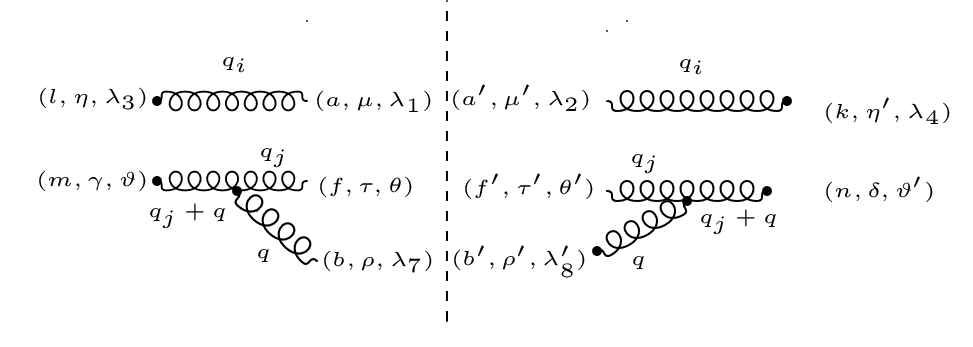
\includegraphics[width=0.95\textwidth]{images/GG/M2Squer}
\end{figure}
\begin{equation}
\begin{split}
|M_2|^2=[\frac{-i}{(q_j +q)^2}(-g_s f^{\:b\:f\:m}(g^{{\tau}{\gamma}}(-2q_j-q)^{\rho}+g^{{\gamma}{\rho}}(2q +q_j)^{\tau}+g^{{\rho}{\tau}}(q_j -q)^{\gamma})\\g_{{\tau}{{\tau}^{\prime}}}g_{{\rho}{{\rho}^{\prime}}}
(-g_s f^{\:b^{\prime}\:n\:f^{\prime}}(g^{{{\rho}^{\prime}}{{\delta}}}(-2q-q_j)^{{\tau}^{\prime}}+g^{{{\delta}}{{\tau}^{\prime}}}(2q_j +q)^{{\rho}^{\prime}}+g^{{{\tau}^{\prime}}{{\rho}^{\prime}}}(q-q_j)^{{\delta}})\frac{i}{(q_j +q)^2}][g^{{\eta}{{\eta}^{\prime}}}]
\end{split}
\end{equation}

\begin{equation}
\begin{split}
|M_2|^2=\frac{g_s^2\: f^{\:b\:f\:m} f^{\:b^{\prime}\:n\:f^{\prime}} {\delta}^{{a}{a^{\prime}}} {\delta}^{{f}{f^{\prime}}} {\delta}^{{b}{b^{\prime}}}}{(q_j +q)^2 (q_j +q)^2}[g_{{\tau}{{\tau}^{\prime}}}g_{{\rho}{{\rho}^{\prime}}}(g^{{\tau}{\gamma}}(2q_j+q)^{\rho}g^{{{\rho}^{\prime}}{{\delta}}}(2q+q_j)^{{\tau}^{\prime}}\\
-g^{{\tau}{\gamma}}(2q_j+q)^{\rho}g^{{{\delta}}{{\tau}^{\prime}}}(2q_j +q)^{{\rho}^{\prime}}-g^{{\tau}{\gamma}}(2q_j+q)^{\rho}g^{{{\tau}^{\prime}}{{\rho}^{\prime}}}(q-q_j)^{{\delta}}-g^{{\gamma}{\rho}}(2q +q_j)^{\tau}g^{{{\rho}^{\prime}}{{\delta}}}(2q+q_j)^{{\tau}^{\prime}}\\
+g^{{\gamma}{\rho}}(2q +q_j)^{\tau}g^{{{\delta}}{{\tau}^{\prime}}}(2q_j +q)^{{\rho}^{\prime}}+g^{{\gamma}{\rho}}(2q +q_j)^{\tau}g^{{{\tau}^{\prime}}{{\rho}^{\prime}}}(q-q_j)^{{\delta}}-g^{{\rho}{\tau}}(q_j -q)^{\gamma}g^{{{\rho}^{\prime}}{{\delta}}}(2q+q_j)^{{\tau}^{\prime}}\\
+g^{{\rho}{\tau}}(q_j -q)^{\gamma}g^{{{\delta}}{{\tau}^{\prime}}}(2q_j +q)^{{\rho}^{\prime}}
+g^{{\rho}{\tau}}(q_j -q)^{\gamma}g^{{{\tau}^{\prime}}{{\rho}^{\prime}}}(q-q_j)^{{\delta}}
][g^{{\eta}{{\eta}^{\prime}}}]
\end{split}
\end{equation}


\begin{equation}
\begin{split}
|M_2|^2=\frac{g_s^2\: f^{\:b\:f\:m} f^{\:b\:n\:f}}{(q_j +q)^2 (q_j +q)^2}[(2q+q_j)^{{\gamma}}(2q_j+q)^{\delta}\\
-g^{{\delta}{\gamma}}(2q_j+q)^{\rho}(2q_j +q)_{{\rho}}-(2q_j+q)^{\gamma}(q-q_j)^{{\delta}}-g^{{\delta}{\gamma}}(2q +q_j)^{\tau}(2q+q_j)_{{\tau}}\\
+(2q_j +q)^{{\gamma}}(2q +q_j)^{\delta}+(2q +q_j)^{\gamma}(q-q_j)^{{\delta}}-(q_j -q)^{\gamma}(2q+q_j)^{{\delta}}\\
+(q_j -q)^{\gamma}(2q_j +q)^{{\delta}}+d(q_j -q)^{\gamma}(q-q_j)^{{\delta}}][g^{{\eta}{{\eta}^{\prime}}}]
\end{split}
\end{equation}


\begin{equation}
\begin{split}
|M_2|^2=\frac{g_s^2\: f^{\:b\:f\:m} f^{\:b\:n\:f}}{(q_j +q)^2 (q_j +q)^2}[(3+d)q^{\gamma}{q_j}^{\delta}+(6-d)q^{\gamma}{q}^{\delta}\\+(6-d){q_j}^{\gamma}{q_j}^{\delta}+(3+d){q_j}^{\gamma}{q}^{\delta}-g^{{\delta}{\gamma}}(5{q_j}^2+5q^2+8qq_j)\\
][g^{{\eta}{{\eta}^{\prime}}}]
\end{split}
\end{equation}





\pagebreak
\subsection{One-loop corrections to the gluon self-energy diagram (Gluon-Spectator Bubble)}
\begin{figure}[h!]
\centering
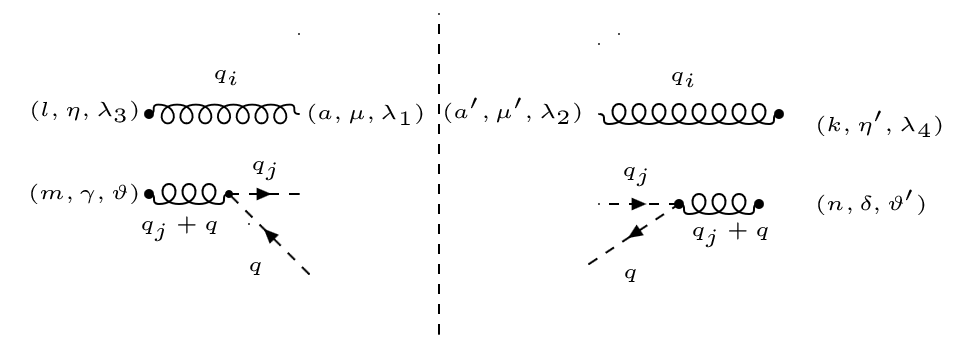
\includegraphics[width=0.95\textwidth]{images/GG/GhostM2.png}
\end{figure}
\begin{equation}
\begin{split}
{{|M_2|}^2_{Ghost \:loop}}=\frac{g_s^2 \:f^{\:b\:f\:m} f^{\:b\:n\:f}}{(q_j +q)^2 (q_j +q)^2} [-{q_j}^{{\gamma}}{q}^{{\delta}}-{q}^{{\delta}}{q_j}^{{\gamma}}][g^{{\eta}{{\eta}^{\prime}}}]
\end{split}
\end{equation}

\begin{equation}
\begin{split}
{|{M}^{\prime}_2|}^2 =\frac{g_s^2\: f^{\:b\:f\:m} f^{\:b\:n\:f}}{(q_j +q)^2 (q_j +q)^2}[(2+d)q^{\gamma}{q_j}^{\delta}+(6-d)q^{\gamma}{q}^{\delta}\\+(6-d){q_j}^{\gamma}{q_j}^{\delta}+(2+d){q_j}^{\gamma}{q}^{\delta}-g^{{\delta}{\gamma}}(8qq_j)][g^{{\eta}{{\eta}^{\prime}}}]
\end{split}
\end{equation}

\begin{equation}
\begin{split}
{|{M}^{\prime}_2|}^2 =\frac{g_s^2\: f^{\:b\:f\:m} f^{\:b\:n\:f}}{4(q_j \cdot q) (q_j \cdot q)}[-8g^{{\delta}{\gamma}}(q \cdot q_j)][g^{{\eta}{{\eta}^{\prime}}}]
\end{split}
\end{equation}

\begin{equation}
\begin{split}
{|{M}^{\prime}_2|}^2 =\frac{g_s^2\: f^{\:b\:f\:m} f^{\:b\:n\:f}}{(q_j \cdot q)}[-2g^{{\delta}{\gamma}}][g^{{\eta}{{\eta}^{\prime}}}]
\end{split}
\end{equation}

\begin{equation}
\begin{split}
{|{M}^{\prime}_2|}^2 =\frac{g_s^2\: f^{\:b\:f\:m} f^{\:b\:n\:f}}{(1-\beta_1) (1-y)\:(p_i \cdot p_k)}[-2g^{{\delta}{\gamma}}][g^{{\eta}{{\eta}^{\prime}}}]
\end{split}
\end{equation}

\section{Interference term $M_1 {M_2}^{\dagger}$}
\begin{figure}[h!]
\centering
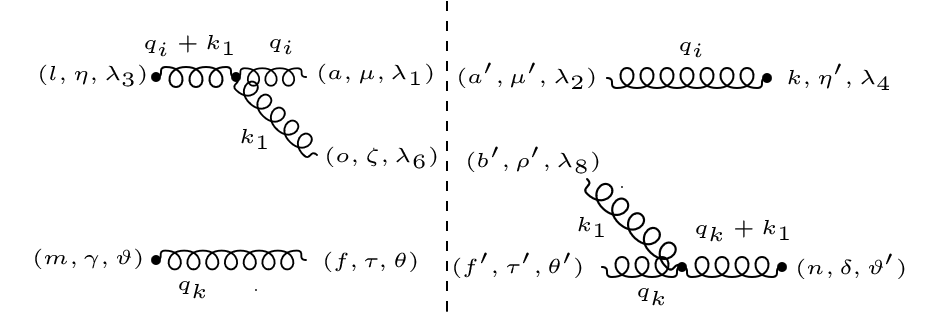
\includegraphics[width=0.95\textwidth]{images/GG/M1M2Dagger.png}
\end{figure}

\begin{equation}
\begin{split}
&M_1{M_2}^{\dagger}=[\frac{-i}{(q_i +q)^2}(-g_s f^{\:l\:a\:o}(g^{{\eta}{\mu}}(2q_i+q)^{\zeta}+g^{{\mu}{\zeta}}(q -q_i)^{\eta}-g^{{\zeta}{\eta}}(2q +q_i)^{\mu}){\varepsilon^{\lambda_1}}_{\mu} (q_i) {\varepsilon^{\lambda_6}}_{\zeta}(q)]\\
&[{{\varepsilon^{\theta}}_{{\tau}}}^* (q_j)]\\
&[\frac{i}{(q +q_j)^2}(-g_s f^{\:f^{\prime}\:b^{\prime}\:n }(g^{{{\tau}^{\prime}}{{\rho}^{\prime}}}(q_j-q)^{{\delta}}+g^{{{\rho}^{\prime}}{{\delta}}}(2q +q_j)^{{\tau}^{\prime}}-g^{{{\delta}}{{\tau}^{\prime}}}(2q_j+q)^{{\rho}^{\prime}}){{\varepsilon^{{\theta}^{\prime}}}_{{\tau}^{\prime}}}^* (q_j){{\varepsilon^{\lambda_8}}_{{\rho}^{\prime}}}^* (q)]\\
&[{{\varepsilon^{\lambda_2}}_{{\mu}^{\prime}}}^* (q_i)]
\end{split}
\end{equation}


\begin{equation}
\begin{split}
&M_1{M_2}^{\dagger}=\frac{g_s^2 f^{\:l\:a\:o} f^{\:f^{\prime}\: b^{\prime}\:n} \delta^{aa^{\prime}} \delta^{ob^{\prime}} \delta^{ff^{\prime}}}{(q_i +q)^2 (q_j +q)^2}
[{g_{{\mu}}}^{{\eta}^{\prime}} g_{{\tau}{{\tau}^{\prime}}}(g^{{\eta}{\mu}}(2q_i+q)^{\zeta}+g^{{\mu}{\zeta}}(q -q_i)^{\eta}-g^{{\zeta}{\eta}}(2q +q_i)^{\mu})\\
&g_{{{\zeta}}{{\rho}^{\prime}}}(g^{{{\tau}^{\prime}}{{\rho}^{\prime}}}(q_j-q)^{{\delta}}+g^{{{\rho}^{\prime}}{{\delta}}}(2q +q_j)^{{\tau}^{\prime}}-g^{{{\delta}}{{\tau}^{\prime}}}(2q_j+q)^{{\rho}^{\prime}}]
\end{split}
\end{equation}


\begin{equation}
\begin{split}
&M_1{M_2}^{\dagger}=\frac{g_s^2 f^{\:l\:a\:o} f^{\:f^{\prime}\: b^{\prime}\:n} \delta^{aa^{\prime}} \delta^{ob^{\prime}}\delta^{ff^{\prime}}}{(q_i +q)^2 (q_j +q)^2}\\
&[g^{{{\eta}}{{\eta}^{\prime}}}(2q_i+q)^{\gamma}(q_j-q)^{{\delta}}+g^{{{\eta}}{{\eta}^{\prime}}}(2q +q_j)^{\gamma}(2q_i+q)^{{\delta}}-g^{{{\eta}}{{\eta}^{\prime}}}g^{{{\gamma}}{{\delta}}}(2q_i+q)\cdot (2q_j+q)\\
&+g^{{{\gamma}}{{\eta}^{\prime}}}(q -q_i)^{\eta}(q_j-q)^{{\delta}}+g^{{{\eta}^{\prime}}{{\delta}}}(q -q_i)^{\eta}(2q +q_j)^{{\gamma}}
-g^{{{\gamma}}{{\delta}}}(q -q_i)^{\eta}(2q_j+q)^{{\eta}^{\prime}}\\
&-g^{{{\gamma}}{{\eta}}}(2q +q_i)^{{\eta}^{\prime}}(q_j-q)^{{\delta}}
-g^{{{\eta}}{{\delta}}}(2q +q_i)^{{\eta}^{\prime}}(2q +q_j)^{{\gamma}}
+g^{{{\gamma}}{{\delta}}}(2q_j+q)^{{\eta}}(2q +q_i)^{{\eta}^{\prime}}]\\
\end{split}
\end{equation}


\begin{equation}
\begin{split}
&M_1{M_2}^{\dagger}=\frac{g_s^2 f^{\:l\:a\:o} f^{\:f\: o\:n}}{4(q \cdot q_i) (q \cdot q_j)}\\
&\lbrace g^{{{\eta}}{{\eta}^{\prime}}}[2{q_i}^{{\gamma}}{q_j}^{\delta}+2{q_i}^{{\gamma}}{q}^{\delta}+{q}^{{\gamma}}{q_j}^{\delta}+{q}^{{\gamma}}{q}^{\delta}+4q^{{\gamma}}{q_i}^{\delta}+2q^{{\gamma}}{q}^{\delta}+2{q_j}^{{\gamma}}{q_i}^{\delta}+{q_j}^{{\gamma}}{q}^{\delta}]\\
&-g^{{{\eta}}{{\eta}^{\prime}}}g^{{{\gamma}}{{\delta}}}(2q\cdot q_j+ q\cdot q+4q_i \cdot q_j+2q_i \cdot q)+g^{{{\gamma}}{{\eta}^{\prime}}}[{q}^{{\eta}}{q_j}^{\delta}-{q}^{{\eta}}{q}^{\delta}-{q_i}^{{\eta}}{q_j}^{\delta}+{q_i}^{{\eta}}{q}^{\delta}]\\
&+g^{{{\eta}^{\prime}}{{\delta}}}[2{q}^{{\eta}}{q}^{\gamma}+{q}^{{\eta}}{q_j}^{\gamma}+{q_i}^{{\eta}}{q}^{\gamma}+{q_i}^{{\eta}}{q_j}^{\gamma}]-g^{{{\gamma}}{{\delta}}}[2{q}^{\eta}{q_j}^{{\eta}^{\prime}}+{q}^{\eta}{q}^{{\eta}^{\prime}}-2{q_i}^{\eta}{q_j}^{{\eta}^{\prime}}-{q_i}^{\eta}{q}^{{\eta}^{\prime}}]\\
&-g^{{{\gamma}}{{\eta}}}[2{q}^{{\eta}^{\prime}}{q_j}^{{\delta}}-{2q}^{{\eta}^{\prime}}{q}^{{\delta}}+{q_i}^{{\eta}^{\prime}}{q_j}^{{\delta}}-{q_i}^{{\eta}^{\prime}}{q}^{{\delta}}]-g^{{{\eta}}{{\delta}}}[4{q}^{{\eta}^{\prime}}{q}^{{\gamma}}+2{q}^{{\eta}^{\prime}}{q_j}^{{\gamma}}+2{q_i}^{{\eta}^{\prime}}{q}^{{\gamma}}+{q_i}^{{\eta}^{\prime}}{q_j}^{{\gamma}}]\\
&+g^{{{\gamma}}{{\delta}}}[4{q_j}^{{\eta}}{q}^{{\eta}^{\prime}}+2{q_j}^{{\eta}}{q_i}^{{\eta}^{\prime}}+{q}^{{\eta}}{q}^{{\eta}^{\prime}}+{q}^{{\eta}}{q_i}^{{\eta}^{\prime}}]\rbrace
\end{split}
\end{equation}



\begin{equation}
\begin{split}
{k_1}^{{\eta}}{k_1}^{{\eta}^{\prime}}&=[(1-\beta_1)^2-y^2 {\beta_1}^2 (\frac{Q^2}{2p_i \cdot Q})^2] {p_i}^{{\eta}}{p_i}^{{\eta}^{\prime}}-y^2 {\beta_1}^2 (\frac{Q^2}{2p_i \cdot Q}){p_i}^{{\eta}}{Q}^{{\eta}^{\prime}}-y^2 {\beta_1}^2 (\frac{Q^2}{2p_i \cdot Q}){Q}^{{\eta}}{p_i}^{{\eta}^{\prime}}\\
{k_1}^{{\eta}}{q_i}^{{\eta}^{\prime}}&=[\beta_1(1-\beta_1)-y {\beta_1}^2 (\frac{Q^2}{2p_i \cdot Q})] {p_i}^{{\eta}}{p_i}^{{\eta}^{\prime}}+y {\beta_1}^2 {Q}^{{\eta}}{p_i}^{{\eta}^{\prime}}\\
{q_i}^{{\eta}}{k_1}^{{\eta}^{\prime}}&=[\beta_1(1-\beta_1)-y {\beta_1}^2 (\frac{Q^2}{2p_i \cdot Q})] {p_i}^{{\eta}}{p_i}^{{\eta}^{\prime}}+y {\beta_1}^2 {p_i}^{{\eta}}{Q}^{{\eta}^{\prime}}\\
{q_i}^{{\eta}}{q_i}^{{\eta}^{\prime}}&={\beta_1}^2 {p_i}^{{\eta}}{p_i}^{{\eta}^{\prime}}\\
{k_1}^{{\eta}}{q_k}^{{\eta}^{\prime}}&= [(1-\beta_1)-y\beta_1 (\frac{Q^2}{2p_i \cdot Q})] \sqrt{1-y}{p_i}^{{\eta}}{{p_k}^{{\eta}^{\prime}}}-y {\beta_1} (\frac{Q^2}{2p_i \cdot Q}) A_1 \:{p_i}^{{\eta}}{p_i}^{{\eta}^{\prime}}
-y {\beta_1} (\frac{Q^2}{2p_i \cdot Q}) A_2\: {p_i}^{{\eta}}{Q}^{{\eta}^{\prime}}\\
&+y {\beta_1} A_1 \:{Q}^{{\eta}}{p_i}^{{\eta}^{\prime}}+y {\beta_1} A_2 \:{Q}^{{\eta}}{Q}^{{\eta}^{\prime}}+y {\beta_1}\sqrt{1-y}{Q}^{{\eta}}{{p_k}^{{\eta}^{\prime}}}\\
{q_i}^{{\eta}}{q_k}^{{\eta}^{\prime}}&=A_1\beta_1 {p_i}^{{\eta}}{{p_i}^{{\eta}^{\prime}}}+A_2\beta_1 {p_i}^{{\eta}}{{Q}^{{\eta}^{\prime}}}+\beta_1 \sqrt{1-y}{p_i}^{{\eta}}{{p_k}^{{\eta}^{\prime}}}\\
{q_k}^{\eta}{k_1}^{{{\eta}}^{\prime}}&=[(1-\beta_1)-y\beta_1 (\frac{Q^2}{2p_i \cdot Q})] \sqrt{1-y}{p_k}^{{\eta}}{{p_i}^{{\eta}^{\prime}}}-y {\beta_1} (\frac{Q^2}{2p_i \cdot Q}) A_1 \:{p_i}^{{\eta}}{p_i}^{{\eta}^{\prime}}
-y {\beta_1} (\frac{Q^2}{2p_i \cdot Q}) A_2\: {Q}^{{\eta}}{p_i}^{{\eta}^{\prime}}\\
&+y {\beta_1} A_1 \:{p_i}^{{\eta}}{Q}^{{\eta}^{\prime}}+y {\beta_1} A_2 \:{Q}^{{\eta}}{Q}^{{\eta}^{\prime}}+y {\beta_1}\sqrt{1-y}{p_k}^{{\eta}}{{Q}^{{\eta}^{\prime}}}\\
{q_k}^{\eta}{q_i}^{{{\eta}}^{\prime}}&=A_1\beta_1 {p_i}^{{\eta}}{{p_i}^{{\eta}^{\prime}}}+A_2\beta_1 {Q}^{{\eta}}{{p_i}^{{\eta}^{\prime}}}+\beta_1 \sqrt{1-y}{p_k}^{{\eta}}{{p_i}^{{\eta}^{\prime}}}\\
\end{split}
\end{equation}

\subsection*{Calculation of the first Term}

\begin{equation}
\begin{split} 
& g^{{{\eta}}{{\eta}^{\prime}}}[2\lbrace A_1\beta_1 {p_i}^{{\gamma}}{{p_i}^{{\delta}}}+A_2\beta_1 {p_i}^{{\gamma}}{{Q}^{{\delta}}}+\beta_1 \sqrt{1-y}{p_i}^{{\gamma}}{{p_k}^{{\delta}}} \rbrace \\&
+2\lbrace [\beta_1(1-\beta_1)-y {\beta_1}^2 (\frac{Q^2}{2p_i \cdot Q})] {p_i}^{{\gamma}}{p_i}^{{\delta}}+y {\beta_1}^2 {p_i}^{{\gamma}}{Q}^{{\delta}} \rbrace\\
&+\lbrace [(1-\beta_1)-y\beta_1 (\frac{Q^2}{2p_i \cdot Q})] \sqrt{1-y}{p_i}^{{\gamma}}{{p_k}^{{\delta}}}-y {\beta_1} (\frac{Q^2}{2p_i \cdot Q}) A_1 \:{p_i}^{{\gamma}}{p_i}^{{\delta}}
-y {\beta_1} (\frac{Q^2}{2p_i \cdot Q}) A_2\: {p_i}^{{\gamma}}{Q}^{{\delta}}\\
&+y {\beta_1} A_1 \:{Q}^{{\gamma}}{p_i}^{{\delta}}+y {\beta_1} A_2 \:{Q}^{{\gamma}}{Q}^{{\delta}}+y {\beta_1}\sqrt{1-y}{Q}^{{\gamma}}{{p_k}^{{\delta}}} \rbrace \\
&+3\lbrace [(1-\beta_1)^2-y^2 {\beta_1}^2 (\frac{Q^2}{2p_i \cdot Q})^2] {p_i}^{{\gamma}}{p_i}^{{\delta}}-y^2 {\beta_1}^2 (\frac{Q^2}{2p_i \cdot Q}){p_i}^{{\gamma}}{Q}^{{\delta}}-y^2 {\beta_1}^2 (\frac{Q^2}{2p_i \cdot Q}){Q}^{{\gamma}}{p_i}^{{\delta}} \rbrace\\
&+4\lbrace [\beta_1(1-\beta_1)-y {\beta_1}^2 (\frac{Q^2}{2p_i \cdot Q})] {p_i}^{{\gamma}}{p_i}^{{\delta}}+y {\beta_1}^2 {Q}^{{\gamma}}{p_i}^{{\delta}} \rbrace\\
&+2\lbrace A_1\beta_1 {p_i}^{{\gamma}}{{p_i}^{{\delta}}}+A_2\beta_1 {Q}^{{\gamma}}{{p_i}^{{\delta}}}+\beta_1 \sqrt{1-y}{p_k}^{{\gamma}}{{p_i}^{{\delta}}} \rbrace \\
&+\lbrace [(1-\beta_1)-y\beta_1 (\frac{Q^2}{2p_i \cdot Q})] \sqrt{1-y}{p_k}^{{\gamma}}{{p_i}^{{\delta}}}-y {\beta_1} (\frac{Q^2}{2p_i \cdot Q}) A_1 \:{p_i}^{{\gamma}}{p_i}^{{\delta}}
-y {\beta_1} (\frac{Q^2}{2p_i \cdot Q}) A_2\: {Q}^{{\gamma}}{p_i}^{{\delta}}\\
&+y {\beta_1} A_1 \:{p_i}^{{\gamma}}{Q}^{{\delta}}+y {\beta_1} A_2 \:{Q}^{{\gamma}}{Q}^{{\delta}}+y {\beta_1}\sqrt{1-y}{p_k}^{{\gamma}}{{Q}^{{\delta}}} \rbrace]\\
\end{split}
\end{equation}

\begin{equation}
\begin{split} 
& g^{{{\eta}}{{\eta}^{\prime}}}\lbrace [2 A_1\beta_1+2 [\beta_1(1-\beta_1)-y {\beta_1}^2 (\frac{Q^2}{2p_i \cdot Q})]\\
&+4 [\beta_1(1-\beta_1)-y {\beta_1}^2 (\frac{Q^2}{2p_i \cdot Q})]+3 [(1-\beta_1)^2-y^2 {\beta_1}^2 (\frac{Q^2}{2p_i \cdot Q})^2]\\
&+2 A_1\beta_1 -y {\beta_1} (\frac{Q^2}{2p_i \cdot Q}) A_1\:-y {\beta_1} (\frac{Q^2}{2p_i \cdot Q}) A_1 \:] {p_i}^{{\gamma}}{{p_i}^{{\delta}}}\\
&+[2A_2\beta_1+2y {\beta_1}^2 -y {\beta_1} (\frac{Q^2}{2p_i \cdot Q}) A_2\: -3y^2 {\beta_1}^2 (\frac{Q^2}{2p_i \cdot Q})+y {\beta_1} A_1] {p_i}^{{\gamma}}{{Q}^{{\delta}}}\\
&+[2\beta_1+[(1-\beta_1)-y\beta_1 (\frac{Q^2}{2p_i \cdot Q})] ] \sqrt{1-y}{p_i}^{{\gamma}}{{p_k}^{{\delta}}} \\
&+[y {\beta_1} A_1+4y {\beta_1}^2 +2A_2\beta_1 -3y^2 {\beta_1}^2 (\frac{Q^2}{2p_i \cdot Q})-y {\beta_1} (\frac{Q^2}{2p_i \cdot Q}) A_2\: ] \:{Q}^{{\gamma}}{p_i}^{{\delta}}\\
&+[y {\beta_1} A_2+y {\beta_1} A_2] \:{Q}^{{\gamma}}{Q}^{{\delta}}+y {\beta_1}\sqrt{1-y}{Q}^{{\gamma}}{{p_k}^{{\delta}}} \\
&+[2\beta_1 + [(1-\beta_1)-y\beta_1 (\frac{Q^2}{2p_i \cdot Q})] ]\sqrt{1-y}{p_k}^{{\gamma}}{{p_i}^{{\delta}}}+y {\beta_1}\sqrt{1-y}{p_k}^{{\gamma}}{{Q}^{{\delta}}}\rbrace\\
\end{split}
\end{equation}

\subsection*{Calculation of the second term}

\begin{equation}
\begin{split}
&{\color[RGB]{255,0,0} -g^{{{\eta}}{{\eta}^{\prime}}}g^{{{\gamma}}{{\delta}}}}\lbrace [2[(1-\beta_1)-y\beta_1 (\frac{Q^2}{2p_i \cdot Q})]+4\beta_1] \sqrt{1-y}\:({p_i}\cdot{p_k})\\
&+[-2y {\beta_1} (\frac{Q^2}{2p_i \cdot Q}) A_2+4A_2\beta_1 +2y {\beta_1}^2 -y^2 {\beta_1}^2 (\frac{Q^2}{2p_i \cdot Q})]\: ({p_i}\cdot{Q})\\
&+[2y {\beta_1} A_1-y^2 {\beta_1}^2 (\frac{Q^2}{2p_i \cdot Q})] \:({Q}\cdot{p_i})+2y {\beta_1} A_2 \:({Q}\cdot{Q})+2y {\beta_1}\sqrt{1-y}\:({Q}\cdot{p_k})\rbrace
\end{split}
\end{equation}

In terms of collinear case:
\begin{equation}
\begin{split}
y\rightarrow 0
\end{split}
\end{equation}

\begin{equation}
\begin{split}
&{\color[RGB]{255,0,0} -g^{{{\eta}}{{\eta}^{\prime}}}g^{{{\gamma}}{{\delta}}}}\lbrace [2(1-\beta_1)+4\beta_1] \sqrt{1-y}\:({p_i}\cdot{p_k})\rbrace
\end{split}
\end{equation}


\subsection*{Calculation of the third term}
\begin{equation}
\begin{split} 
&+g^{{{\gamma}}{{\eta}^{\prime}}}\lbrace [(1-\beta_1)-y\beta_1 (\frac{Q^2}{2p_i \cdot Q})] \sqrt{1-y}{p_i}^{{\eta}}{{p_k}^{{\delta}}}-y {\beta_1} (\frac{Q^2}{2p_i \cdot Q}) A_1 \:{p_i}^{{\eta}}{p_i}^{{\delta}}
-y {\beta_1} (\frac{Q^2}{2p_i \cdot Q}) A_2\: {p_i}^{{\eta}}{Q}^{{\eta}^{\prime}}\\
&+y {\beta_1} A_1 \:{Q}^{{\eta}}{p_i}^{{\delta}}+y {\beta_1} A_2 \:{Q}^{{\eta}}{Q}^{{\delta}}+y {\beta_1}\sqrt{1-y}{Q}^{{\eta}}{{p_k}^{{\delta}}}\\
&-[[(1-\beta_1)^2-y^2 {\beta_1}^2 (\frac{Q^2}{2p_i \cdot Q})^2] {p_i}^{{\eta}}{p_i}^{{\delta}}-y^2 {\beta_1}^2 (\frac{Q^2}{2p_i \cdot Q}){p_i}^{{\eta}}{Q}^{{\delta}}-y^2 {\beta_1}^2 (\frac{Q^2}{2p_i \cdot Q}){Q}^{{\eta}}{p_i}^{{\delta}}]\\
&-[A_1\beta_1 {p_i}^{{\eta}}{{p_i}^{{\delta}}}+A_2\beta_1 {p_i}^{{\eta}}{{Q}^{{\delta}}}+\beta_1 \sqrt{1-y}{p_i}^{{\eta}}{{p_k}^{{\delta}}}]\\
&+[\beta_1(1-\beta_1)-y {\beta_1}^2 (\frac{Q^2}{2p_i \cdot Q})] {p_i}^{{\eta}}{p_i}^{{\eta}^{\prime}}+y {\beta_1}^2 {p_i}^{{\eta}}{Q}^{{\eta}^{\prime}}\rbrace\\
\end{split}
\end{equation}

\subsection*{Calculation of the fourth term}

\begin{equation}
\begin{split} 
&+g^{{{\eta}^{\prime}}{{\delta}}}\lbrace [(1-\beta_1)-y\beta_1 (\frac{Q^2}{2p_i \cdot Q})-\beta_1] \sqrt{1-y}{p_i}^{{\eta}}{{p_k}^{{\gamma}}}\\
&+[2[(1-\beta_1)^2-y^2 {\beta_1}^2 (\frac{Q^2}{2p_i \cdot Q})^2]-y {\beta_1} (\frac{Q^2}{2p_i \cdot Q}) A_1 +A_1\beta_1 +\\
&[\beta_1(1-\beta_1)-y {\beta_1}^2 (\frac{Q^2}{2p_i \cdot Q})]] {p_i}^{{\eta}}{p_i}^{{\gamma}}\\
& +[-2y^2 {\beta_1}^2 (\frac{Q^2}{2p_i \cdot Q})-y {\beta_1} (\frac{Q^2}{2p_i \cdot Q}) A_2\:+A_2\beta_1 +y {\beta_1}^2] {p_i}^{{\eta}}{Q}^{{\gamma}}\\
&+[y {\beta_1} A_1 \:+2y^2 {\beta_1}^2 (\frac{Q^2}{2p_i \cdot Q})]{Q}^{{\eta}}{p_i}^{{\gamma}}+y {\beta_1} A_2 \:{Q}^{{\eta}}{Q}^{{\gamma}}+y {\beta_1}\sqrt{1-y}{Q}^{{\eta}}{{p_k}^{{\gamma}}}
\rbrace\\
\end{split}
\end{equation}

\subsection*{Calculation of the fifth term}

\begin{equation}
\begin{split} 
&-g^{{{\gamma}}{{\delta}}}\lbrace[2[(1-\beta_1)-y\beta_1 (\frac{Q^2}{2p_i \cdot Q})]-2\beta_1] \sqrt{1-y}{p_i}^{{\eta}}{{p_k}^{{\eta}^{\prime}}}\\
&[-2y {\beta_1} (\frac{Q^2}{2p_i \cdot Q}) A_1+[(1-\beta_1)^2-y^2 {\beta_1}^2 (\frac{Q^2}{2p_i \cdot Q})^2]-2A_1\beta_1\\
&-[\beta_1(1-\beta_1)-y {\beta_1}^2 (\frac{Q^2}{2p_i \cdot Q})] ]\:{p_i}^{{\eta}}{p_i}^{{\eta}^{\prime}}\\
&[-2y {\beta_1} (\frac{Q^2}{2p_i \cdot Q}) A_2\: -y^2 {\beta_1}^2 (\frac{Q^2}{2p_i \cdot Q})-y {\beta_1}^2 -2A_2\beta_1 ]{p_i}^{{\eta}}{Q}^{{\eta}^{\prime}}\\
&+[2y {\beta_1} A_1-y^2 {\beta_1}^2 (\frac{Q^2}{2p_i \cdot Q})] \:{Q}^{{\eta}}{p_i}^{{\eta}^{\prime}}+2y {\beta_1} A_2 \:{Q}^{{\eta}}{Q}^{{\eta}^{\prime}}+2y {\beta_1}\sqrt{1-y}{Q}^{{\eta}}{{p_k}^{{\eta}^{\prime}}}\rbrace\\
\end{split}
\end{equation}

\subsection*{Calculation of the sixth term}
\begin{equation}
\begin{split}
&-g^{{{\gamma}}{{\eta}}}\lbrace[2[(1-\beta_1)-y\beta_1 (\frac{Q^2}{2p_i \cdot Q})]+\beta_1 ] \sqrt{1-y}{p_i}^{{\eta}^{\prime}}{{p_k}^{{\delta}}}\\
&[-2y {\beta_1} (\frac{Q^2}{2p_i \cdot Q}) A_1-2[(1-\beta_1)^2-y^2 {\beta_1}^2 (\frac{Q^2}{2p_i \cdot Q})^2]\\
&-[\beta_1(1-\beta_1)-y {\beta_1}^2 (\frac{Q^2}{2p_i \cdot Q})] +A_1\beta_1 ] \:{p_i}^{{\eta}^{\prime}}{p_i}^{{\delta}}\\
&[-2y {\beta_1} (\frac{Q^2}{2p_i \cdot Q}) A_2\:+2y^2 {\beta_1}^2 (\frac{Q^2}{2p_i \cdot Q})+A_2\beta_1 -y {\beta_1}^2 ] {p_i}^{{\eta}^{\prime}}{Q}^{{\delta}}\\
&+[2y {\beta_1} A_1+2y^2 {\beta_1}^2 (\frac{Q^2}{2p_i \cdot Q})] \:{Q}^{{\eta}^{\prime}}{p_i}^{{\delta}}+2y {\beta_1} A_2 \:{Q}^{{\eta}^{\prime}}{Q}^{{\delta}}+2y {\beta_1}\sqrt{1-y}{Q}^{{\eta}^{\prime}}{{p_k}^{{\delta}}}
\rbrace
\end{split}
\end{equation}

\subsection*{Calculation of the seventh term}

\begin{equation}
\begin{split} 
&-g^{{{\eta}}{{\delta}}}\lbrace [2[(1-\beta_1)-y\beta_1 (\frac{Q^2}{2p_i \cdot Q})]+\beta_1 ] \sqrt{1-y}{p_i}^{{\eta}^{\prime}}{{p_k}^{{\gamma}}}\\
&[4[(1-\beta_1)^2-y^2 {\beta_1}^2 (\frac{Q^2}{2p_i \cdot Q})^2]-2y {\beta_1} (\frac{Q^2}{2p_i \cdot Q}) A_1 +A_1\beta_1 \\
&+2[\beta_1(1-\beta_1)-y {\beta_1}^2 (\frac{Q^2}{2p_i \cdot Q})]] {p_i}^{{\eta}^{\prime}}{p_i}^{{\gamma}}\\
&+[-4y^2 {\beta_1}^2 (\frac{Q^2}{2p_i \cdot Q})-2y {\beta_1} (\frac{Q^2}{2p_i \cdot Q}) A_2\: +2y {\beta_1}^2 +A_2\beta_1 ]{p_i}^{{\eta}^{\prime}}{Q}^{{\gamma}}\\
&+[-4y^2 {\beta_1}^2 (\frac{Q^2}{2p_i \cdot Q})+2y {\beta_1} A_1]{Q}^{{\eta}}{p_i}^{{\eta}^{\prime}}+2y {\beta_1} A_2 \:{Q}^{{\eta}}{Q}^{{\eta}^{\prime}}+2y {\beta_1}\sqrt{1-y}{Q}^{{\eta}^{\prime}}{{p_k}^{{\gamma}}}\rbrace\\
\end{split}
\end{equation}

\subsection*{Calculation of the eighth term}

\begin{equation}
\begin{split} 
&+g^{{{\gamma}}{{\delta}}}\lbrace
[4[(1-\beta_1)-y\beta_1 (\frac{Q^2}{2p_i \cdot Q})] +2\beta_1]\sqrt{1-y}{p_k}^{{\eta}}{{p_i}^{{\eta}^{\prime}}}\\
&+[-4y {\beta_1} (\frac{Q^2}{2p_i \cdot Q}) A_1+2A_1\beta_1 +[\beta_1(1-\beta_1)-y {\beta_1}^2 (\frac{Q^2}{2p_i \cdot Q})]\\
&+[(1-\beta_1)^2-y^2 {\beta_1}^2 (\frac{Q^2}{2p_i \cdot Q})^2]] \:{p_i}^{{\eta}}{p_i}^{{\eta}^{\prime}}\\
&+[4y {\beta_1} A_1 -y^2 {\beta_1}^2 (\frac{Q^2}{2p_i \cdot Q})]\:{p_i}^{{\eta}}{Q}^{{\eta}^{\prime}}+4y {\beta_1} A_2 \:{Q}^{{\eta}}{Q}^{{\eta}^{\prime}}+4y {\beta_1}\sqrt{1-y}{p_k}^{{\eta}}{{Q}^{{\eta}^{\prime}}}\\
&+[2A_2\beta_1-4y {\beta_1} (\frac{Q^2}{2p_i \cdot Q}) A_2\:-y^2 {\beta_1}^2 (\frac{Q^2}{2p_i \cdot Q})+y {\beta_1}^2] {Q}^{{\eta}}{{p_i}^{{\eta}^{\prime}}}\rbrace
\end{split}
\end{equation}

\subsection*{Final result}
\begin{equation}
\begin{split}
&M_1{M_2}^{\dagger}=\frac{g_s^2 C_A}{4y(1-\beta_1) (1-y)\:(p_i \cdot p_k)(p_i \cdot Q)}
g^{{{\eta}}{{\eta}^{\prime}}}g^{{{\gamma}}{{\delta}}} [-2(1-\beta_1)-4\beta_1] \sqrt{1-y}\:({p_i}\cdot{p_k})\\\\
&\Rightarrow \:\:\:\:\:\:\:\:\:\:\:\:\:\:\:\:\:\:\:\:\:\:\:\:\:M_1{M_2}^{\dagger}=\frac{(-1-\beta_1)\sqrt{1-y}}{2(1-\beta_1)(1-y)}\:\:\frac{g_s^2 C_A}{y (p_i \cdot Q)}
g^{{{\eta}}{{\eta}^{\prime}}}g^{{{\gamma}}{{\delta}}}  \\
\end{split}
\end{equation}



\pagebreak

\section{Interference term $M_1 {M_2}^{\dagger} for the inverse case $}
\begin{figure}[h!]
\centering
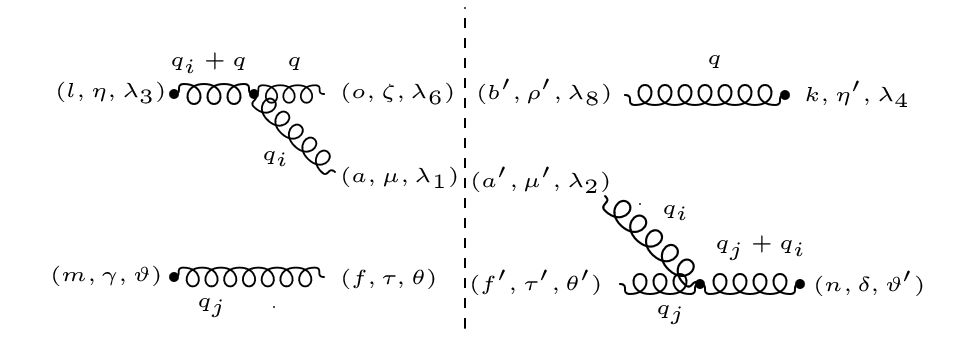
\includegraphics[width=0.95\textwidth]{images/GG/M1DaggerggInverse.png}
\end{figure}

\begin{equation}
\begin{split}
&M_1{M_2}^{\dagger}=[\frac{-i}{(q_i +q)^2}(-g_s f^{\:l\:a\:o}(g^{{\eta}{\mu}}(2q_i+q)^{\zeta}+g^{{\mu}{\zeta}}(q -q_i)^{\eta}-g^{{\zeta}{\eta}}(2q +q_i)^{\mu}){\varepsilon^{\lambda_1}}_{\mu} (q_i) {\varepsilon^{\lambda_6}}_{\zeta}(q)]\\
&[{{\varepsilon^{\theta}}_{{\tau}}}^* (q_j)]\\
&[\frac{i}{(q +q_j)^2}(-g_s f^{\:f^{\prime}\:b^{\prime}\:n }(g^{{{\tau}^{\prime}}{{\rho}^{\prime}}}(q_j-q)^{{\delta}}+g^{{{\rho}^{\prime}}{{\delta}}}(2q +q_j)^{{\tau}^{\prime}}-g^{{{\delta}}{{\tau}^{\prime}}}(2q_j+q)^{{\rho}^{\prime}}){{\varepsilon^{{\theta}^{\prime}}}_{{\tau}^{\prime}}}^* (q_j){{\varepsilon^{\lambda_8}}_{{\rho}^{\prime}}}^* (q)]\\
&[{{\varepsilon^{\lambda_2}}_{{\mu}^{\prime}}}^* (q_i)]
\end{split}
\end{equation}


\begin{equation}
\begin{split}
&M_1{M_2}^{\dagger}=\frac{g_s^2 f^{\:l\:a\:o} f^{\:f^{\prime}\: b^{\prime}\:n} \delta^{aa^{\prime}} \delta^{ob^{\prime}} \delta^{ff^{\prime}}}{(q_i +q)^2 (q_j +q)^2}
[{g_{{\mu}}}^{{\eta}^{\prime}} g_{{\tau}{{\tau}^{\prime}}}(g^{{\eta}{\mu}}(2q_i+q)^{\zeta}+g^{{\mu}{\zeta}}(q -q_i)^{\eta}-g^{{\zeta}{\eta}}(2q +q_i)^{\mu})\\
&g_{{{\zeta}}{{\rho}^{\prime}}}(g^{{{\tau}^{\prime}}{{\rho}^{\prime}}}(q_j-q)^{{\delta}}+g^{{{\rho}^{\prime}}{{\delta}}}(2q +q_j)^{{\tau}^{\prime}}-g^{{{\delta}}{{\tau}^{\prime}}}(2q_j+q)^{{\rho}^{\prime}}]
\end{split}
\end{equation}




\section{$|M^{2}|$}































\chapter{Quark gluon quark emission kernel}

\begin{figure}[ht!]
\centering
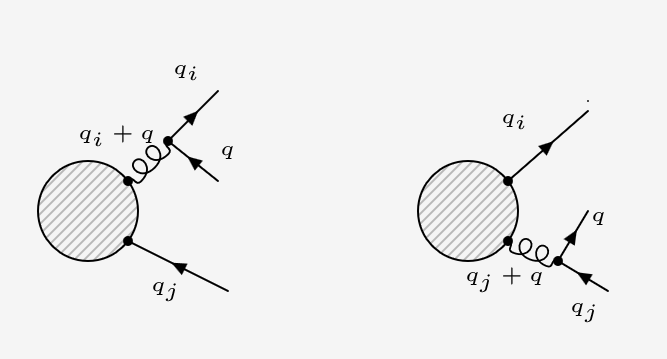
\includegraphics[width=0.85\textwidth]{images/QG/QGDiagrams.png}
\end{figure}

This case concerns a daughter quark from a parent gluon which splits into a quark-anti-quark pair. Here no singularity develops since daughter and parent can always be distinguished.\\
This is the reason why the calculation is not mentioned here, because the evaluation is analogous to the other parts considered so far.
\pagebreak
%
%\section{Quark loop}
%\begin{figure}[ht!]
%\centering
%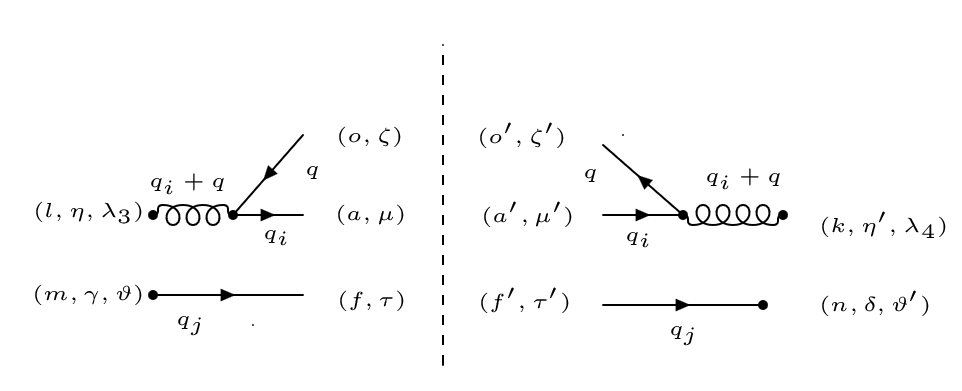
\includegraphics[scale=0.7]{images/QG/M1Squer.png}
%\end{figure}
%
%\begin{equation}
%\begin{split}
%|M_1|^2=[\frac{-i}{(q_i +k_1)^2}\not{q_i}(-ig_s {\gamma}^{\eta}\times{[T^l]_a}^o)\not{q}(ig_s {\gamma}^{{\eta}^{\prime}}\times{[T^k]_{o^{\prime}}}^{a^{\prime}})\frac{i}{(q_i +k_1)^2}][\not{q_k}]
%\end{split}
%\end{equation}
%
%
%\begin{equation}
%\begin{split}
%|M_1|^2=\frac{{g_s}^2 {[T^l]_a}^o {[T^k]_{o^{\prime}}}^{a^{\prime}}}{4(k_1 \cdot q_i)(k_1 \cdot q_i)}[ {k_1}_{\alpha} {q_i}_{\mu}\:(\gamma^{\mu}{\gamma}^{\eta}\gamma^{\alpha}\: {\gamma}^{{\eta}^{\prime}})][\not{q_k}]
%\end{split}
%\end{equation}
%
%
%\begin{equation}
%\begin{split}
%|M_1|^2=\frac{{g_s}^2 {[T^l]_a}^o {[T^k]_{o^{\prime}}}^{a^{\prime}}}{4(k_1 \cdot q_i)(k_1 \cdot q_i)}[{q_i}_{\mu}{k_1}_{\alpha}\:(2g^{{\eta}{\mu}}-{\gamma}^{\eta}\gamma^{\mu})\gamma_{\alpha}\: {\gamma}^{{\eta}^{\prime}}][\not{q_k}]
%\end{split}
%\end{equation}
%
%\begin{equation}
%\begin{split}
%|M_1|^2=\frac{{g_s}^2 {[T^l]_a}^o {[T^k]_{o^{\prime}}}^{a^{\prime}}}{4(k_1 \cdot q_i)(k_1 \cdot q_i)}[(2{q_i}^{\eta}\not{k_1}\:-{\gamma}^{\eta}\not{q_i}\not{k_1})\: {\gamma}^{{\eta}^{\prime}}][\not{q_k}]
%\end{split}
%\end{equation}
%
%\begin{equation}
%\begin{split}
%|M_1|^2=\frac{{g_s}^2 {[T^l]_a}^o {[T^k]_{o^{\prime}}}^{a^{\prime}}}{4(k_1 \cdot q_i)(k_1 \cdot q_i)}[(2{q_i}^{\eta}\not{k_1}\:-{\gamma}^{\eta}\not{q_i}\not{k_1})\: {g}^{{\eta}^{\prime} \eta} \gamma_{\eta}][\not{q_k}]
%\end{split}
%\end{equation}
%
%\begin{equation}
%\begin{split}
%|M_1|^2=\frac{{g_s}^2 {[T^l]_a}^o {[T^k]_{o^{\prime}}}^{a^{\prime}}}{4(k_1 \cdot q_i)(k_1 \cdot q_i)}(2{q_i}^{\eta}\not{k_1}\gamma_{\eta}\:-{\gamma}^{\eta}\not{q_i}\not{k_1}\gamma_{\eta})\: [{g}^{{\eta}^{\prime} \eta} ][\not{q_k}]
%\end{split}
%\end{equation}
%
%\begin{equation}
%\begin{split}
%|M_1|^2=\frac{{g_s}^2 {[T^l]_a}^o {[T^k]_{o^{\prime}}}^{a^{\prime}}}{4(k_1 \cdot q_i)(k_1 \cdot q_i)}(2\not{k_1}\not{q_i}\:-{q_i}_{\mu} {k_1}_{\alpha}{\gamma}^{\eta}{\gamma}^{\mu}{\gamma}^{\alpha}\gamma_{\eta})\: [{g}^{{\eta}^{\prime} \eta} ][\not{q_k}]
%\end{split}
%\end{equation}
%
%\begin{equation}
%\begin{split}
%|M_1|^2=\frac{{g_s}^2 {[T^l]_a}^o {[T^k]_{o^{\prime}}}^{a^{\prime}}}{4(k_1 \cdot q_i)(k_1 \cdot q_i)}(2\not{k_1}\not{q_i}\:-{q_i}_{\mu} {k_1}_{\alpha}(4g^{\alpha \mu}))\: [{g}^{{\eta}^{\prime} \eta} ][\not{q_k}]
%\end{split}
%\end{equation}
%
%\begin{equation}
%\begin{split}
%|M_1|^2=\frac{{g_s}^2 {[T^l]_a}^o {[T^k]_{o^{\prime}}}^{a^{\prime}}}{4(k_1 \cdot q_i)(k_1 \cdot q_i)}(2\not{k_1}\not{q_i}\:-4({q_i} \cdot {k_1}))\: [{g}^{{\eta}^{\prime} \eta} ][\not{q_k}]
%\end{split}
%\end{equation}
%
%\begin{equation}
%\begin{split}
%&|M_1|^2=\frac{{g_s}^2 {[T^l]_a}^o {[T^k]_{o^{\prime}}}^{a^{\prime}}}{4y^2\:(p_i\cdot Q)(p_i\cdot Q) }\\&
%(2(\zeta_1 \not{p_i} + \lambda_1\not{Q} + \sqrt{y\alpha_1\beta_1}\not{n}_{\bot,1} )( \zeta_q\not{p_i} + \lambda_q\not{Q} - \sqrt{y\alpha_1\beta_1}\not{n}_{\bot,l})-4y\:(p_i\cdot Q ))\: [{g}^{{\eta}^{\prime} \eta} ][\not{q_k}]
%\end{split}
%\end{equation}
%
%\begin{equation}
%\begin{split}
%&|M_1|^2=\frac{{g_s}^2 {[T^l]_a}^o {[T^k]_{o^{\prime}}}^{a^{\prime}}}{4y^2\:(p_i\cdot Q)(p_i\cdot Q) }\\&
%(2\zeta_1\lambda_q \not{p_i}\not{Q} +2\lambda_1\zeta_q\not{Q}\not{p_i} - 2{y\alpha_1\beta_1}{{n}_{\bot,1}}^2-4y\:(p_i\cdot Q ))\: [{g}^{{\eta}^{\prime} \eta} ][\not{q_k}]
%\end{split}
%\end{equation}
%
%\begin{equation}
%\begin{split}
%&|M_1|^2=\frac{{g_s}^2 {[T^l]_a}^o {[T^k]_{o^{\prime}}}^{a^{\prime}}}{4y^2\:(p_i\cdot Q)(p_i\cdot Q) }\\&
%(2y\alpha_1^2 \not{p_i}\not{Q} +2y\beta_1^2\not{Q}\not{p_i} - 2{y\alpha_1\beta_1}{{n}_{\bot,1}}^2-4y\:(p_i\cdot Q ))\: [{g}^{{\eta}^{\prime} \eta} ][\not{q_k}]
%\end{split}
%\end{equation}
%
%\pagebreak

%\section{Spectator Quark loop}
%\begin{figure}[ht!]
%\centering
%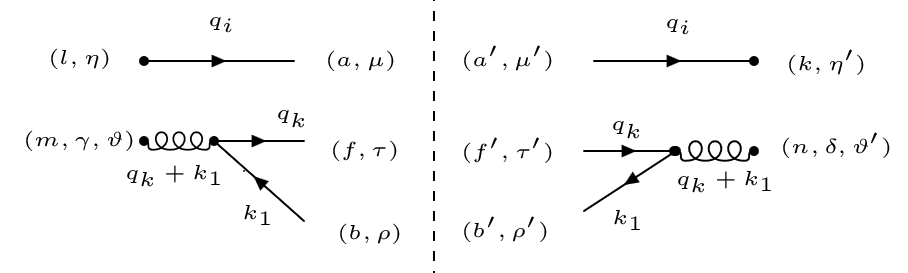
\includegraphics[scale=0.7]{images/QG/M2Squer.png}
%\end{figure}
%
%\begin{equation}
%\begin{split}
%|M_2|^2=\frac{{g_s}^2 {[T^m]_f}^b {[T^n]_{f}}^{b}}{4(k_1 \cdot q_k)(k_1\cdot q_k)}[\not{q_k}{\gamma}^{\gamma}\not{k_1}\:\: {\gamma}^{{\delta}}][\not{q_i}]
%\end{split}
%\end{equation}
%
%\pagebreak
%
%\section{Interference term}
%\begin{figure}[ht!]
%\centering
%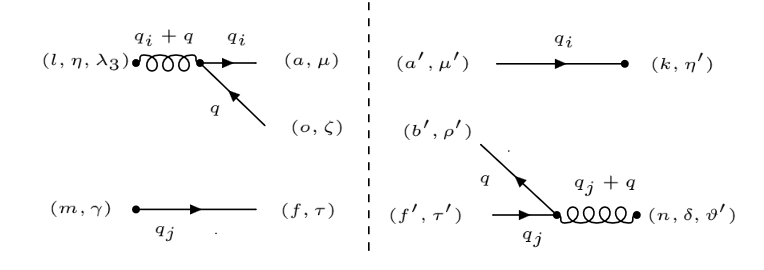
\includegraphics[scale=0.7]{images/QG/M1M2Dagger.png}
%\end{figure}
%
%
%\begin{equation}
%\begin{split}
%M_1\: {M_2}^{\dagger}=\frac{{g_s}^2 {[T^l]_a}^o {[T^n]_{f}}^{o}}{4(k_1 \cdot q_i)(k_1 \cdot q_k)}[\not{q_i}{\gamma}^{\eta}\not{k_1}][\: {\gamma}^{{\delta}}\not{q_k}]
%\end{split}
%\end{equation}
%
%\begin{equation}
%\begin{split}
%M_1\: {M_2}^{\dagger}=\frac{{g_s}^2 {[T^l]_a}^o {[T^n]_{f}}^{o}}{4(k_1\cdot q_i)(k_1 \cdot q_k)}[2\not{q_i}{k_1}^{\eta}-\not{q_i}\not{k_1}{\gamma}^{{\eta}}][\: g^{\delta \eta}{\gamma}_{{\eta}}\not{q_k}]
%\end{split}
%\end{equation}
%
%\begin{equation}
%\begin{split}
%M_1\: {M_2}^{\dagger}=\frac{{g_s}^2 {[T^l]_a}^o {[T^n]_{f}}^{o}}{4(k_1\cdot q_i)(k_1 \cdot q_k)}[2\not{q_i}\not{k_1}-d\not{q_i}\not{k_1}][\: g^{\delta \eta}][\not{q_k}]
%\end{split}
%\end{equation}
%
%\begin{equation}
%\begin{split}
%&M_1\: {M_2}^{\dagger}=(2-d)\frac{{g_s}^2 {[T^l]_a}^o {[T^n]_{f}}^{o}}{4y(1-\beta_1) (1-y)\:(p_i \cdot p_k)(p_i \cdot Q) }\\
%&[((\beta_1 -\alpha_1 y(\frac{Q^2}{2p_i \cdot Q}))\not{p_i} + y\alpha_1\not{Q} - \sqrt{y\alpha_1\beta_1}\not{n}_{\bot,1})\\&((\alpha_1 -y\beta_1(\frac{Q^2}{2p_i \cdot Q})) \not{p_i} + y\beta_1\not{Q} + \sqrt{y\alpha_1\beta_1}\not{n}_{\bot,1})][\: g^{\delta \eta}][\not{q_k}]
%\end{split}
%\end{equation}
%
%\begin{equation}
%\begin{split}
%&M_1\: {M_2}^{\dagger}=(2-d)\frac{{g_s}^2 {[T^l]_a}^o {[T^n]_{f}}^{o}}{4y(1-\beta_1) (1-y)\:(p_i \cdot p_k)(p_i \cdot Q) }\\
%&[\beta_1 \not{p_i}((\alpha_1 -y\beta_1(\frac{Q^2}{2p_i \cdot Q})) \not{p_i} + y\beta_1\not{Q}) ][\: g^{\delta \eta}][\not{q_k}]
%\end{split}
%\end{equation}
%
%\begin{equation}
%\begin{split}
%&M_1\: {M_2}^{\dagger}=(2-d)\frac{{g_s}^2 {[T^l]_a}^o {[T^n]_{f}}^{o}}{4y(1-\beta_1) (1-y)\:(p_i \cdot p_k)(p_i \cdot Q) }[y\beta_1^2 \not{p_i}\not{Q}) ][\: g^{\delta \eta}][\not{q_k}]
%\end{split}
%\end{equation}
%
%\section{$|M^{2}|$}
%
%\begin{equation}
%\begin{split}
%&|M|^{2}=|{M}_2|^{2}+|{M}_1|^{2}+2RE(M_1{M_2}^{\dagger})\\
%\end{split}
%\end{equation}  
\chapter{Gluon quark quark emission kernel}
\section{A daughter gluon from a parent quark}
\begin{figure}[ht!]
\centering
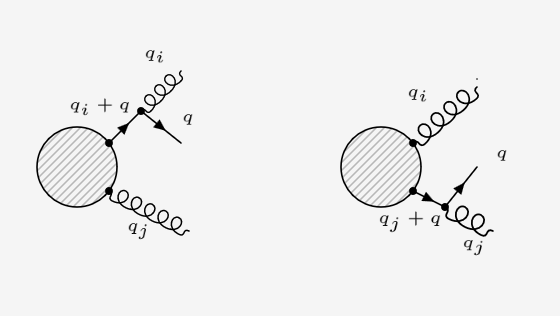
\includegraphics[width=0.85\textwidth]{images/GQ/GQDiagrams.png}
\end{figure}
Since the procedure here is the same as in the previous sections, only the final results are presented here.

\begin{figure}[ht!]
\centering
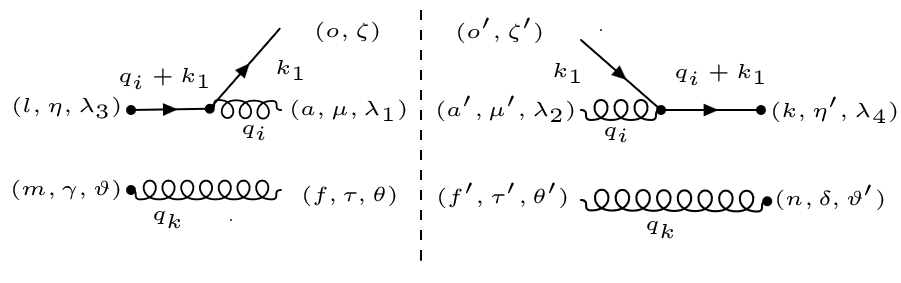
\includegraphics[scale=0.7]{images/GQ/M1Squer.png}
\end{figure}

%\begin{equation}
%\begin{split}
%|M_1|^2=-\frac{{g_s}^2 {[T^{a^{\prime}}]_k}^{o^{\prime}} {[T^a]_{o}}^{l}}{4(k_1 \cdot q_i)(k_1 \cdot q_i)}[(\not{q_i}+\not{k_1}) {\gamma}_{{\mu}}\not{k_1}\:{\gamma}^{\mu}(\not{q_i}+\not{k_1})\:][-{g^{\delta}}_{\gamma}]
%\end{split}
%\end{equation}
%
%\begin{equation}
%\begin{split}
%|M_1|^2=-(2-d)\frac{{g_s}^2 {[T^{a^{\prime}}]_k}^{o^{\prime}} {[T^a]_{o}}^{l}}{4(k_1 \cdot q_i)(k_1 \cdot q_i)}[(\not{q_i}+\not{k_1}) \not{k_1}(\not{q_i}+\not{k_1})\:][-{g^{\delta}}_{\gamma}]
%\end{split}
%\end{equation}
%
%\begin{equation}
%\begin{split}
%|M_1|^2=-(2-d)\frac{{g_s}^2 {[T^{a^{\prime}}]_k}^{o^{\prime}} {[T^a]_{o}}^{l}}{2(k_1 \cdot q_i)}[\not{q_i}][-{g^{\delta}}_{\gamma}]
%\end{split}
%\end{equation}
%
%\begin{equation}
%\begin{split}
%|M_1|^2=-(2-d)\frac{{g_s}^2 C_F}{2y\:p_i \cdot Q}
%[(\alpha_1 -y\beta_1(\frac{Q^2}{2p_i \cdot Q})) \not{p_i} + y\beta_1\not{Q} + \sqrt{y\alpha_1\beta_1}\not{n}_{\bot,1}][-{g^{\delta}}_{\gamma}]
%\end{split}
%\end{equation}

\begin{equation}
\begin{split}
|M_1|^2=(d-2)(1-\beta_1)\frac{{g_s}^2 C_F}{2y \:p_i \cdot Q}
[  \not{p_i}][-{g^{\delta}}_{\gamma}]
\end{split}
\end{equation}


\begin{figure}[ht!]
\centering
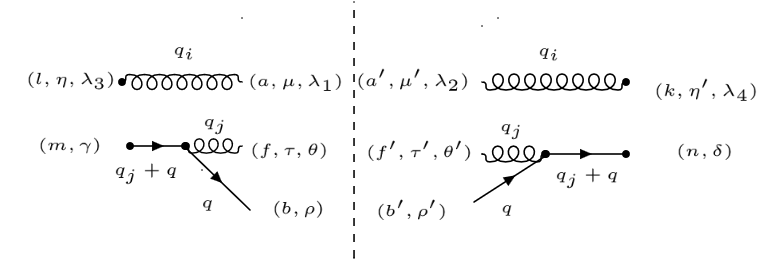
\includegraphics[scale=0.7]{images/GQ/M2Squer.png}
\end{figure}

\begin{equation}
\begin{split}
|M_2|^2=-\frac{{g_s}^2 C_F}{4(k_1 \cdot q_k)(k_1 \cdot q_k)}[(\not{q_k}+\not{k_1}) {\gamma}_{{\tau}^{\prime}}\not{k_1}{\gamma}^{\tau}(\not{q_k}+\not{k_1})][-g^{{\eta}{\eta}^{\prime}}]
\end{split}
\end{equation}

\begin{equation}
\begin{split}
|M_2|^2=(d-2)\frac{{g_s}^2 C_F}{4(k_1 \cdot q_k)}[\not{q_k}][-g^{{\eta}{\eta}^{\prime}}]
\end{split}
\end{equation}



%\begin{figure}[ht!]
%\centering
%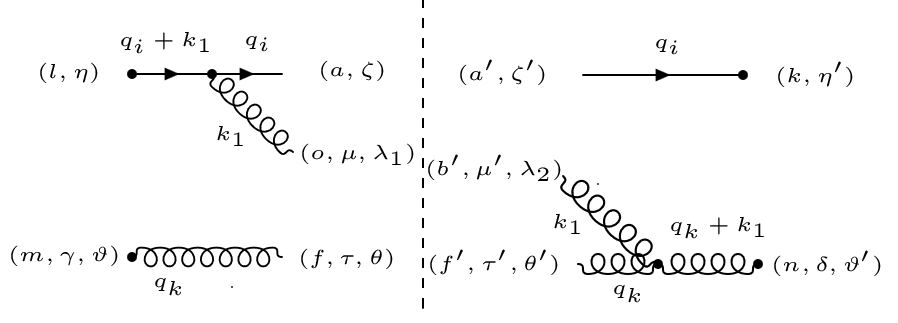
\includegraphics[scale=0.7]{images/GQ/M1M2DaggerGluon.png}
%\end{figure}

%\begin{equation}
%\begin{split}
%&M1{M_2}^{\dagger}=\frac{-{g_s}^2 {[T^{o}]_a}^{l} f^{\:f^{\prime}\: b^{\prime}\:n}}{4(k_1 \cdot q_i)(k_1 \cdot q_k)}[\not{q_i}{\gamma}_{\mu}(\not{k_1}+\not{q_i})\:]\\
%&[ (g^{{{\gamma}}{{\mu}}}(q_k-k_1)^{\delta}+g^{{{\mu}}{{\delta}}}(2k_1 +q_k)^{{\gamma}}-g^{\delta{{\gamma}}}(2q_k+k_1)^{{\mu}})]\\
%\end{split}
%\end{equation}
%
%\begin{equation}
%\begin{split}
%&M1{M_2}^{\dagger}=\frac{-{g_s}^2 {[T^{o}]_a}^{l} f^{\:f^{\prime}\: b^{\prime}\:n}}{4(k_1 \cdot q_i)(k_1 \cdot q_k)}[-\gamma_{\mu}\not{q_i}\not{k_1+2}(\not{k_1}+\not{q_i}){q_i}_{\mu}\:]\\
%&[ g^{{{\gamma}}{{\mu}}}(q_k-k_1)^{\delta}+g^{{{\mu}}{{\delta}}}(2k_1+q_k )^{{\gamma}}-g^{\delta{{\gamma}}}(2q_k+k_1)^{{\mu}}]\\
%\end{split}
%\end{equation}
%
%\begin{equation}
%\begin{split}
%&M1{M_2}^{\dagger}=\frac{-{g_s}^2 {[T^{o}]_a}^{l} f^{\:f^{\prime}\: b^{\prime}\:n}}{4 y(1-\beta_1) (1-y)\:(p_i \cdot p_k)(p_i \cdot Q)}\\
%&[-\gamma_{\mu}((\beta_1 -\alpha_1 y(\frac{Q^2}{2p_i \cdot Q}))\not{p_i} + y\alpha_1\not{Q})((\alpha_1 -y\beta_1(\frac{Q^2}{2p_i \cdot Q})) \not{p_i} + y\beta_1\not{Q})\\
%&+(2((\alpha_1 -y\beta_1(\frac{Q^2}{2p_i \cdot Q})) \not{p_i} + 2y\beta_1\not{Q}+2(\beta_1 -\alpha_1 y(\frac{Q^2}{2p_i \cdot Q}))\not{p_i} + 2y\alpha_1\not{Q})(\beta_1{q_i}_{\mu})\:]\\
%&[ g^{{{\gamma}}{{\mu}}}(-\alpha_1p_i)^{\delta}+g^{{{\mu}}{{\delta}}}(2\alpha_1p_i )^{{\gamma}}-g^{\delta{{\gamma}}}(\alpha_1p_i+(2-y)Q)^{{\mu}}]\\
%\end{split}
%\end{equation}
%
%\begin{equation}
%\begin{split}
%&M1{M_2}^{\dagger}=\frac{-{g_s}^2 C_F}{4 y(1-\beta_1) (1-y)\:(p_i \cdot p_k)(p_i \cdot Q)}\\
%&[-\gamma_{\mu}(y\beta_1^2)\not{p_i}\not{Q}+2(\not{p_i}+y\not{Q})(\beta_1{p_i}_{\mu})\:]\\
%&[ g^{{{\gamma}}{{\mu}}}(-\alpha_1p_i+\sqrt{1-y} p_k)^{\delta}+g^{{{\mu}}{{\delta}}}(2\alpha_1p_i+ \sqrt{1-y} p_k)^{{\gamma}}-g^{\delta{{\gamma}}}(\alpha_1p_i+2\sqrt{1-y} p_k)^{{\mu}}]\\
%\end{split}
%\end{equation}
%
%\begin{equation}
%\begin{split}
%&M1{M_2}^{\dagger}=\frac{-{g_s}^2 C_F}{4 y(1-\beta_1) (1-y)\:(p_i \cdot p_k)(p_i \cdot Q)}\\
%&[-\gamma_{\mu}(y\beta_1^2)\not{p_i}\not{Q}][ g^{{{\gamma}}{{\mu}}}(-\alpha_1p_i+\sqrt{1-y} p_k)^{\delta}+g^{{{\mu}}{{\delta}}}(2\alpha_1p_i+ \sqrt{1-y} p_k)^{{\gamma}}-g^{\delta{{\gamma}}}(\alpha_1p_i+2\sqrt{1-y} p_k)^{{\mu}}]\\
%&+[2(\not{p_i}+y\not{Q})(\beta_1{p_i}_{\mu})\:][ g^{{{\gamma}}{{\mu}}}(-\alpha_1p_i+\sqrt{1-y} p_k)^{\delta}+g^{{{\mu}}{{\delta}}}(2\alpha_1p_i+ \sqrt{1-y} p_k)^{{\gamma}}-g^{\delta{{\gamma}}}(\alpha_1p_i+2\sqrt{1-y} p_k)^{{\mu}}]\\
%\end{split}
%\end{equation}
%
%\begin{equation}
%\begin{split}
%&M1{M_2}^{\dagger}=\frac{-{g_s}^2 C_F}{4 y(1-\beta_1) (1-y)\:(p_i \cdot p_k)(p_i \cdot Q)}\\
%&[-\gamma_{\mu}(y\beta_1^2)\not{p_i}\not{Q}][ g^{{{\gamma}}{{\mu}}}(-\alpha_1p_i)^{\delta}+g^{{{\mu}}{{\delta}}}(\alpha_1p_i )^{{\gamma}}-g^{\delta{{\gamma}}}((2-y)Q)^{{\mu}}][{g^{\delta}}_{\gamma}]\\
%&+[2\beta_1(\not{p_i}+y\not{Q})\:][{p_i}^{\gamma} (-\alpha_1p_i)^{\delta}+{p_i}^{\delta}(2\alpha_1p_i )^{{\gamma}}-g^{\delta{{\gamma}}}(\alpha_1p_i+(2-y))Q\cdot p_i]\\
%\end{split}
%\end{equation}
%
%\begin{equation}
%\begin{split}
%&M1{M_2}^{\dagger}=\frac{-{g_s}^2 C_F}{4 y(1-\beta_1) (1-y)\:(p_i \cdot p_k)(p_i \cdot Q)}\\
%&[-\gamma_{\mu}(y\beta_1^2)\not{p_i}\not{Q}][-g^{\delta{{\gamma}}}(\alpha_1p_i+2\sqrt{1-y} p_k)^{{\mu}}]\\
%&+[2\beta_1(\not{p_i}+y\not{Q})\:][-g^{\delta{{\gamma}}}(\alpha_1p_i+2\sqrt{1-y})p_i\cdot p_k]\\
%\end{split}
%\end{equation}
%
%\begin{equation}
%\begin{split}
%&M1{M_2}^{\dagger}=\frac{-{g_s}^2 C_F}{4 y(1-\beta_1) (1-y)\:(p_i \cdot p_k)(p_i \cdot Q)}\\
%&[-2y\beta_1^2\sqrt{1-y} \not{p_k}\not{p_i}\not{Q}+4\sqrt{1-y}\beta_1(\not{p_i}+y\not{Q})p_i\cdot p_k][-g^{\delta{{\gamma}}}]\\
%\end{split}
%\end{equation}

%\begin{equation}
%\begin{split}
%&M1{M_2}^{\dagger}=\frac{-{g_s}^2 C_F}{y(1-\beta_1) (1-y)\:(p_i \cdot Q)}\sqrt{1-y}\beta_1[\not{p_i}][-g^{\delta{{\gamma}}}]\\
%\end{split}
%\end{equation}

\subsection{Interpretation of the result}

\begin{equation}
\begin{split}
&|M|^{2}=\frac{-{g_s}^2 C_F}{2y (1-y)\:(p_i \cdot Q)}[\not{p_i}][-g^{\delta{{\gamma}}}]\otimes [2RE(\frac{2\beta_1}{1-\beta_1})+(d-2)(1-\beta_1)]\\
\end{split}
\end{equation}

















       
\bibliographystyle{plain}
\bibliography{bibliography2}


%\listoftables
%\listoffigures
%\printindex

\appendix

First of all I would like to thank all those who supported me during the preparation of this work and who contributed a lot to the success of this work, in particular:\\
\\
PD Dr. Stefan Gieseke for his excellent care and patience.\\
\\
Prof. Dr. Dieter Zeppenfeld for the takeover of the second assessor.\\
\\
Dr. Simon Plätzer who gave me a helpful feedback and took the time to discuss this work.\\
My great thanks also go to Emma Simpson Dore, who proofread my work in numerous hours. She pointed out to me the weaknesses of my letter and showed me the right paths to reach my goal at work.\\
\\ 
Finally, I would like to thank my girlfriend Canan Kaman, who supported me in all things in this not always easy time.\\


 
         


 


\end{document}
